\documentclass[12pt,oneside]{book}

% Extra functionality for command parsing, colouring elements, and commentary
\usepackage{xparse}
\usepackage[table,dvipsnames]{xcolor}
\usepackage{comment}

% Make \today only show month and year
\usepackage[en-CA]{datetime2}
\DTMlangsetup[en-CA]{showdayofmonth=false}

% Manifest data
%------------------------------------------------------------------------------
% Your Information
%------------------------------------------------------------------------------

\newcommand{\thesisType}{Thesis}

\newcommand{\thesisTitle}{Adding Types and Theory Kinds to Drasil}
\newcommand{\thesisHalfTitle}{\thesisTitle}

\newcommand{\thesisAuthorName}{Jason Balaci}
\newcommand{\thesisAuthorNameShort}{J.\ Balaci}
\newcommand{\thesisAuthorCredentials}{B.Sc.}
\newcommand{\thesisSupervisor}{Dr.\ Jacques Carette}

\newcommand{\thesisTargetDegreeNameShort}{M.Sc.}
\newcommand{\thesisTargetDegreeName}{Master of Science}

\newcommand{\thesisTargetDegreeFocus}{Computer Science}
\newcommand{\thesisTargetDegree}{\thesisTargetDegreeName{} in \thesisTargetDegreeFocus{}}

\newcommand{\thesisInstitutionDepartmentShort}{Computing and Software}
\newcommand{\thesisInstitutionGraduateStudies}{School of Graduate Studies}
\newcommand{\thesisInstitutionDepartment}{Department of \thesisInstitutionDepartmentShort{}}
\newcommand{\thesisInstitution}{McMaster University}
\newcommand{\thesisCityProvince}{Hamilton, Ontario}

\newcommand{\thesisSubmissionYear}{\the\year{}}
\newcommand{\thesisSubmissionMonthYear}{\DTMtoday{}}

%------------------------------------------------------------------------------
% Metadata
%------------------------------------------------------------------------------

% The label placed on the last page of the front matter is used to find how many
% pages belong in the front matter (which are numbered with roman numerals
% instead of the traditional arabic numbering system). You only need to update
% this label value IF the "Declaration of Academic Achievement" is not the last
% page of your front matter.
\newcommand{\thesisLastPageOfFrontMatterLabel}{chap:declaration_of_academic_achievement}

%------------------------------------------------------------------------------
% Options
%------------------------------------------------------------------------------

% - COMPILE FOR PRINTING THE PDF                              (default = false)
%   If enabled, 'porthref'* links will appear in footnotes to assist readers.
\newif\ifcompilingforprinting
% \compilingforprintingtrue % Enable
\compilingforprintingfalse % Disable

% - DOUBLE SPACING                                            (default = 2x)
% \newcommand{\thesisSpacing}{\doublespacing}
% \newcommand{\thesisSpacing}{\singlespacing}
\newcommand{\thesisSpacing}{\linespread{1}}

% - QUESTION-DIRECTED WRITING & TO-DOS SWITCH                 (default = true)
%   If enabled, "writing directive" boxes will be displayed in the PDF
\newif\ifshowwritingdirectives
% \showwritingdirectivestrue % Show questions and to-do notes
\showwritingdirectivesfalse % Don't show questions and to-do notes

% - RESET FOOTNOTE NUMBERING FOR EACH PAGE                    (default = false)
%   If enabled, the footnote numbering will reset to 1 on each new page
\newif\ifresetfootnotecounter
% \resetfootnotecountertrue % Reset footnote numbering on each page
\resetfootnotecounterfalse % Don't reset footnote numbering on each page

% - MARGIN SIZES
\newcommand{\thesisMarginTop}{3.8cm}                        % ("official" = 3.8cm)
\newcommand{\thesisMarginBottom}{2.5cm}                     % ("official" = 2.5cm)
\newcommand{\thesisMarginInner}{2.5cm}                      % ("official" = 3.8cm)
\newcommand{\thesisMarginOuter}{2.5cm}                      % ("official" = 2.5cm)
\newcommand{\thesisMarginHeadheight}{15pt}                  % (default = 15pt)
\newcommand{\thesisTODOMarginSize}{2.25cm}                  % (default = 3.5cm)


% Configure font and file encodings, and language as Canadian English
\usepackage[T1]{fontenc}
\usepackage[utf8]{inputenc}
\usepackage[canadian]{babel}
\usepackage{lmodern}
\usepackage{anyfontsize}

% Math-related, but also generally helpful
\usepackage{proof}
\usepackage{amsmath}
\usepackage{amsfonts}
\usepackage{amsthm}
\usepackage{amssymb}
\usepackage{mathrsfs}
\usepackage{graphicx}
\usepackage{longtable}
\usepackage{svg}
\usepackage{mathpartir}
\usepackage{braket}

% Since LaTeX doesn't, and many fonts rarely, fully support unicode, we need to
% manually create characters to replace missing glyphs.
\usepackage{newunicodechar}
% At times, if you use raw unicode characters, you'll come across the following error:
% Missing character: There is no • (U+2022) in font ec-lmtt12!

% More, generally,
% Missing character: There is no `X` (U+`Y`) in font `Z`!

% To solve this  issue, we may manually replace instances of them with re-built
% copies of them. They may look a bit out of place because they don't follow the
% same font, but you can make them look decent if you replace them with simpler
% variants within the font. Try your best!

% For example, to resolve the above issue, we may use:
% \newunicodechar{•}{\(\cdot{}\)}

\newunicodechar{•}{\(\cdot{}\)}
\newunicodechar{‘}{\textquoteleft{}}
\newunicodechar{’}{\textquoteright{}}
\newunicodechar{≠}{\(\neq\)}


% Tiny package for easily grabbing the page count of the "main matter"
\usepackage{lastpage}

% For quotes, I wanted to put the "left bar" style. For implementation, Gonzalo
% Medina was very kind to create an example. It is based on:
% https://tex.stackexchange.com/a/50623
\usepackage{framed}
\usepackage[framemethod=TikZ]{mdframed}
\newmdenv[topline=false, rightline=false, bottomline=false,%
  linewidth=2pt, innerrightmargin=0pt, leftmargin=0pt,%
  innerleftmargin=5pt, skipabove=8pt, skipbelow=8pt]{mdleftbar}

\newmdenv[linewidth=2pt, linecolor=green, backgroundcolor=green!8, roundcorner=10pt,
  skipabove=8pt, skipbelow=8pt]{mdwritingdirectives}

% For nice captions and floating environments, such as for my code snippets
\usepackage{caption}
\usepackage{float}

% For inline-able list environments
\usepackage{paralist}

% Extra features for changing page widths ("adjustwidth" is a helpful environment!)
\usepackage{changepage}

% For code highlighting
\usepackage[newfloat,outputdir=build]{minted}
% Credits to Arash Esbati (https://tex.stackexchange.com/a/254177) for the
% listings-related component of minted usage.

\usemintedstyle{colorful}

% Configure page shape
\usepackage[
  a4paper,
  top=\thesisMarginTop{},
  bottom=\thesisMarginBottom{},
  inner=\thesisMarginInner{},
  outer=\thesisMarginOuter{},
  headheight=\thesisMarginHeadheight{},
]{geometry}

\usepackage{afterpage}

% Allow labelling enum items: Credits to: https://texblog.org/2012/03/21/cross-referencing-list-items/
\usepackage{enumitem}
\makeatletter
\def\namedlabel#1#2{\begingroup
    \textbf{#2}%
    \def\@currentlabel{#2}%
    \phantomsection\label{#1}\endgroup
}
\makeatother

\ifresetfootnotecounter
  % Make footnote counter reset for each new page.
  \usepackage{footnpag}
\fi

% Set spacing according to manifest
\usepackage{setspace}
\thesisSpacing{}

% Required for biblatex, but also adds functionality for quotation
\usepackage{csquotes}

% Credit to Gabriel Devenyi for this bibliography cfg:
% github.com/gdevenyi/mcmaster.latex
\usepackage[
  style=numeric-comp,
  backend=biber,
  sorting=none,
  backref=true,
  maxnames=99,
  alldates=iso,
  seconds=true
]{biblatex} % bibliography
\addbibresource{references.bib}

% Fancy Headers
\usepackage{fancyhdr}

% Allow more line breaks in URLs
\usepackage{xurl}

% Enable links within the document
\usepackage{hyperref}
\hypersetup{
  colorlinks=true,
  linkcolor=red,
  urlcolor=red,
  breaklinks=true,
  pdftitle={\thesisTitle{}},
  pdfauthor={\thesisAuthorName{}}
}
\urlstyle{rm} % Make URL styled fonts match hyperref's hrefs
\usepackage[nameinlink]{cleveref} % Fixes capitalization of internal references

% For abbreviations, we use "acro" package, and mfirstuc to help capitalize long
% versions normally
\usepackage{array}
\usepackage{mfirstuc}
\MFUhyphentrue % tell mfirstuc to capitalize hyphenated words

% Acronyms
\usepackage{acro}
% For one-offs,
% \DeclareAcronym{acronym}{short=short-version,long=long-version}

\newcommand{\newacr}[2]{\DeclareAcronym{#1}{short=\uppercase{#1},long=#2}}
\newcommand{\newacrs}[3]{\DeclareAcronym{#1}{short=#2,long=#3}}

% Alphabetically sorted list of acronyms
\newacr{adt}{Algebraic DataType}
\newacr{aml}{Algebraic Modelling Language}
\newacr{api}{Application Programming Interface}
\newacr{ast}{Algebraic Syntax Tree}
\newacr{cms}{Content Management System}
\newacr{cpu}{Central Processing Unit}
\newacr{csv}{Comma-Separated Values}
\newacr{dd}{Data Definition}
\newacr{dsl}{Domain-Specific Language}
\newacr{ffi}{Foreign Function Interface}
\newacr{gadt}{Generalized Algebraic DataType}
\newacr{gd}{General Definition}
\newacr{ghc}{Glasgow Haskell Compiler}
\newacr{gool}{Generic Object-oriented Language}
\newacr{gui}{Graphical User Interface}
\newacr{html}{HyperText Markup Language}
\newacr{ide}{Integrated Development Environment}
\newacr{im}{Instance Model}
\newacr{json}{JavaScript Object Notation}
\newacr{jvm}{Java Virtual Machine}
\newacr{kms}{Knowledge Management System}
\newacr{lss}{Literate Scientific Software}
\newacr{nasa}{National Aeronautics and Space Administration}
\newacr{ode}{Ordinary Differential Equation}
\newacr{oo}{Object-Oriented}
\newacr{pcm}{Phase Change Material}
\newacr{pd}{Proportional Derivative}
\newacr{pdf}{Portable Document Format}
\newacr{poc}{Proof Of Concept}
\newacr{rdbms}{Relational Database Management Systems}
\newacr{scs}{Scientific Computing Software}
\newacr{sis}{Software Interface Specification}
\newacr{sql}{Structured Query Language}
\newacr{srs}{Software Requirements Specification}
\newacr{stem}{science\, Technology\, Engineering\, and Mathematics}
\newacr{tm}{Theory Model}
\newacr{ttf}{Typed Tagless Final}
\newacr{uid}{Unique Identifier}
\newacr{url}{Uniform Resource Locator}
\newacr{wysiwyg}{What You See Is What You Get}

% Case Studies 
%   (note: I'm grouping these together and forcing "newacrs" usage, even when
%    seemingly unneeded because, otherwise, they won't group together at the 
%    bottom of the complete "acronyms" list.)
\newacrs{glassbr}{GlassBR}{Glass Breaking}
\newacrs{projectile}{Projectile}{Projectile}
\newacrs{sglpendulum}{SglPendulum}{Single Pendulum}
\newacrs{dblpendulum}{DblPendulum}{Double Pendulum}
\newacrs{gamephysics}{GamePhysics}{Game Physics}
\newacrs{hghc}{HGHC}{Heat Transfer Coefficients between Fuel and Cladding in Fuel Rods}
\newacrs{pdcontroller}{PDController}{Proportional Derivative controller}
\newacrs{swhs}{SWHS}{Solar Water Heating System}
\newacrs{nopcm}{NoPCM}{Solar Water Heating System Without PCM}
\newacrs{ssp}{SSP}{Slope Stability analysis Program}


%------------------------------------------------------------------------------
%- Extra commands for more functionality -- in particular, capitalizing the
%- long form of acronyms.
%------------------------------------------------------------------------------

% Defining \ACL - to capitalize all words in an acronym
% Credits to: https://tex.stackexchange.com/a/257896
\NewDocumentCommand\ACF{sm}{%
  \begingroup
    \acsetup{uppercase/cmd=\ecapitalisewords}%
    \IfBooleanTF{#1}{\Acf*{#2}}{\Acf{#2}}%
  \endgroup
}

\NewDocumentCommand\ACFP{sm}{%
  \begingroup
    \acsetup{uppercase/cmd=\ecapitalisewords}%
    \IfBooleanTF{#1}{\Acfp*{#2}}{\Acfp{#2}}%
  \endgroup
}

\NewDocumentCommand\ACL{sm}{%
  \begingroup
    \acsetup{uppercase/cmd=\ecapitalisewords}%
    \IfBooleanTF{#1}{\Acl*{#2}}{\Acl{#2}}%
  \endgroup
}

\NewDocumentCommand\ACLP{sm}{%
  \begingroup
    \acsetup{uppercase/cmd=\ecapitalisewords}%
    \IfBooleanTF{#1}{\Aclp*{#2}}{\Aclp{#2}}%
  \endgroup
}


% General Utility Functions
%%%%%%%%%%%%%%%%%%%%%%%%%%%%%%%%%%%%%%%%%%%%%%%%%%%%%%%%%%%%%%%%%%%%%%%%%%%%%%%
% QUESTION DIRECTED WRITING
\ifshowwritingdirectives
  \newenvironment{writingdirectives}{\begin{mdwritingdirectives}\centering\textbf{Writing Directives}\begin{itemize}}{\end{itemize}\end{mdwritingdirectives}}
\else
  \excludecomment{writingdirectives}
\fi

\newcommand{\wqanswer}[1]{\textit{#1}}

%%%%%%%%%%%%%%%%%%%%%%%%%%%%%%%%%%%%%%%%%%%%%%%%%%%%%%%%%%%%%%%%%%%%%%%%%%%%%%%
% SPACING OPTIONS
\newcommand{\thesisForceSingleSpacing}{\singlespacing}
\newcommand{\thesisForceDoubleSpacing}{\doublespacing}

%%%%%%%%%%%%%%%%%%%%%%%%%%%%%%%%%%%%%%%%%%%%%%%%%%%%%%%%%%%%%%%%%%%%%%%%%%%%%%%
% CASE STUDIES
\newcommand{\caseStudy}[1]{\ACL{#1} (\textit{\acs{#1}})}

%%%%%%%%%%%%%%%%%%%%%%%%%%%%%%%%%%%%%%%%%%%%%%%%%%%%%%%%%%%%%%%%%%%%%%%%%%%%%%%
% JUDGMENTS

\newcommand{\newrule}[2]{\begin{equation} \infer{#2}{#1} \end{equation}} % Adds to automatically numbered equations
\newcommand{\newlblrule}[3]{\begin{equation} \infer{#2}{#1} \label{#3}\end{equation}} % Adds to automatically numbered equations, with a label
\newcommand{\exampleRule}[2]{\[ \infer{#2}{#1} \]} % Does not add a number to equations

\newcommand{\Tau}{\mathrm{T}}
\newcommand{\ty}[1]{\texttt{#1} : \tau}

\newcommand{\ofTy}[2]{#1 : \texttt{#2}}

\newcommand{\numericTy}[1]{\ofTy{#1}{\texttt{Numerics($\Tau$)}}}
\newcommand{\negNumericTy}[1]{\ofTy{#1}{\texttt{NumericsWithNegation($\Tau$)}}}

%%%%%%%%%%%%%%%%%%%%%%%%%%%%%%%%%%%%%%%%%%%%%%%%%%%%%%%%%%%%%%%%%%%%%%%%%%%%%%%
% MATH

\newcommand{\bb}[1]{\mathbb{#1}}

%%%%%%%%%%%%%%%%%%%%%%%%%%%%%%%%%%%%%%%%%%%%%%%%%%%%%%%%%%%%%%%%%%%%%%%%%%%%%%%
% SYNTAX CHARTS
\newcommand{\startSyntaxTable}{\begin{longtable}{ r c c l c l }}
\newcommand{\newsyntaxRow}[5]{#1 & \( #2 \) & $::=$ & \texttt{#3} & $#4$ & #5 \\}
\newcommand{\syntaxRow}[3]{& & $\vert$ & \texttt{#1} & $#2$ & #3 \\}
\newcommand{\closeSyntaxTable}{\end{longtable}}

%%%%%%%%%%%%%%%%%%%%%%%%%%%%%%%%%%%%%%%%%%%%%%%%%%%%%%%%%%%%%%%%%%%%%%%%%%%%%%%
% Footnotes that only show "when compiling for printing"

\ifcompilingforprinting
  \newcommand{\printOnlyFootnote}[1]{\footnote{#1}}
  \newcommand{\printOnlyFootnoteText}[1]{\footnotetext{#1}}
  \newcommand{\printOnlyFootnoteMark}{\footnotemark}
\else
  \newcommand{\printOnlyFootnote}[1]{}
  \newcommand{\printOnlyFootnoteText}[1]{}
  \newcommand{\printOnlyFootnoteMark}{}
\fi

%%%%%%%%%%%%%%%%%%%%%%%%%%%%%%%%%%%%%%%%%%%%%%%%%%%%%%%%%%%%%%%%%%%%%%%%%%%%%%%
% Portable HREFs

% Common variant
\newcommand{\porthref}[2]{\href{#2}{#1}\printOnlyFootnote{\url{#2}}}
% Custom URLs
\newcommand{\porthreft}[3]{\href{#3}{#1}\printOnlyFootnote{\href{#3}{#2}}}
% Inside of some environments, footnote marks aren't registered properly, so we
% need to manually write the "text" part
\newcommand{\porthreftm}[2]{\href{#2}{#1\printOnlyFootnoteMark}}

%%%%%%%%%%%%%%%%%%%%%%%%%%%%%%%%%%%%%%%%%%%%%%%%%%%%%%%%%%%%%%%%%%%%%%%%%%%%%%%
% TODOs

% Generic Inlined TODOs
\newcommand{\intodo}[1]{\todo[inline]{#1}}

% Unimportant TODOs for "later" (i.e., finishing touches or changes immediately before submission)
\newcommand{\latertodo}[1]{\todo[backgroundcolor=Cyan]{\textit{Later}: #1}}

% "Important" TODOs
\newcommand{\imptodo}[1]{\todo[inline,backgroundcolor=Red]{\textbf{Important}: #1}}

% "Easy" TODOs
\newcommand{\easytodo}[1]{\todo[inline,backgroundcolor=SeaGreen]{\textit{Easy}: #1}}
\newcommand{\eztodo}[1]{\easytodo{#1}}

% "Tedious" TODOs
\newcommand{\tedioustodo}[1]{\todo[inline,backgroundcolor=PineGreen]{\textit{Needs time}: #1}}

% "Question" TODO Notes
\newcounter{todonoteQuestionsCtr}
\newcommand{\questiontodo}[1]{\stepcounter{todonoteQuestionsCtr}\todo[backgroundcolor=Lavender]{\textbf{Q \#\thetodonoteQuestionsCtr{}}: #1}}
\newcommand{\qtodo}[1]{\questiontodo{#1}}


%%%%%%%%%%%%%%%%%%%%%%%%%%%%%%%%%%%%%%%%%%%%%%%%%%%%%%%%%%%%%%%%%%%%%%%%%%%%%%%
% Haskell snippet
\newenvironment{code}{\captionsetup{type=listing,skip=14pt}}{}
\SetupFloatingEnvironment{listing}{name=Source Code, listname=List of Source Codes}
\crefname{listing}{source code}{source codes}
\Crefname{listing}{Source Code}{Source Codes}

\newenvironment{haskell}[3]
  {\VerbatimEnvironment\thesisForceSingleSpacing{}\begin{code}\captionof{listing}[#1]{\protect\porthreftm{#1}{#3}}\printOnlyFootnoteText{\protect\url{#3}}\label{lst:#2}\begin{minted}[frame=lines,framerule=2pt,breaklines]{haskell}}
  {\end{minted}\end{code}\thesisSpacing{}}

\newenvironment{codeSnippet}[4]
  {\VerbatimEnvironment\thesisForceSingleSpacing{}\begin{code}\captionof{listing}[#2]{\protect\porthreftm{#2}{#4}}\printOnlyFootnoteText{\protect\url{#4}}\label{lst:#3}\begin{minted}[frame=lines,framerule=2pt,breaklines]{#1}}
  {\end{minted}\end{code}\thesisSpacing{}}

\newenvironment{pseudohaskell}[2]
  {\VerbatimEnvironment\thesisForceSingleSpacing{}\begin{code}\captionof{listing}{Pseudocode: #1}\label{lst:#2}\begin{minted}[frame=lines,framerule=2pt,breaklines]{haskell}}
  {\end{minted}\end{code}\thesisSpacing{}}

\newenvironment{pseudocode}[3]
  {\VerbatimEnvironment\thesisForceSingleSpacing{}\begin{code}\captionof{listing}{Pseudocode: #2}\label{lst:#3}\begin{minted}[frame=lines,framerule=2pt,breaklines]{#1}}
  {\end{minted}\end{code}\thesisSpacing{}}

\newcommand{\inlineHs}[1]{\mintinline{haskell}|#1|}
\newcommand{\inlineCode}[2]{\mintinline{#1}|#2|}


% General Assets
%------------------------------------------------------------------------------
% Folders
%------------------------------------------------------------------------------

\newcommand{\assets}{assets}
\newcommand{\figureAssets}{\assets/figures}
\newcommand{\imageAssets}{\assets/images}
\newcommand{\tableAssets}{\assets/tables}
\newcommand{\codeAssets}{\assets/code}
\newcommand{\currentCode}{\codeAssets/current}
\newcommand{\originalCode}{\codeAssets/original}
\newcommand{\protoCode}{\codeAssets/prototypes}
\newcommand{\pseudoCode}{\codeAssets/pseudo}

%------------------------------------------------------------------------------
% Code
%------------------------------------------------------------------------------

% Command based on: https://tex.stackexchange.com/questions/266811/define-a-new-command-with-parameters-inside-newcommand
\newcommand{\codeName}[1]{\expandafter\newcommand\csname #1\endcsname{\inlineHs{#1}}}

\codeName{Chunk}
\codeName{ChunkDB}
\codeName{CodeExpr}
\codeName{ConceptChunk}
\codeName{ConstraintKinds}
\codeName{ConstraintSet}
\codeName{DataDefinition}
\codeName{DEModel}
\codeName{DefiningExpr}
\codeName{DifferentialModel}
\codeName{EquationalConstraints}
\codeName{EquationalModel}
\codeName{EquationalRealm}
\codeName{ExistentialQuantification}
\codeName{Expr}
\codeName{Express}
\codeName{GenDefn}
\codeName{HasChunkRefs}
\codeName{HasUID}
\codeName{IdeaDict}
\codeName{InstanceModel}
\codeName{Literal}
\codeName{ModelExpr}
\codeName{ModelKind}
\codeName{ModelKinds}
\codeName{MultiDefn}
\codeName{NewDEModel}
\codeName{ODEInfo}
\codeName{OthModel}
\codeName{QDefinition}
\codeName{QuantityDict}
\codeName{Relation}
\codeName{RelationConcept}
\codeName{relToQD}
\codeName{Space}
\codeName{Stage}
\codeName{Symbol}
\codeName{TheoryKind}
\codeName{TheoryKinds}
\codeName{TheoryModel}
\codeName{Typeable}
\codeName{TypeRep}
\codeName{UID}
\codeName{UnitDefn}

% Used for showing what the blue-highlighted text is, in the reading notes section
\codeName{ExampleText}


% "Current"
%--------------------------------------

% land pos rc convert to qd 
\newcommand{\currentLandPosRCtoQD}{\begin{haskell}{Converting ``landPosRC'' into a ``QDefinition''}{landPosRCtoQD}{https://github.com/JacquesCarette/Drasil/blob/7e2475041503d2ff79e522e0695408b8d32b576e/code/drasil-example/projectile/lib/Drasil/Projectile/IMods.hs\#L82-L83}
landPosQD :: QDefinition
landPosQD = mkQuantDef landPos E.landPosExpr
\end{haskell}
}
\newcommand{\refCurrentLandPosRCtoQD}{\Cref{lst:landPosRCtoQD}}

% land pos im to qd
\newcommand{\currentLandPosIMQD}{\begin{haskell}{``landPosIM'' Using ``QDefinition''}{landPosIMQD}{https://github.com/JacquesCarette/Drasil/blob/7e2475041503d2ff79e522e0695408b8d32b576e/code/drasil-example/projectile/lib/Drasil/Projectile/IMods.hs\#L76-L89}
landPosIM :: InstanceModel
landPosIM = imNoRefs (equationalModelN (nounPhraseSP "calculation of landing position") landPosQD)
  [qwC launSpeed $ UpFrom (Exc, exactDbl 0),
   qwC launAngle $ Bounded (Exc, exactDbl 0) (Exc, half $ sy pi_)]
  (qw landPos) [UpFrom (Exc, exactDbl 0)]
  (Just landPosDeriv) "calOfLandingDist" [angleConstraintNote, gravitationalAccelConstNote, landPosConsNote]

landPosQD :: QDefinition
landPosQD = mkQuantDef landPos E.landPosExpr

landPosDeriv :: Derivation
landPosDeriv = mkDerivName (phrase landPos) (weave [landPosDerivSents, map eS landPosDerivEqns])

landPosDerivSents :: [Sentence]
landPosDerivSents = [landPosDerivSent1, landPosDerivSent2, landPosDerivSent3, landPosDerivSent4]
\end{haskell}
}
\newcommand{\refCurrentLandPosIMQD}{\Cref{lst:landPosIMQD}}

% codeexpr
\newcommand{\currentCodeExprHaskell}{\begin{haskell}{CodeExpr Definition}{codeExprDefinition}{https://github.com/JacquesCarette/Drasil/blob/75db7d2bc8268e5d3600e8f36a960ced66fc4d60/code/drasil-code-base/lib/Language/Drasil/Code/Expr.hs\#L69-L137}
-- | Expression language where all terms also denote a term in GOOL
--   (i.e. translation is total and meaning preserving).
data CodeExpr where
  -- | Brings literals into the expression language.
  Lit      :: Literal -> CodeExpr


  -- | Takes an associative arithmetic operator with a list of expressions.
  AssocA   :: AssocArithOper -> [CodeExpr] -> CodeExpr
  -- | Takes an associative boolean operator with a list of expressions.
  AssocB   :: AssocBoolOper  -> [CodeExpr] -> CodeExpr
  -- | C stands for "Chunk", for referring to a chunk in an expression.
  --   Implicitly assumes that the chunk has a symbol.
  C        :: UID -> CodeExpr
  -- | A function call accepts a list of parameters and a list of named parameters.
  --   For example
  --
  --   * F(x) is (FCall F [x] []).
  --   * F(x,y) would be (FCall F [x,y]).
  --   * F(x,n=y) would be (FCall F [x] [(n,y)]).
  FCall    :: UID -> [CodeExpr] -> [(UID, CodeExpr)] -> CodeExpr
  -- | Actor creation given 'UID', parameters, and named parameters.
  New      :: UID -> [CodeExpr] -> [(UID, CodeExpr)] -> CodeExpr
  -- | Message an actor:
  --
  --   * 1st 'UID' is the actor,
  --   * 2nd 'UID' is the method.
  Message  :: UID -> UID -> [CodeExpr] -> [(UID, CodeExpr)] -> CodeExpr
  -- | Access a field of an actor:
  --
  --   * 1st 'UID' is the actor,
  --   * 2nd 'UID' is the field.
  Field    :: UID -> UID -> CodeExpr
  -- | For multi-case expressions, each pair represents one case.
  Case     :: Completeness -> [(CodeExpr, CodeExpr)] -> CodeExpr
  -- | Represents a matrix of expressions.
  Matrix   :: [[CodeExpr]] -> CodeExpr
  
  -- | Unary operation for most functions (eg. sin, cos, log, etc.).
  UnaryOp       :: UFunc -> CodeExpr -> CodeExpr
  -- | Unary operation for @Bool -> Bool@ operations.
  UnaryOpB      :: UFuncB -> CodeExpr -> CodeExpr
  -- | Unary operation for @Vector -> Vector@ operations.
  UnaryOpVV     :: UFuncVV -> CodeExpr -> CodeExpr
  -- | Unary operation for @Vector -> Number@ operations.
  UnaryOpVN     :: UFuncVN -> CodeExpr -> CodeExpr


  -- | Binary operator for arithmetic between expressions (fractional, power, and subtraction).
  ArithBinaryOp :: ArithBinOp -> CodeExpr -> CodeExpr -> CodeExpr
  -- | Binary operator for boolean operators (implies, iff).
  BoolBinaryOp  :: BoolBinOp -> CodeExpr -> CodeExpr -> CodeExpr
  -- | Binary operator for equality between expressions.
  EqBinaryOp    :: EqBinOp -> CodeExpr -> CodeExpr -> CodeExpr
  -- | Binary operator for indexing two expressions.
  LABinaryOp    :: LABinOp -> CodeExpr -> CodeExpr -> CodeExpr
  -- | Binary operator for ordering expressions (less than, greater than, etc.).
  OrdBinaryOp   :: OrdBinOp -> CodeExpr -> CodeExpr -> CodeExpr
  -- | Binary operator for @Vector x Vector -> Vector@ operations (cross product).
  VVVBinaryOp   :: VVVBinOp -> CodeExpr -> CodeExpr -> CodeExpr
  -- | Binary operator for @Vector x Vector -> Number@ operations (dot product).
  VVNBinaryOp   :: VVNBinOp -> CodeExpr -> CodeExpr -> CodeExpr


  -- | Operators are generalized arithmetic operators over a 'DomainDesc'
  --   of an 'Expr'.  Could be called BigOp.
  --   ex: Summation is represented via 'Add' over a discrete domain.
  Operator :: AssocArithOper -> DiscreteDomainDesc CodeExpr CodeExpr -> CodeExpr -> CodeExpr
  -- | The expression is an element of a space.
  -- IsIn     :: Expr -> Space -> Expr
  -- | A different kind of 'IsIn'. A 'UID' is an element of an interval.
  RealI    :: UID -> RealInterval CodeExpr CodeExpr -> CodeExpr
\end{haskell}
}
\newcommand{\refCurrentCodeExprHaskell}{\Cref{lst:codeExprDefinition}}

% codeexpr ttf
\newcommand{\currentCodeExprTTFHaskell}{\begin{haskell}{CodeExpr TTF Encoding}{codeExprDefinitionTTF}{https://github.com/JacquesCarette/Drasil/blob/75db7d2bc8268e5d3600e8f36a960ced66fc4d60/code/drasil-code-base/lib/Language/Drasil/Code/Expr/Class.hs\#L10-L28}
class CodeExprC r where
  -- | Constructs a CodeExpr for actor creation (constructor call)
  new :: (Callable f, HasUID f, CodeIdea f) => f -> [r] -> r
  
  -- | Constructs a CodeExpr for actor creation (constructor call) that uses named arguments
  newWithNamedArgs :: (Callable f, HasUID f, CodeIdea f, HasUID a, 
    IsArgumentName a) => f -> [r] -> [(a, r)] -> r
  
  -- | Constructs a CodeExpr for actor messaging (method call)
  message :: (Callable f, HasUID f, CodeIdea f, HasUID c, HasSpace c, CodeIdea c) 
    => c -> f -> [r] -> r
  
  -- | Constructs a CodeExpr for actor messaging (method call) that uses named arguments
  msgWithNamedArgs :: (Callable f, HasUID f, CodeIdea f, HasUID c, HasSpace c, 
    CodeIdea c, HasUID a, IsArgumentName a) => c -> f -> [r] -> [(a, r)] -> 
    r
  
  -- | Constructs a CodeExpr representing the field of an actor
  field :: CodeVarChunk -> CodeVarChunk -> r
\end{haskell}
}
\newcommand{\refCurrentCodeExprTTFHaskell}{\Cref{lst:codeExprDefinitionTTF}}

% constraintset
\newcommand{\currentConstraintSetHaskell}{\begin{haskell}{ConstraintSet Definition}{curConstraintSet}{https://github.com/JacquesCarette/Drasil/blob/9f435cbb9bcda515d765c551606d1f4e3d9fc101/code/drasil-theory/lib/Theory/Drasil/ConstraintSet.hs\#L15-L19}
-- | 'ConstraintSet's are sets of invariants that always hold for underlying domains.
data ConstraintSet e = CL {
    _con  :: ConceptChunk,
    _invs :: NE.NonEmpty e
}
\end{haskell}
}
\newcommand{\refCurrentConstraintSetHaskell}{\Cref{lst:curConstraintSet}}

% definingexpr
\newcommand{\currentDefiningExprHaskell}{\begin{haskell}{Definition Possibility}{curDefiningExpr}{https://github.com/JacquesCarette/Drasil/blob/dc3674274edb00b1ae0d63e04ba03729e1dbc6f9/code/drasil-theory/lib/Theory/Drasil/MultiDefn.hs\#L19-L27}
-- | 'DefiningExpr' are the data that make up a (quantity) definition, namely
--   the description, the defining (rhs) expression and the context domain(s).
--   These are meant to be 'alternate' but equivalent definitions for a single concept.
data DefiningExpr e = DefiningExpr {
  _deUid  :: UID,      -- ^ UID
  _cd     :: [UID],    -- ^ Concept domain
  _rvDesc :: Sentence, -- ^ Defining description/statement
  _expr   :: e         -- ^ Defining expression
}
\end{haskell}
}
\newcommand{\refCurrentDefiningExprHaskell}{\Cref{lst:curDefiningExpr}}

% example of gathering chunks into lists
\newcommand{\currentExampleGatherChunkIntoListsHaskell}{\begin{haskell}{Example of Current Chunk Gathering Into A List}{curExampleGatherChunkIntoLists}{https://github.com/JacquesCarette/Drasil/blob/dc3674274edb00b1ae0d63e04ba03729e1dbc6f9/code/drasil-example/glassbr/lib/Drasil/GlassBR/DataDefs.hs\#L36-L39}
dataDefs :: [DataDefinition]
dataDefs = [risk, hFromt, loadDF, strDisFac, nonFL, glaTyFac,
  dimLL, tolPre, tolStrDisFac, standOffDis, aspRat, eqTNTWDD, probOfBreak,
  calofCapacity, calofDemand]
\end{haskell}
}
\newcommand{\refCurrentExampleGatherChunkIntoListsHaskell}{\Cref{lst:curExampleGatherChunkIntoLists}}

% example of gathering chunk lists into chunkdb
\newcommand{\currentExampleGatherChunkListsIntoDBHaskell}{\begin{haskell}{Example of Current Gathering Chunk Lists Into the Database}{curExampleGatherChunkListsIntoDB}{https://github.com/JacquesCarette/Drasil/blob/dc3674274edb00b1ae0d63e04ba03729e1dbc6f9/code/drasil-example/glassbr/lib/Drasil/GlassBR/Body.hs\#L128-L137}
symbMap :: ChunkDB
symbMap = cdb thisSymbols (map nw acronyms ++ map nw thisSymbols ++ map nw con
  ++ map nw con' ++ map nw terms ++ map nw doccon ++ map nw doccon' ++ map nw educon
  ++ [nw sciCompS] ++ map nw compcon ++ map nw mathcon ++ map nw mathcon'
  ++ map nw softwarecon ++ map nw terms ++ [nw lateralLoad, nw materialProprty]
   ++ [nw distance, nw algorithm] ++
  map nw fundamentals ++ map nw derived ++ map nw physicalcon)
  (map cw symb ++ terms ++ Doc.srsDomains) (map unitWrapper [metre, second, kilogram]
  ++ map unitWrapper [pascal, newton]) GB.dataDefs iMods [] tMods concIns section
  labCon []
\end{haskell}
}
\newcommand{\refCurrentExampleGatherChunkListsIntoDBHaskell}{\Cref{lst:curExampleGatherChunkListsIntoDB}}

% example equational constraints
\newcommand{\currentExampleEquationalConstraintsHaskell}{\begin{figure}
    \centering
    \caption{\porthreftm{Constraints on a System}{https://github.com/JacquesCarette/Drasil/blob/54347382ee4eac6c38b52a93d4018709ee3ab948/examples/ssp/SRS/srs/SSP_SRS.html}}
    \label{fig:exampleEquationalConstraints}
    \printOnlyFootnoteText{Rendered from: \url{https://github.com/JacquesCarette/Drasil/blob/54347382ee4eac6c38b52a93d4018709ee3ab948/examples/ssp/SRS/srs/SSP_SRS.html}}

    \includegraphics[width=0.8\linewidth]{\figExampleEquationalConstraints}
\end{figure}
}
\newcommand{\refCurrentExampleEquationalConstraintsHaskell}{\Cref{lst:exampleEquationalConstraints}}

% example equational realm
\newcommand{\currentExampleEquationalRealmHaskell}{\begin{haskell}{Example of Equational Realm: Horizontal Force}{exampleEquationalRealm}{https://github.com/JacquesCarette/Drasil/blob/dc3674274edb00b1ae0d63e04ba03729e1dbc6f9/code/drasil-example/dblpendulum/lib/Drasil/DblPendulum/GenDefs.hs\#L212-L230}
-------------------------------------------------
-- Horizontal force acting on the first object --
-------------------------------------------------
xForceGD_1 :: GenDefn
xForceGD_1 = gdNoRefs (equationalRealmU "xForce1" xForceMD_1)
        (getUnit force) (Just xForceDeriv_1) "xForce1" []

xForceMD_1 :: MultiDefn ModelExpr
xForceMD_1 = mkMultiDefnForQuant quant EmptyS defns
    where quant = mkQuant' "force" (horizontalForce `onThe` firstObject)
                    Nothing Real (symbol force) (getUnit force)
          defns = NE.fromList [
                    mkDefiningExpr "xForceWithMass1"
                      [] EmptyS $ express $ forceGQD ^. defnExpr,
                    mkDefiningExpr "xForceWithAngle1"
                      [] EmptyS E.xForceWithAngle_1]

xForceDeriv_1 :: Derivation
xForceDeriv_1 = mkDerivName (phraseNP (force `onThe` firstObject)) [eS' xForceMD_1]
\end{haskell}
}
\newcommand{\refCurrentExampleEquationalRealmHaskell}{\Cref{lst:exampleEquationalRealm}}

% expr
\newcommand{\currentExprHaskell}{\begin{haskell}{Original Expression language}{origExpr}{https://github.com/JacquesCarette/Drasil/blob/9c26b43d3e30c3f618e534a3f176a5152729af74/code/drasil-lang/Language/Drasil/Expr.hs\#L40-L82}
-- | Drasil Expressions
data Expr where
  Dbl      :: Double -> Expr
  Int      :: Integer -> Expr
  Str      :: String -> Expr
  Perc     :: Integer -> Integer -> Expr
  AssocA   :: ArithOper -> [Expr] -> Expr
  AssocB   :: BoolOper  -> [Expr] -> Expr
  -- | Derivative, syntax is:
  --   Type (Partial or total) -> principal part of change -> with respect to
  --   For example: Deriv Part y x1 would be (dy/dx1)
  Deriv    :: DerivType -> Expr -> UID -> Expr
  -- | C stands for "Chunk", for referring to a chunk in an expression.
  --   Implicitly assumes has a symbol.
  C        :: UID -> Expr
  -- | F(x) is (FCall F [x] []) or similar.
  --   FCall accepts a list of params and a list of named params.
  --   F(x,y) would be (FCall F [x,y]) or sim.
  --   F(x,n=y) would be (FCall F [x] [(n,y)]).
  FCall    :: UID -> [Expr] -> [(UID, Expr)] -> Expr
  -- | Actor creation given UID and parameters 
  New      :: UID -> [Expr] -> [(UID, Expr)] -> Expr 
  -- | Message an actor: 
  --   1st UID is the actor, 
  --   2nd UID is the method
  Message  :: UID -> UID -> [Expr] -> [(UID, Expr)] -> Expr
  -- | Access a field of an actor:
  --   1st UID is the actor,
  --   2nd UID is the field
  Field :: UID -> UID -> Expr
  -- | For multi-case expressions, each pair represents one case
  Case     :: Completeness -> [(Expr,Relation)] -> Expr
  Matrix   :: [[Expr]] -> Expr
  UnaryOp  :: UFunc -> Expr -> Expr
  BinaryOp :: BinOp -> Expr -> Expr -> Expr
  -- | Operators are generalized arithmetic operators over a |DomainDesc|
  --   of an |Expr|.  Could be called |BigOp|.
  --   ex: Summation is represented via |Add| over a discrete domain
  Operator :: ArithOper -> DomainDesc Expr Expr -> Expr -> Expr
  -- | element of
  IsIn     :: Expr -> Space -> Expr 
  -- | a different kind of 'element of'
  RealI    :: UID -> RealInterval Expr Expr -> Expr 
\end{haskell}
}
\newcommand{\refCurrentExprHaskell}{\Cref{lst:curExpr}}

% expr bi-directional typing instance
\newcommand{\currentExprBidirTypeCheckingHaskell}{\begin{haskell}{Expr's Bi-directional Type Checking Instance}{curBidirTypechecking}{https://github.com/JacquesCarette/Drasil/blob/b6de97ddc3011f513f67abd6043df176c30ba1a3/code/drasil-lang/lib/Language/Drasil/Expr/Lang.hs\#L202-L385}
instance Typed Expr Space where
  check :: TypingContext Space -> Expr -> Space -> Either Space TypeError
  check = typeCheckByInfer

  infer :: TypingContext Space -> Expr -> Either Space TypeError
  infer cxt (Lit lit) = infer cxt lit

  infer cxt (AssocA op exs) = allOfType cxt exs sp sp
      $ "Associative arithmetic operation expects all operands to be of the same expected type (" ++ show sp ++ ")."
    where
      sp = assocArithOperToTy op

  infer cxt (AssocB _ exs) = allOfType cxt exs S.Boolean S.Boolean
    $ "Associative boolean operation expects all operands to be of the same type (" ++ show S.Boolean ++ ")."

  infer cxt (C uid) = inferFromContext cxt uid

  infer cxt (FCall uid exs) = case (inferFromContext cxt uid, map (infer cxt) exs) of
    (Left (S.Function params out), exst) -> if NE.toList params == lefts exst
      then Left out
      else Right $ "Function `" ++ show uid ++ "` expects parameters of types: " ++ show params ++ ", but received: " ++ show (lefts exst) ++ "."
    (Left s, _) -> Right $ "Function application on non-function `" ++ show uid ++ "` (" ++ show s ++ ")."
    (Right x, _) -> Right x

  infer cxt (Case _ ers)
    | null ers = Right "Case contains no expressions, no type to infer."
    | all (\(ne, _) -> infer cxt ne == eT) (tail ers) = eT
    | otherwise = Right "Expressions in case statement contain different types."
      where
        (fe, _) = head ers
        eT = infer cxt fe

  infer cxt (Matrix exss)
    | null exss = Right "Matrix has no rows."
    | null $ head exss = Right "Matrix has no columns."
    | allRowsHaveSameColumnsAndSpace = Left $ S.Matrix rows columns t
    | otherwise = Right "Not all rows have the same number of columns or the same value types."
    where
        rows = length exss
        columns = if rows > 0 then length $ head exss else 0
        sss = map (map (infer cxt)) exss
        expT = head $ head sss
        allRowsHaveSameColumnsAndSpace
          = either
              (\_ -> all (\ r -> length r == columns && all (== expT) r) sss)
              (const False) expT
        (Left t) = expT

  infer cxt (UnaryOp uf ex) = case infer cxt ex of
    Left sp -> case uf of
      Abs -> if S.isBasicNumSpace sp && sp /= S.Natural
        then Left sp
        else Right $ "Numeric 'absolute' value operator only applies to, non-natural, numeric types. Received `" ++ show sp ++ "`."
      Neg -> if S.isBasicNumSpace sp && sp /= S.Natural
        then Left sp
        else Right $ "Negation only applies to, non-natural, numeric types. Received `" ++ show sp ++ "`."
      Exp -> if sp == S.Real || sp == S.Integer then Left S.Real else Right $ show Exp ++ " only applies to reals."
      x -> if sp == S.Real
        then Left S.Real
        else Right $ show x ++ " only applies to Reals. Received `" ++ show sp ++ "`."
    x       -> x

  infer cxt (UnaryOpB Not ex) = case infer cxt ex of
    Left S.Boolean -> Left S.Boolean
    Left sp        -> Right $ "¬ on non-boolean operand, " ++ show sp ++ "."
    x              -> x

  infer cxt (UnaryOpVV NegV e) = case infer cxt e of
    Left (S.Vect sp) -> if S.isBasicNumSpace sp && sp /= S.Natural
      then Left $ S.Vect sp
      else Right $ "Vector negation only applies to, non-natural, numbered vectors. Received `" ++ show sp ++ "`."
    Left sp -> Right $ "Vector negation should only be applied to numeric vectors. Received `" ++ show sp ++ "`."
    x -> x

  infer cxt (UnaryOpVN Norm e) = case infer cxt e of
    Left (S.Vect S.Real) -> Left S.Real
    Left sp -> Right $ "Vector norm only applies to vectors of real numbers. Received `" ++ show sp ++ "`."
    x -> x

  infer cxt (UnaryOpVN Dim e) = case infer cxt e of
    Left (S.Vect _) -> Left S.Integer -- FIXME: I feel like Integer would be more usable, but S.Natural is the 'real' expectation here
    Left sp -> Right $ "Vector 'dim' only applies to vectors. Received `" ++ show sp ++ "`."
    x -> x

  infer cxt (ArithBinaryOp Frac l r) = case (infer cxt l, infer cxt r) of
    (Left lt, Left rt) -> if S.isBasicNumSpace lt && lt == rt
      then Left lt
      else Right $ "Fractions/divisions should only be applied to the same numeric typed operands. Received `" ++ show lt ++ "` / `" ++ show rt ++ "`."
    (_      , Right e) -> Right e
    (Right e, _      ) -> Right e

  infer cxt (ArithBinaryOp Pow l r) = case (infer cxt l, infer cxt r) of
    (Left lt, Left rt) -> if S.isBasicNumSpace lt && (lt == rt || (lt == S.Real && rt == S.Integer))
      then Left lt
      else Right $
        "Powers should only be applied to the same numeric type in both operands, or real base with integer exponent. Received `" ++ show lt ++ "` ^ `" ++ show rt ++ "`."
    (_      , Right x) -> Right x
    (Right x, _      ) -> Right x

  infer cxt (ArithBinaryOp Subt l r) = case (infer cxt l, infer cxt r) of
    (Left lt, Left rt) -> if S.isBasicNumSpace lt && lt == rt
      then Left lt
      else Right $ "Both operands of a subtraction must be the same numeric type. Received `" ++ show lt ++ "` - `" ++ show rt ++ "`."
    (_, Right re) -> Right re
    (Right le, _) -> Right le

  infer cxt (BoolBinaryOp _ l r) = case (infer cxt l, infer cxt r) of
    (Left S.Boolean, Left S.Boolean) -> Left S.Boolean
    (Left lt, Left rt) -> Right $ "Boolean expression contains non-boolean operand. Received `" ++ show lt ++ "` & `" ++ show rt ++ "`."
    (_     , Right er) -> Right er
    (Right el, _     ) -> Right el

  infer cxt (EqBinaryOp _ l r) = case (infer cxt l, infer cxt r) of
    (Left lt, Left rt) -> if lt == rt
      then Left S.Boolean
      else Right $ "Both operands of an (in)equality (=/≠) must be of the same type. Received `" ++ show lt ++ "` & `" ++ show rt ++ "`."
    (_, Right re) -> Right re
    (Right le, _) -> Right le

  infer cxt (LABinaryOp Index l n) = case (infer cxt l, infer cxt n) of
    (Left (S.Vect lt), Left nt) -> if nt == S.Integer || nt == S.Natural -- I guess we should only want it to be natural numbers, but integers or naturals is fine for now
      then Left lt
      else Right $ "List accessor not of type Integer nor Natural, but of type `" ++ show nt ++ "`"
    (Left lt         , Left _)  -> Right $ "List accessor expects a list/vector, but received `" ++ show lt ++ "`."
    (_               , Right e) -> Right e
    (Right e         , _      ) -> Right e

  infer cxt (OrdBinaryOp _ l r) = case (infer cxt l, infer cxt r) of
    (Left lt, Left rt) -> if S.isBasicNumSpace lt && lt == rt
      then Left S.Boolean
      else Right $ "Both operands of a numeric comparison must be the same numeric type, got: " ++ show lt ++ ", " ++ show rt ++ "."
    (_, Right re) -> Right re
    (Right le, _) -> Right le

  infer cxt (VVVBinaryOp Cross l r) = case (infer cxt l, infer cxt r) of
    (Left lTy, Left rTy) -> if lTy == rTy && S.isBasicNumSpace lTy && lTy /= S.Natural
      then Left lTy
      else Right $ "Vector cross product expects both operands to be vectors of non-natural numbers. Received `" ++ show lTy ++ "` X `" ++ show rTy ++ "`."
    (_       , Right re) -> Right re
    (Right le, _       ) -> Right le

  infer cxt (VVNBinaryOp Dot l r) = case (infer cxt l, infer cxt r) of
    (Left lt@(S.Vect lsp), Left rt@(S.Vect rsp)) -> if lsp == rsp && S.isBasicNumSpace lsp
      then Left lsp
      else Right $ "Vector dot product expects same numeric vector types, but found `" ++ show lt ++ "` · `" ++ show rt ++ "`."
    (Left lsp, Left rsp) -> Right $ "Vector dot product expects vector operands. Received `" ++ show lsp ++ "` · `" ++ show rsp ++ "`."
    (_, Right rx) -> Right rx
    (Right lx, _) -> Right lx

  infer cxt (Operator aao (S.BoundedDD _ _ bot top) body) = 
    let expTy = assocArithOperToTy aao in
    case (infer cxt bot, infer cxt top, infer cxt body) of
      (Left botTy, Left topTy, Left bodyTy) -> if botTy == S.Integer
        then if topTy == S.Integer
          then if expTy == bodyTy
            then Left expTy
            else Right $ "'Big' operator range body not Integer, found: " ++ show bodyTy ++ "."
          else Right $ "'Big' operator range top not Integer, found: " ++ show topTy ++ "."
        else Right $ "'Big' operator range bottom not of expected type: " ++ show expTy ++ ", found: " ++ show botTy ++ "."
      (_         , _         , Right x    ) -> Right x
      (_         , Right x   , _          ) -> Right x
      (Right x   , _         , _          ) -> Right x

  infer cxt (RealI uid ri) = 
    case (inferFromContext cxt uid, riTy ri) of
      (Left S.Real, Left riSp) -> if riSp == S.Real
        then Left S.Boolean
        else Right $
          "Real interval expects interval bounds to be of type Real, but received: " ++ show riSp ++ "."
      (Left uidSp, _         ) -> Right $
        "Real interval expects variable to be of type Real, but received `" ++ show uid ++ "` of type `" ++ show uidSp ++ "`."
      (_          , Right x  ) -> Right x
      (Right x    , _        ) -> Right x
    where
      riTy :: RealInterval Expr Expr -> Either Space TypeError
      riTy (S.Bounded (_, lx) (_, rx)) = case (infer cxt lx, infer cxt rx) of
        (Left lt, Left rt) -> if lt == rt
          then Left lt
          else Right $
            "Bounded real interval contains mismatched types for bottom and top. Received `" ++ show lt ++ "` to `" ++ show rt ++ "`."
        (_      , Right x) -> Right x
        (Right x, _      ) -> Right x
      riTy (S.UpTo (_, x)) = infer cxt x
      riTy (S.UpFrom (_, x)) = infer cxt x
\end{haskell}
}
\newcommand{\refCurrentExprBidirTypeCheckingHaskell}{\Cref{lst:curBidirTypechecking}}

% express
\newcommand{\currentExpressHaskell}{\begin{haskell}{Express Typeclass}{curExpress}{https://github.com/JacquesCarette/Drasil/blob/dc3674274edb00b1ae0d63e04ba03729e1dbc6f9/code/drasil-lang/lib/Language/Drasil/ExprClasses.hs\#L9-L11}
-- | Data that can be expressed using 'ModelExpr'.
class Express c where
  express :: c -> ModelExpr
\end{haskell}
}
\newcommand{\refCurrentExpressHaskell}{\Cref{lst:curExpress}}

% exprTTF
\newcommand{\currentExprTTFHaskell}{\begin{haskell}{Expr Constructor Encoding (TTF)}{curExprTTF}{https://github.com/JacquesCarette/Drasil/blob/f979892d095cceed4d062afb17bd9654bcda4fe2/code/drasil-lang/lib/Language/Drasil/Expr/Class.hs\#L86-L209}
class ExprC r where
  infixr 8 $^
  infixl 7 $/
  infixr 4 $=
  infixr 9 $&&
  infixr 9 $||
  
  lit :: Literal -> r

  -- * Binary Operators
  
  ($=), ($!=) :: r -> r -> r
  
  -- | Smart constructor for ordering two equations.
  ($<), ($>), ($<=), ($>=) :: r -> r -> r
  
  -- | Smart constructor for the dot product of two equations.
  ($.) :: r -> r -> r
  
  -- | Add two expressions (Integers).
  addI :: r -> r -> r
  
  -- | Add two expressions (Real numbers).
  addRe :: r -> r -> r
  
  -- | Multiply two expressions (Integers).
  mulI :: r -> r -> r
  
  -- | Multiply two expressions (Real numbers).
  mulRe :: r -> r -> r
  
  ($-), ($/), ($^) :: r -> r -> r
  
  ($=>), ($<=>) :: r -> r -> r
  
  ($&&), ($||) :: r -> r -> r
  
  -- | Smart constructor for taking the absolute value of an expression.
  abs_ :: r -> r
  
  -- | Smart constructor for negating an expression.
  neg :: r -> r 
  
  -- | Smart constructor to take the log of an expression.
  log :: r -> r
  
  -- | Smart constructor to take the ln of an expression.
  ln :: r -> r
  
  -- | Smart constructor to take the square root of an expression.
  sqrt :: r -> r
  
  -- | Smart constructor to apply sin to an expression.
  sin :: r -> r
  
  -- | Smart constructor to apply cos to an expression.
  cos :: r -> r 
  
  -- | Smart constructor to apply tan to an expression.
  tan :: r -> r
  
  -- | Smart constructor to apply sec to an expression.
  sec :: r -> r 
  
  -- | Smart constructor to apply csc to an expression.
  csc :: r -> r
  
  -- | Smart constructor to apply cot to an expression.
  cot :: r -> r 
  
  -- | Smart constructor to apply arcsin to an expression.
  arcsin :: r -> r 
  
  -- | Smart constructor to apply arccos to an expression.
  arccos :: r -> r 
  
  -- | Smart constructor to apply arctan to an expression.
  arctan :: r -> r 
  
  -- | Smart constructor for the exponential (base e) function.
  exp :: r -> r
  
  -- | Smart constructor for calculating the dimension of a vector.
  dim :: r -> r
  
  -- | Smart constructor for calculating the normal form of a vector.
  norm :: r -> r
  
  -- | Smart constructor for negating vectors.
  negVec :: r -> r
  
  -- | Smart constructor for applying logical negation to an expression.
  not_ :: r -> r
  
  -- | Smart constructor for indexing.
  idx :: r -> r -> r
  
  -- | Smart constructor for the summation, product, and integral functions over an interval.
  defint, defsum, defprod :: Symbol -> r -> r -> r -> r
  
  -- | Smart constructor for 'real interval' membership.
  realInterval :: HasUID c => c -> RealInterval r r -> r
  
  -- | Euclidean function : takes a vector and returns the sqrt of the sum-of-squares.
  euclidean :: [r] -> r
  
  -- | Smart constructor to cross product two expressions.
  cross :: r -> r -> r
  
  -- | Smart constructor for case statements with a complete set of cases.
  completeCase :: [(r, r)] -> r
  
  -- | Smart constructor for case statements with an incomplete set of cases.
  incompleteCase :: [(r, r)] -> r
  
  -- | Create a matrix.
  matrix :: [[r]] -> r


  -- | Applies a given function with a list of parameters.
  apply :: (HasUID f, HasSymbol f) => f -> [r] -> r
   
  -- Note how |sy| 'enforces' having a symbol
  -- | Create an 'Expr' from a 'Symbol'ic Chunk.
  sy :: (HasUID c, HasSymbol c) => c -> r
\end{haskell}
}
\newcommand{\refCurrentExprTTFHaskell}{\Cref{lst:curExprTTF}}

% landPosIM
\newcommand{\currentLandPosIMHaskell}{\begin{haskell}{\(p_\text{land}\) Encoding}{landPosIM}{https://github.com/JacquesCarette/Drasil/blob/b555167ce688040b766742b03442fbf7af750087/code/drasil-example/projectile/lib/Drasil/Projectile/IMods.hs\#L73-L84}
landPosIM :: InstanceModel
landPosIM = imNoRefs (equationalModelN (nounPhraseSP "calculation of landing position") landPosQD)
  [qwC launSpeed $ UpFrom (Exc, exactDbl 0),
   qwC launAngle $ Bounded (Exc, exactDbl 0) (Exc, half $ sy pi_)]
  (qw landPos) [UpFrom (Exc, exactDbl 0)]
  (Just landPosDeriv) "calOfLandingDist" [angleConstraintNote, gravitationalAccelConstNote, landPosConsNote]

landPosQD :: SimpleQDef
landPosQD = mkQuantDef landPos E.landPosExpr

landPosDeriv :: Derivation
landPosDeriv = mkDerivName (phrase landPos) (weave [landPosDerivSents, map eS landPosDerivEqns])
\end{haskell}
}
\newcommand{\refCurrentLandPosIMHaskell}{\Cref{lst:landPosIM}}

% modelexpr
\newcommand{\currentModelExprHaskell}{\begin{haskell}{ModelExpr Language}{curModelExpr}{https://github.com/JacquesCarette/Drasil/blob/ab9e091dabd81685ddef86b0d218582c9f75cb20/code/drasil-lang/lib/Language/Drasil/ModelExpr/Lang.hs\#L82-L151}
-- | Expression language where all terms are supposed to have a meaning, but
--   that meaning may not be that of a definite value. For example,
--   specification expressions, especially with quantifiers, belong here.
data ModelExpr where
  -- | Brings a literal into the expression language.
  Lit       :: Literal -> ModelExpr
  
  -- | Introduce Space values into the expression language.
  Spc       :: Space -> ModelExpr
  
  -- | Takes an associative arithmetic operator with a list of expressions.
  AssocA    :: AssocArithOper -> [ModelExpr] -> ModelExpr
  -- | Takes an associative boolean operator with a list of expressions.
  AssocB    :: AssocBoolOper  -> [ModelExpr] -> ModelExpr
  -- | Derivative syntax is:
  --   Type ('Part'ial or 'Total') -> principal part of change -> with respect to
  --   For example: Deriv Part y x1 would be (dy/dx1).
  Deriv     :: Integer -> DerivType -> ModelExpr -> UID -> ModelExpr
  -- | C stands for "Chunk", for referring to a chunk in an expression.
  --   Implicitly assumes that the chunk has a symbol.
  C         :: UID -> ModelExpr
  -- | A function call accepts a list of parameters and a list of named parameters.
  --   For example
  --
  --   * F(x) is (FCall F [x] []).
  --   * F(x,y) would be (FCall F [x,y]).
  --   * F(x,n=y) would be (FCall F [x] [(n,y)]).
  FCall     :: UID -> [ModelExpr] -> [(UID, ModelExpr)] -> ModelExpr
  -- | For multi-case expressions, each pair represents one case.
  Case      :: Completeness -> [(ModelExpr, ModelExpr)] -> ModelExpr
  -- | Represents a matrix of expressions.
  Matrix    :: [[ModelExpr]] -> ModelExpr
  
  -- | Unary operation for most functions (eg. sin, cos, log, etc.).
  UnaryOp       :: UFunc -> ModelExpr -> ModelExpr
  -- | Unary operation for @Bool -> Bool@ operations.
  UnaryOpB      :: UFuncB -> ModelExpr -> ModelExpr
  -- | Unary operation for @Vector -> Vector@ operations.
  UnaryOpVV     :: UFuncVV -> ModelExpr -> ModelExpr
  -- | Unary operation for @Vector -> Number@ operations.
  UnaryOpVN     :: UFuncVN -> ModelExpr -> ModelExpr
  
  
  -- | Binary operator for arithmetic between expressions (fractional, power, and subtraction).
  ArithBinaryOp :: ArithBinOp -> ModelExpr -> ModelExpr -> ModelExpr
  -- | Binary operator for boolean operators (implies, iff).
  BoolBinaryOp  :: BoolBinOp -> ModelExpr -> ModelExpr -> ModelExpr
  -- | Binary operator for equality between expressions.
  EqBinaryOp    :: EqBinOp -> ModelExpr -> ModelExpr -> ModelExpr
  -- | Binary operator for indexing two expressions.
  LABinaryOp    :: LABinOp -> ModelExpr -> ModelExpr -> ModelExpr
  -- | Binary operator for ordering expressions (less than, greater than, etc.).
  OrdBinaryOp   :: OrdBinOp -> ModelExpr -> ModelExpr -> ModelExpr
  -- | Space-related binary operations.
  SpaceBinaryOp :: SpaceBinOp -> ModelExpr -> ModelExpr -> ModelExpr
  -- | Statement-related binary operations.
  StatBinaryOp  :: StatBinOp -> ModelExpr -> ModelExpr -> ModelExpr
  -- | Binary operator for @Vector x Vector -> Vector@ operations (cross product).
  VVVBinaryOp   :: VVVBinOp -> ModelExpr -> ModelExpr -> ModelExpr
  -- | Binary operator for @Vector x Vector -> Number@ operations (dot product).
  VVNBinaryOp   :: VVNBinOp -> ModelExpr -> ModelExpr -> ModelExpr
  
  
  -- | Operators are generalized arithmetic operators over a 'DomainDesc'
  --   of an 'Expr'.  Could be called BigOp.
  --   ex: Summation is represented via 'Add' over a discrete domain.
  Operator :: AssocArithOper -> DomainDesc t ModelExpr ModelExpr -> ModelExpr -> ModelExpr
  -- | A different kind of 'IsIn'. A 'UID' is an element of an interval.
  RealI    :: UID -> RealInterval ModelExpr ModelExpr -> ModelExpr
  
  -- | Universal quantification
  ForAll   :: UID -> Space -> ModelExpr -> ModelExpr
\end{haskell}
}
\newcommand{\refCurrentModelExprHaskell}{\Cref{lst:curModelExpr}}

% modelexprTTF
\newcommand{\currentModelExprTTFHaskell}{\begin{haskell}{ModelExpr Constructor Encoding (TTF)}{curModelExprTTF}{https://github.com/JacquesCarette/Drasil/blob/ab9e091dabd81685ddef86b0d218582c9f75cb20/code/drasil-lang/lib/Language/Drasil/ModelExpr/Class.hs\#L30-L51}
class ModelExprC r where
  -- This also wants a symbol constraint.
  -- | Gets the derivative of an 'ModelExpr' with respect to a 'Symbol'.
  deriv, pderiv :: (HasUID c, HasSymbol c) => r -> c -> r
  
  -- | Gets the nthderivative of an 'ModelExpr' with respect to a 'Symbol'.
  nthderiv, nthpderiv :: (HasUID c, HasSymbol c) => Integer -> r -> c -> r
  
  -- | One expression is "defined" by another.
  defines :: r -> r -> r
  
  -- | Space literals.
  space :: Space -> r
  
  -- | Check if a value belongs to a Space.
  isIn :: r -> Space -> r
  
  -- | Binary associative "Equivalence".
  equiv :: [r] -> r
  
  -- | Smart constructor for the summation, product, and integral functions over all Real numbers.
  intAll, sumAll, prodAll :: Symbol -> r -> r
\end{haskell}
}
\newcommand{\refCurrentModelExprTTFHaskell}{\Cref{lst:curModelExprTTF}}

% modelkinds
\newcommand{\currentModelKindsHaskell}{\begin{haskell}{Enumerating and Classifying Theories}{newModelKinds}{https://github.com/JacquesCarette/Drasil/blob/236e8650f5b1d7dc0b3144c6758dfed9c7e3a5ce/code/drasil-theory/Theory/Drasil/ModelKinds.hs\#L12-L14}
data ModelKinds = EquationalModel QDefinition
                | DEModel RelationConcept
                | OthModel RelationConcept
\end{haskell}
}
\newcommand{\refCurrentModelKindsHaskell}{\Cref{lst:curModelKinds}}

% multidefn
\newcommand{\currentMultiDefnHaskell}{\begin{haskell}{``MultiDefinitions'' (MultiDefn) Definition}{curMultiDefn}{https://github.com/JacquesCarette/Drasil/blob/051b9881a6417e51e818c6673c5eab0f48bd5af2/code/drasil-theory/lib/Theory/Drasil/MultiDefn.hs\#L45-L56}
-- | 'MultiDefn's are QDefinition factories, used for showing one or more ways
--   we can define a QDefinition.
data MultiDefn e = MultiDefn{
  -- | UID
  _rUid :: UID,
  -- | Underlying quantity it defines.
  _qd :: QuantityDict,
  -- | Explanation of the different ways we can define a quantity.
  _rDesc :: Sentence,
  -- | All possible ways we can define the related quantity.
  _rvs :: NE.NonEmpty (DefiningExpr e)
}
\end{haskell}
}
\newcommand{\refCurrentMultiDefnHaskell}{\Cref{lst:curMultiDefn}}

% qdefinition
\newcommand{\currentQDefinitionHaskell}{\begin{haskell}{QDefinition Encoding}{curQDefinition}{https://github.com/JacquesCarette/Drasil/blob/ab9e091dabd81685ddef86b0d218582c9f75cb20/code/drasil-lang/lib/Language/Drasil/Chunk/Eq.hs\#L34-L35}
data QDefinition e where
  QD :: DefinedQuantityDict -> [UID] -> e -> QDefinition e
\end{haskell}
}
\newcommand{\refCurrentQDefinitionHaskell}{\Cref{lst:curQDefinition}}

% relationconcept
\newcommand{\currentRelationConceptHaskell}{\begin{haskell}{Definition of RelationConcept}{curRelConcept}{https://github.com/JacquesCarette/Drasil/blob/dc3674274edb00b1ae0d63e04ba03729e1dbc6f9/code/drasil-lang/lib/Language/Drasil/Chunk/Relation.hs\#L19-L24}
-- | For a concept ('ConceptChunk') that also has a 'Relation' ('ModelExpr') attached.
--
-- Ex. We can describe a pendulum arm and then apply an associated equation so that we know its behaviour.
data RelationConcept = RC { _conc :: ConceptChunk
                          , _rel  :: ModelExpr
                          }
\end{haskell}
}
\newcommand{\refCurrentRelationConceptHaskell}{\Cref{lst:curRelConcept}}

% "Original"
%--------------------------------------

% chunkdb
\newcommand{\originalChunkDBHaskell}{\begin{haskell}{Prototyped Chunk Database}{protoChunkDB}{https://github.com/balacij/ProtoChunkDB/blob/main/src/ChunkDB.hs\#L34-L40}
type ReferredBy = [UID]

type ChunkByUID = M.Map UID (Chunk, ReferredBy)

type ChunksByTypeRep = M.Map TypeRep [Chunk]

newtype ChunkDB = ChunkDB (ChunkByUID, ChunksByTypeRep)
\end{haskell}
}
\newcommand{\refOriginalChunkDBHaskell}{\Cref{lst:origChunkDB}}

% chunkdb type maps
\newcommand{\originalChunkDBTypeMapsHaskell}{\begin{haskell}{Original ChunkDB Type Maps}{origConceptDBTypeMaps}{https://github.com/JacquesCarette/Drasil/blob/9c26b43d3e30c3f618e534a3f176a5152729af74/code/drasil-database/Database/Drasil/ChunkDB.hs\#L18-L47}
-- The misnomers below are not actually a bad thing, we want to ensure data can't
-- be added to a map if it's not coming from a chunk, and there's no point confusing
-- what the map is for. One is for symbols + their units, and the others are for
-- what they state.
type UMap a = Map.Map UID (a, Int)

-- | A bit of a misnomer as it's really a map of all quantities, for retrieving
-- symbols and their units.
type SymbolMap  = UMap QuantityDict

-- | A map of all concepts, normally used for retrieving definitions.
type ConceptMap = UMap ConceptChunk

-- | A map of all the units used. Should be restricted to base units/synonyms.
type UnitMap = UMap UnitDefn

-- | Again a bit of a misnomer as it's really a map of all NamedIdeas.
-- Until these are built through automated means, there will
-- likely be some 'manual' duplication of terms as this map will contain all
-- quantities, concepts, etc.
type TermMap = UMap IdeaDict
type TraceMap = Map.Map UID [UID]
type RefbyMap = Map.Map UID [UID]
type DatadefnMap = UMap DataDefinition
type InsModelMap = UMap InstanceModel
type GendefMap = UMap GenDefn
type TheoryModelMap = UMap TheoryModel
type ConceptInstanceMap = UMap ConceptInstance
type SectionMap = UMap Section
type LabelledContentMap = UMap LabelledContent
\end{haskell}
}
\newcommand{\refOriginalChunkDBTypeMapsHaskell}{\Cref{lst:origConceptDBTypeMaps}}

% conceptchunk
\newcommand{\originalConceptChunkHaskell}{\begin{haskell}{Original ConceptChunk}{origConceptChunk}{https://github.com/JacquesCarette/Drasil/blob/9c26b43d3e30c3f618e534a3f176a5152729af74/code/drasil-lang/Language/Drasil/Chunk/Concept/Core.hs\#L25-L29}
-- | The ConceptChunk datatype is a Concept
data ConceptChunk = ConDict { _idea :: IdeaDict
                            , _defn' :: Sentence
                            , cdom' :: [UID]
                            }
\end{haskell}
}
\newcommand{\refOriginalConceptChunkHaskell}{\Cref{lst:origConceptChunk}}

% expr
\newcommand{\originalExprHaskell}{\begin{haskell}{Original Expression language}{origExpr}{https://github.com/JacquesCarette/Drasil/blob/9c26b43d3e30c3f618e534a3f176a5152729af74/code/drasil-lang/Language/Drasil/Expr.hs\#L40-L82}
-- | Drasil Expressions
data Expr where
  Dbl      :: Double -> Expr
  Int      :: Integer -> Expr
  Str      :: String -> Expr
  Perc     :: Integer -> Integer -> Expr
  AssocA   :: ArithOper -> [Expr] -> Expr
  AssocB   :: BoolOper  -> [Expr] -> Expr
  -- | Derivative, syntax is:
  --   Type (Partial or total) -> principal part of change -> with respect to
  --   For example: Deriv Part y x1 would be (dy/dx1)
  Deriv    :: DerivType -> Expr -> UID -> Expr
  -- | C stands for "Chunk", for referring to a chunk in an expression.
  --   Implicitly assumes has a symbol.
  C        :: UID -> Expr
  -- | F(x) is (FCall F [x] []) or similar.
  --   FCall accepts a list of params and a list of named params.
  --   F(x,y) would be (FCall F [x,y]) or sim.
  --   F(x,n=y) would be (FCall F [x] [(n,y)]).
  FCall    :: UID -> [Expr] -> [(UID, Expr)] -> Expr
  -- | Actor creation given UID and parameters 
  New      :: UID -> [Expr] -> [(UID, Expr)] -> Expr 
  -- | Message an actor: 
  --   1st UID is the actor, 
  --   2nd UID is the method
  Message  :: UID -> UID -> [Expr] -> [(UID, Expr)] -> Expr
  -- | Access a field of an actor:
  --   1st UID is the actor,
  --   2nd UID is the field
  Field :: UID -> UID -> Expr
  -- | For multi-case expressions, each pair represents one case
  Case     :: Completeness -> [(Expr,Relation)] -> Expr
  Matrix   :: [[Expr]] -> Expr
  UnaryOp  :: UFunc -> Expr -> Expr
  BinaryOp :: BinOp -> Expr -> Expr -> Expr
  -- | Operators are generalized arithmetic operators over a |DomainDesc|
  --   of an |Expr|.  Could be called |BigOp|.
  --   ex: Summation is represented via |Add| over a discrete domain
  Operator :: ArithOper -> DomainDesc Expr Expr -> Expr -> Expr
  -- | element of
  IsIn     :: Expr -> Space -> Expr 
  -- | a different kind of 'element of'
  RealI    :: UID -> RealInterval Expr Expr -> Expr 
\end{haskell}
}
\newcommand{\refOriginalExprHaskell}{\Cref{lst:origExpr}}

% few expr smart constructors
\newcommand{\originalFewExprSmartConstructorsHaskell}{\begin{haskell}{Original: Snapshot of a few of Exprs Smart Constructors}{origFewExprSmartConstructors}{https://github.com/JacquesCarette/Drasil/blob/9c26b43d3e30c3f618e534a3f176a5152729af74/code/drasil-lang/Language/Drasil/Expr/Math.hs}
-- | Smart constructor to apply tan to an expression
tan :: Expr -> Expr
tan = UnaryOp Tan

-- | Smart constructor to apply sec to an expression
sec :: Expr -> Expr 
sec = UnaryOp Sec

-- | Smart constructor to apply csc to an expression
csc :: Expr -> Expr
csc = UnaryOp Csc

-- | Smart constructor to apply cot to an expression
cot :: Expr -> Expr 
cot = UnaryOp Cot
\end{haskell}
}
\newcommand{\refOriginalFewExprSmartConstructorsHaskell}{\Cref{lst:origFewExprSmartConstructors}}

% java projectile main
\newcommand{\originalJavaProjectileMain}{\begin{codeSnippet}{java}{Projectile: Java Main Method}{javaProjectileMain}{https://github.com/JacquesCarette/Drasil/blob/9c26b43d3e30c3f618e534a3f176a5152729af74/code/stable/projectile/Projectile_U_P_NoL_U_WI_V_D/src/java/Projectile/Projectile.java\#L16-L36}
/** \brief Controls the flow of the program
    \param args List of command-line arguments
*/
public static void main(String[] args) throws FileNotFoundException, IOException {
    String filename = args[0];
    double g_vect = 9.8;
    double epsilon = 2.0e-2;
    double v_launch;
    double theta;
    double p_target;
    Object[] outputs = get_input(filename);
    v_launch = (double)(outputs[0]);
    theta = (double)(outputs[1]);
    p_target = (double)(outputs[2]);
    input_constraints(v_launch, theta, p_target);
    double t_flight = func_t_flight(v_launch, theta, g_vect);
    double p_land = func_p_land(v_launch, theta, g_vect);
    double d_offset = func_d_offset(p_target, p_land);
    String s = func_s(p_target, epsilon, d_offset);
    write_output(s, d_offset);
}
\end{codeSnippet}
}
\newcommand{\refOriginalJavaProjectileMain}{\Cref{lst:javaProjectileMain}}

% java projectile p_land method
\newcommand{\originalJavaProjectilePLandMethod}{\begin{codeSnippet}{java}{Projectile: Java \(p_\text{land}\) Calculation Method}{javaProjectilePLandMethod}{https://github.com/JacquesCarette/Drasil/blob/9c26b43d3e30c3f618e534a3f176a5152729af74/code/stable/projectile/Projectile_U_P_NoL_U_WI_V_D/src/java/Projectile/Projectile.java\#L48-L56}
/** \brief Calculates landing position: the distance from the launcher to the final position of the projectile (m)
    \param v_launch launch speed: the initial speed of the projectile when launched (m/s)
    \param theta launch angle: the angle between the launcher and a straight line from the launcher to the target (rad)
    \param g_vect gravitational acceleration (m/s^2)
    \return landing position: the distance from the launcher to the final position of the projectile (m)
*/
public static double func_p_land(double v_launch, double theta, double g_vect) {
    return 2 * Math.pow(v_launch, 2) * Math.sin(theta) * Math.cos(theta) / g_vect;
}
\end{codeSnippet}
}
\newcommand{\refOriginalJavaProjectilePLandMethod}{\Cref{lst:javaProjectilePLandMethod}}

% land pos theory definition
\newcommand{\originalLandPosTheoryDefinition}{\begin{haskell}{Original \(p_\text{land}\) Theory Definition}{originalLandPosTheoryDefinition}{https://github.com/JacquesCarette/Drasil/blob/9c26b43d3e30c3f618e534a3f176a5152729af74/code/drasil-example/Drasil/Projectile/IMods.hs\#L78-L98}
landPosIM :: InstanceModel
landPosIM = imNoRefs landPosRC 
  [qwC launSpeed $ UpFrom (Exc, 0), 
   qwC launAngle $ Bounded (Exc, 0) (Exc, sy pi_ / 2)]
  (qw landPos) [UpFrom (Exc, 0)]
  (Just landPosDeriv) "calOfLandingDist" [angleConstraintNote, gravitationalAccelConstNote, landPosConsNote]

landPosExpr :: Expr
landPosExpr = sy landPos $= 2 * square (sy launSpeed) * sin (sy launAngle) *
                                cos (sy launAngle) / sy gravitationalAccelConst

landPosRC :: RelationConcept
landPosRC = makeRC "landPosRC" (nounPhraseSP "calculation of landing position")
  landPosConsNote landPosExpr

landPosDeriv :: Derivation
landPosDeriv = mkDerivName (phrase landPos) (weave [landPosDerivSents, map E landPosDerivEqns])

landPosDerivSents :: [Sentence]
landPosDerivSents = [landPosDerivSent1, landPosDerivSent2,
                      landPosDerivSent3, landPosDerivSent4]
\end{haskell}
}
\newcommand{\refOriginalLandPosTheoryDefinition}{\Cref{lst:originalLandPosTheoryDefinition}}

% modelkinds
\newcommand{\originalNewModelKindsHaskell}{\begin{haskell}{Enumerating and Classifying Theories}{newModelKinds}{https://github.com/JacquesCarette/Drasil/blob/236e8650f5b1d7dc0b3144c6758dfed9c7e3a5ce/code/drasil-theory/Theory/Drasil/ModelKinds.hs\#L12-L14}
data ModelKinds = EquationalModel QDefinition
                | DEModel RelationConcept
                | OthModel RelationConcept
\end{haskell}
}
\newcommand{\refOriginalNewModelKindsHaskell}{\Cref{lst:newModelKinds}}

% qdefinition
\newcommand{\originalQDefinitionHaskell}{\begin{haskell}{QDefinition Encoding}{curQDefinition}{https://github.com/JacquesCarette/Drasil/blob/ab9e091dabd81685ddef86b0d218582c9f75cb20/code/drasil-lang/lib/Language/Drasil/Chunk/Eq.hs\#L34-L35}
data QDefinition e where
  QD :: DefinedQuantityDict -> [UID] -> e -> QDefinition e
\end{haskell}
}
\newcommand{\refOriginalQDefinitionHaskell}{\Cref{lst:origQDefinition}}

% quantitydict_example
\newcommand{\originalQuantityDictExampleHaskell}{\begin{haskell}{Original Example Encoded Quantity: Tolerable Load}{origQuantityDictExample}{https://github.com/JacquesCarette/Drasil/blob/9c26b43d3e30c3f618e534a3f176a5152729af74/code/drasil-example/Drasil/GlassBR/Unitals.hs\#L261-L262}
tolLoad = vc "tolLoad" (nounPhraseSP "tolerable load")
    (sub (eqSymb dimlessLoad) lTol) Real
\end{haskell}
}
\newcommand{\refOriginalQuantityDictExampleHaskell}{\Cref{lst:origQuantityDictExample}}

% quantitydict
\newcommand{\originalQuantityDictHaskell}{\begin{haskell}{Original Definition of ``Quantities'' (QuantityDicts)}{origQuantityDict}{https://github.com/JacquesCarette/Drasil/blob/9c26b43d3e30c3f618e534a3f176a5152729af74/code/drasil-lang/Language/Drasil/Chunk/Quantity.hs\#L16-L20}
data QuantityDict = QD { _id' :: IdeaDict
                       , _typ' :: Space
                       , _symb' :: Stage -> Symbol
                       , _unit' :: Maybe UnitDefn
                       }
\end{haskell}
}
\newcommand{\refOriginalQuantityDictHaskell}{\Cref{lst:origQuantityDict}}

% relation
\newcommand{\originalRelation}{\begin{haskell}{Original Relation}{origRelation}{https://github.com/JacquesCarette/Drasil/blob/9c26b43d3e30c3f618e534a3f176a5152729af74/code/drasil-lang/Language/Drasil/Expr.hs\#L14}
type Relation = Expr
\end{haskell}
}
\newcommand{\refOriginalRelation}{\Cref{lst:origRelation}}

% relationconcept
\newcommand{\originalRelationConcept}{\begin{haskell}{Definition of RelationConcept}{curRelConcept}{https://github.com/JacquesCarette/Drasil/blob/dc3674274edb00b1ae0d63e04ba03729e1dbc6f9/code/drasil-lang/lib/Language/Drasil/Chunk/Relation.hs\#L19-L24}
-- | For a concept ('ConceptChunk') that also has a 'Relation' ('ModelExpr') attached.
--
-- Ex. We can describe a pendulum arm and then apply an associated equation so that we know its behaviour.
data RelationConcept = RC { _conc :: ConceptChunk
                          , _rel  :: ModelExpr
                          }
\end{haskell}
}
\newcommand{\refOriginalRelationConcept}{\Cref{lst:origRelationConcept}}

% reltoqd
\newcommand{\originalRelToQDHaskell}{\begin{haskell}{Original relToQD}{origRelToQD}{https://github.com/JacquesCarette/Drasil/blob/9c26b43d3e30c3f618e534a3f176a5152729af74/code/drasil-code/Language/Drasil/CodeSpec.hs\#L112-L120}
-- Converts a chunk with a defining relation to a QDefinition
relToQD :: ExprRelat c => ChunkDB -> c -> QDefinition
relToQD sm r = convertRel sm (r ^. relat)

-- Converts an Expr representing a definition (i.e. an equality where the left 
-- side is just a variable) to a QDefinition.
convertRel :: ChunkDB -> Expr -> QDefinition
convertRel sm (BinaryOp Eq (C x) r) = ec (symbResolve sm x) r
convertRel _ _ = error "Conversion failed"
\end{haskell}
}
\newcommand{\refOriginalRelToQDHaskell}{\Cref{lst:origRelToQD}}

% uid
\newcommand{\originalSpaceHaskell}{\begin{haskell}{Original Space Definition}{origSpace}{https://github.com/JacquesCarette/Drasil/blob/9c26b43d3e30c3f618e534a3f176a5152729af74/code/drasil-lang/Language/Drasil/Space.hs\#L10-L27}
-- | Spaces
data Space =
    Integer
  | Rational
  | Real
  | Natural
  | Boolean
  | Char
  | String
  | Radians
  | Vect Space
  | Array Space
  | Actor String
  | DiscreteI [Int]  --ex. let A = {1, 2, 4, 7}
  | DiscreteD [Double]
  | DiscreteS [String] --ex. let Meal = {"breakfast", "lunch", "dinner"}
  | Void
  deriving (Eq, Show)
\end{haskell}
}
\newcommand{\refOriginalSpaceHaskell}{\Cref{lst:origSpace}}

% uid
\newcommand{\originalUidHaskell}{\begin{haskell}{Original UID Definition}{origUidDef}{https://github.com/JacquesCarette/Drasil/blob/9c26b43d3e30c3f618e534a3f176a5152729af74/code/drasil-lang/Language/Drasil/UID.hs\#L5}
type UID = String
\end{haskell}
}
\newcommand{\refOriginalUidHaskell}{\Cref{lst:origUidDef}}

% Prototypes
%--------------------------------------

% chunk
\newcommand{\protoChunkDBHaskell}{\begin{haskell}{Prototyped Chunk Database}{protoChunkDB}{https://github.com/balacij/ProtoChunkDB/blob/main/src/ChunkDB.hs\#L34-L40}
type ReferredBy = [UID]

type ChunkByUID = M.Map UID (Chunk, ReferredBy)

type ChunksByTypeRep = M.Map TypeRep [Chunk]

newtype ChunkDB = ChunkDB (ChunkByUID, ChunksByTypeRep)
\end{haskell}
}
\newcommand{\refProtoChunkDBHaskell}{\Cref{lst:protoChunkDB}}

% ischunk constraint
\newcommand{\protoIsChunkHaskell}{\begin{haskell}{Chunk Constraints, Wrapped Together}{protoIsChunk}{https://github.com/balacij/ProtoChunkDB/blob/main/src/Chunk.hs\#L24-L25}
-- | Constraint for anything that may be considered a valid chunk type.
type IsChunk a = (HasUID a, HasChunkRefs a, Typeable a)
\end{haskell}
}
\newcommand{\refProtoIsChunkHaskell}{\Cref{lst:protoIsChunk}}

% chunk retriever error
\newcommand{\chunkRetrieverError}{\begin{codeSnippet}{console}{Retriever Error}{chunkRetrieverError}{https://github.com/balacij/ProtoChunkDB/tree/badChunkDB}
    • Couldn't match type ‘a’ with ‘QuantityDict’
      Expected: Maybe QuantityDict
        Actual: Maybe a
      ‘a’ is a rigid type variable bound by
        a pattern with constructor: Chunk :: forall a. a -> Chunk,
        in a pattern binding in
             a 'do' block
        at app/Main.hs:21:4-19
    • In a stmt of a 'do' block: pure expectedQd
      In the expression:
        do (Chunk expectedQd) <- lookup u cdb
           pure expectedQd
      In an equation for ‘retrieveQD’:
          retrieveQD u cdb
            = do (Chunk expectedQd) <- lookup u cdb
                 pure expectedQd
    • Relevant bindings include
        expectedQd :: a (bound at app/Main.hs:21:10)
   |
22 |   pure expectedQd
   |   ^^^^^^^^^^^^^^^
\end{codeSnippet}
}
\newcommand{\refChunkRetrieverError}{\Cref{lst:chunkRetrieverError}}

% typed uid references
\newcommand{\protoTypedUIDHaskell}{\begin{haskell}{Prototyped Typed UID References}{protoTypedUID}{https://github.com/balacij/ProtoChunkDB/blob/main/src/TypedUIDRef.hs\#L14-L25}
-- | 'TypedUIDRef' represents typed references to chunks using their 'UID' and
-- type.
newtype TypedUIDRef typ = TypedUIDRef UID

mkRef :: IsChunk t => t -> TypedUIDRef t
mkRef = TypedUIDRef . uid

typedFind :: IsChunk t => TypedUIDRef t -> ChunkDB -> Maybe t
typedFind (TypedUIDRef u) = find u

typedFindOrErr :: IsChunk t => TypedUIDRef t -> ChunkDB -> t
typedFindOrErr tu cdb = fromMaybe (error "Typed UID dereference failed.") (typedFind tu cdb)
\end{haskell}
}
\newcommand{\refProtoTypedUIDHaskell}{\Cref{lst:protoTypedUID}}

% Pseudocode
%--------------------------------------

% chunks nesting
\newcommand{\pseudoChunkNestingHaskell}{\begin{pseudohaskell}{Example of Chunk Nesting}{chunkNesting}
data A = A {_uid :: UID, ...}
instance HasUID A where uid = _uid

data B = B {_a :: A, ...}
instance HasUID B where uid = uid . _a

data C = C {_b :: B, ...}
instance HasUID C where uid = uid . _b
\end{pseudohaskell}
}
\newcommand{\refPseudoChunkNestingHaskell}{\Cref{lst:chunkNesting}}

% partial upgrade to modelkinds
\newcommand{\pseudoPartialModelKindsUpgrade}{\begin{pseudohaskell}{Partial Upgrade To ModelKinds}{partialModelKindsUpgrade}
data ModelKinds e where
    EquationalModel :: QDefinition e -> ModelKinds e
    DEModel         :: RelationConcept -> ModelKinds e
    OthModel        :: RelationConcept -> ModelKinds ModelExpr
\end{pseudohaskell}
}
\newcommand{\refPseudoPartialModelKindsUpgrade}{\Cref{lst:partialModelKindsUpgrade}}

% bad universal chunk carriage
\newcommand{\badUniversalChunkCarriage}{\begin{pseudohaskell}{First Attempt at a Universal Chunk Carriage}{badUniversalChunkCarriage}
data Chunk t = Chunk t
\end{pseudohaskell}
}
\newcommand{\refBadUniversalChunkCarriage}{\Cref{lst:badUniversalChunkCarriage}}

% showing bad chunk carriage would fail chunkdb
\newcommand{\showingBadChunkWouldFailChunkDB}{\begin{pseudohaskell}{Prospective Chunk Database}{showingBadChunkWouldFailChunkDB}
-- | Our chunk databases. Should contain all the maps we will need.
data ChunkDB = CDB { a   :: Map UID (Chunk A)
                   , b   :: Map UID (Chunk B)
                   , c   :: Map UID (Chunk C)
                   , ...
                   , ... :: Map UID (Chunk ...)
                   }
\end{pseudohaskell}
}
\newcommand{\refShowingBadChunkWouldFailChunkDB}{\Cref{lst:showingBadChunkWouldFailChunkDB}}

% chunks that are data voids
\newcommand{\voidDataChunks}{\begin{pseudohaskell}{Basic Chunk Box (Data Voids)}{voidDataChunks}
{-# LANGUAGE ExistentialQuantification #-}
...
data Chunk = forall a. Chunk a
\end{pseudohaskell}
    }
\newcommand{\refVoidDataChunks}{\Cref{lst:voidDataChunks}}

% chunkdbs failing with data void chunks
\newcommand{\voidDataChunkDB}{
\begin{pseudohaskell}{New Chunk Database Map}{voidDataChunkDB}
type ChunkDB = Map UID Chunk
\end{pseudohaskell}
}
\newcommand{\refVoidDataChunkDB}{\Cref{lst:voidDataChunkDB}}

% showing broken chunk retrieval with data void chunks
\newcommand{\brokenChunkRetriever}{\begin{pseudohaskell}{Broken QuantityDict Chunk Retriever}{brokenChunkRetriever}
retrieveQD :: UID -> ChunkDB -> Maybe QuantityDict
retrieveQD u cdb = do
    (Chunk expectedQd) <- lookup u cdb
    pure expectedQd
\end{pseudohaskell}
}
\newcommand{\refBrokenChunkRetriever}{\Cref{lst:brokenChunkRetriever}}

% non-data-void chunks
\newcommand{\examinableChunkBox}{\begin{pseudohaskell}{Examinable Chunk Box}{examinableChunkBox}
{-# LANGUAGE ExistentialQuantification #-}
...
data Chunk = forall a. Typeable a => Chunk a
\end{pseudohaskell}
}
\newcommand{\refExaminableChunkBox}{\Cref{lst:examinableChunkBox}}

% intro: example angle equation encoding
\newcommand{\exampleAngleEquationEncoding}{\begin{pseudohaskell}{Example Angle Equation Encoding}{exampleAngleEquationEncoding}
firingAngleIM :: InstanceModel
firingAngleIM = imNoRefs firingAngleEqn
    [] (qw firingAngle) [UpFrom (Exc, dbl 0)]
    (Just firingAngleEqnDerivation)
    "firingAngleFormula" []

firingAngleEqn :: RelationConcept
firingAngleEqn = makeRC "firingAngleEqn"
    (nounPhraseSP "firing angle formula")
    (sy firingAngle $= arcsin (sy targetDistanceFromCannon * sy gravity / square (sy v)) / dbl 2)
\end{pseudohaskell}
}
\newcommand{\refExampleAngleEquationEncoding}{\Cref{lst:exampleAngleEquationEncoding}}

% intro: example angle equation encoding converted to python code
\newcommand{\exampleAngleEquationEncodingToPython}{\begin{pseudocode}{python}{Example Angle Equation Python Conversion}{exampleAngleEquationEncodingToPython}
## \brief Calculates desired firing angle: needed firing angle from a cannon to hit a target (radians)
# \param inParams structure holding the input values
# \param g gravitational acceleration (m/s^2)
# \return desired firing angle: needed firing angle from a cannon to hit a target (radians)
def func_theta_c(inParams, g):
    return math.asin(inParams.targetDistanceFromCannon * g / (inParams.v ** 2)) / 2
\end{pseudocode}
}
\newcommand{\refExampleAngleEquationEncodingToPython}{\Cref{lst:exampleAngleEquationEncodingToPython}}

% intro: example angle equation encoding converted to srs tex
\newcommand{\exampleAngleEquationEncodingToTeX}{\begin{pseudocode}{tex}{Example Angle Equation SRS Conversion}{exampleAngleEquationEncodingToTeX}
\begin{minipage}{\textwidth}
\begin{tabular}{...}
\toprule \textbf{Refname} & \textbf{IM:firingAngleFormula}
\phantomsection 
\label{IM:firingAngleFormula}
\\ \midrule \\
Label & Firing angle formula

\\ \midrule \\
Input & $\textit{targetDistanceFromCannon}$, $v$

\\ \midrule \\
Output & $\theta{}_c$
         
\\ \midrule \\
Input Constraints & --

\\ \midrule \\
Output Constraints & \begin{displaymath}
                     {\theta{}_c}\gt{}0
                     \end{displaymath}
\\ \midrule \\
Equation & \begin{displaymath}
           {\theta{}_c} = \frac{\arcsin{} (\frac{\textit{targetDistanceFromCannon} \cdot{} \mathbf{g}}{v^{2}})}{2}
           \end{displaymath}
\\ \midrule \\
Description & \begin{symbDescription}
              \item{${\theta{}_c}$ is the firing angle (${\text{rad}}$)}
              \item{${v}$ is the launch speed ($\frac{\text{m}}{\text{s}}$)}
              \item{$targetDistanceFromCannon$ is the distance between the cannon and target (${\text{m}}$)}
              \item{$\mathbf{g}$ is the gravitational acceleration ($\frac{\text{m}}{\text{s}^{2}}$)}
              \end{symbDescription}
\\ \midrule \\
Notes & --
        
\\ \midrule \\
Source & --
         
\\ \midrule \\
RefBy & ...

\\ \bottomrule
\end{tabular}
\end{minipage}
\paragraph{Detailed derivation of landing position:}
...
\end{pseudocode}
}
\newcommand{\refExampleAngleEquationEncodingToTeX}{\Cref{lst:exampleAngleEquationEncodingToTeX}}

% intro: example angle variable encoding
\newcommand{\exampleAngleVariableEncoding}{\begin{pseudohaskell}{Example Angle Variable Encoding}{exampleAngleVariableEncoding}
firingAngle = makeUCWDS "desiredFiringAngle"
    (cn "desired firing angle")
    (S "needed firing angle for a cannon to hit a target")
    (sub lTheta lC)
    radian
\end{pseudohaskell}
}
\newcommand{\refExampleAngleVariableEncoding}{\Cref{lst:exampleAngleVariableEncoding}}

% non-data-void chunks
\newcommand{\pseudoExampleExpression}{\begin{pseudohaskell}{Encoding of Example Expression}{pseudoExampleExpressionInHaskell}
theExpr :: Expr
theExpr = dbl 3 $* tan (sy x) $= sy y
\end{pseudohaskell}
}
\newcommand{\refPseudoExampleExpression}{\Cref{lst:pseudoExampleExpressionInHaskell}}

% working chunk retriever
\newcommand{\workingChunkRetriever}{\begin{pseudohaskell}{Working QuantityDict Chunk Retriever}{workingChunkRetriever}
retrieveQD :: UID -> ChunkDB -> Maybe QuantityDict
retrieveQD u cdb = do
    (Chunk expectedQd) <- lookup u cdb
    cast expectedQd
\end{pseudohaskell}
}
\newcommand{\refWorkingChunkRetriever}{\Cref{lst:workingChunkRetriever}}

% working chunk retriever
\newcommand{\pseudoGrabAllChunksFromNewChunkDB}{\begin{pseudohaskell}{Grabbing All Chunks from the New ChunkDB}{grabAllChunksFromNewChunkDB}
findAllByType :: TypeRep -> ChunkDB -> [a]
findAllByType tr cdb = catMaybes $ map (\(_, c) -> if chunkTy c == tr then Just (unChunk c) else Nothing) (M.toList cdb)

chunkTy :: Chunk -> TypeRep
chunkTy (Chunk c) = typeOf c

unChunk :: Typeable a => Chunk -> Maybe a
unChunk (Chunk c) = cast c
\end{pseudohaskell}
}
\newcommand{\refPseudoGrabAllChunksFromNewChunkDB}{\Cref{lst:grabAllChunksFromNewChunkDB}}

% uid ownership contract
\newcommand{\uidOwnershipContract}{\begin{pseudohaskell}{UID Ownership Contract}{uidOwnershipContract}
class HasUID t where:
      uid :: t -> UID
\end{pseudohaskell}
}
\newcommand{\refUidOwnershipContract}{\Cref{lst:uidOwnershipContract}}

% working chunks with uid constraints
\newcommand{\chunksWithUidConstraint}{\begin{pseudohaskell}{Chunks with UID Constraint}{chunksWithUidConstraint}
data Chunk = forall a. (Typeable a, HasUID a) => Chunk a
\end{pseudohaskell}
    }
\newcommand{\refChunksWithUidConstraint}{\Cref{lst:chunksWithUidConstraint}}

% chunk dependencies contract (HasUID)
\newcommand{\chunkDependenciesContract}{\begin{pseudohaskell}{Chunk Dependencies Contract}{chunkDependenciesContract}
class HasReferences t where:
      refs :: t -> [UID]
\end{pseudohaskell}
}
\newcommand{\refChunkDependenciesContract}{\Cref{lst:chunkDependenciesContract}}

% chunksWithUidAndRefListConstraint
\newcommand{\chunksWithUidAndRefListConstraint}{\begin{pseudohaskell}{Chunks with UID and Reference List Constraints}{chunksWithUidAndRefListConstraint}
data Chunk = forall a. (Typeable a, HasUID a, HasReferences a) => Chunk a
\end{pseudohaskell}
}
\newcommand{\refChunksWithUidAndRefListConstraint}{\Cref{lst:chunksWithUidAndRefListConstraint}}

% example java type error message
\newcommand{\pseudoExampleJavaTypeError}{\begin{pseudocode}{console}{Example Java Type Error}{exampleJavaTypeError}
main.java:4: error: incompatible types: boolean cannot be converted to int
	int x = false;
	        ^
\end{pseudocode}
}
\newcommand{\refPseudoExampleJavaTypeError}{\Cref{lst:exampleJavaTypeError}}

% example haskell causing poorly typed code for land pos im
\newcommand{\pseudoExampleLandPosQDBadTyping}{\begin{pseudohaskell}{Ill-formed Expression Defining \(p_\text{land}\)}{pseudoExampleLandPosQDBadTyping}
landPosQD :: SimpleQDef
landPosQD = mkQuantDef landPos (int 1 $+ str "Drasil")
\end{pseudohaskell}
}
\newcommand{\refPseudoExampleLandPosQDBadTyping}{\Cref{lst:pseudoExampleLandPosQDBadTyping}}

% example haskell causing poorly typed code for land pos im (java code)
\newcommand{\pseudoExampleLandPosQDBadTypingJavaCode}{\begin{pseudocode}{java}{Ill-formed Expression Defining \(p_\text{land}\): Generated Java Code}{pseudoExampleLandPosQDBadTypingJavaCode}
/** \brief Calculates landing position: the distance from the launcher to the final position of the projectile (m)
    \return landing position: the distance from the launcher to the final position of the projectile (m)
*/
public static double func_p_land() {
    return 1 + "Drasil";
}
\end{pseudocode}
}
\newcommand{\refPseudoExampleLandPosQDBadTypingJavaCode}{\Cref{lst:pseudoExampleLandPosQDBadTypingJavaCode}}

% example haskell causing poorly typed code for land pos im (java code compilation error)
\newcommand{\pseudoExampleLandPosQDBadTypingJavaCodeCompErr}{\begin{pseudocode}{console}{Ill-formed Expression Defining \(p_\text{land}\): Generated Java Code Compilation Error}{pseudoExampleLandPosQDBadTypingJavaCodeCompErr}
Projectile/Projectile.java:52: error: incompatible types: String cannot be converted to double
        return 1 + "Drasil";
                 ^
1 error
\end{pseudocode}
}
\newcommand{\refPseudoExampleLandPosQDBadTypingJavaCodeCompErr}{\Cref{lst:pseudoExampleLandPosQDBadTypingJavaCodeCompErr}}


%------------------------------------------------------------------------------
% Figures
%------------------------------------------------------------------------------

% language division
\newcommand{\languageDivision}{% https://en.wikibooks.org/wiki/LaTeX/Floats,_Figures_and_Captions#Figures
% The "[H]" means ~"place it precisely here".

\begin{figure}[H]
    \centering
    \caption{Mathematical Language Division}
    \label{fig:mathLanguageDivision}

    \[\Expr{} \Rightarrow{} \Expr{} \cup{} \ModelExpr{} \cup{} \CodeExpr{}\]
\end{figure}
}
\newcommand{\refLanguageDivision}{\Cref{fig:mathLanguageDivision}}

% knowledge flow in theories without modelkinds
\newcommand{\theoriesWithoutModelKinds}{% https://en.wikibooks.org/wiki/LaTeX/Floats,_Figures_and_Captions#Figures
% The "[H]" means ~"place it precisely here".

\begin{figure}[H]
    \centering
	\caption[Mathematical Knowledge Flow]{Mathematical Knowledge Flow\footnotemark{}}
    \label{fig:theoriesWithoutModelKinds}

    % Originally created with https://q.uiver.app/?q=WzAsNyxbOCw0XSxbMSwwLCJUaGVvcmllcyAoUmVsYXRpb25Db25jZXB0KSJdLFswLDAsIkV4cHJlc3Npb25zIChFeHByKSJdLFsyLDAsIk1hdGhlbWF0aWNhbCBLbm93bGVkZ2UiXSxbMiwxLCJRdWFudGl0eSBEZWZpbml0aW9ucyAoUURlZm5zKSJdLFsyLDIsIkNvZGUgKEdPT0wpIl0sWzEsMSwiU2NpZW50aWZpYyBSZXF1aXJlbWVudHMgU3BlY2lmaWNhdGlvbnMgKFNSUykiXSxbMiwxXSxbMSwzXSxbMyw0XSxbNCw1XSxbMSw2XV0=
    % But requires some post-processing
    \[\begin{tikzcd}[cramped,sep=small,align=center,ampersand replacement=\&]
            {\parbox{0.2\linewidth}{\centering Expression (\textit{Expr}) \\$+$ Description (Sentence)}}
            \& {\parbox{0.24\linewidth}{\centering Theory \\(\textit{RelationConcept})}}
            \& |[draw=orange, cloud, aspect=2.8, inner sep=0pt, line width=2]| {\parbox{0.18\linewidth}{\centering Mathematical Knowledge}} \\

            {\parbox{0.25\linewidth}{\centering \ACF{srs}}}
            \& {\parbox{0.1\linewidth}{\centering Code (\acs{gool})}}
            \& {\parbox{0.2\linewidth}{\centering Quantity Definition (\textit{QDefn})}} \\

            \arrow[line width=1, color=green, from=1-1, to=1-2]
            \arrow[line width=1, squiggly, color=red, from=1-2, to=1-3]
            \arrow[line width=1, squiggly, color=red, from=1-3, to=2-3]
            \arrow[line width=1, squiggly, color=red, from=2-3, to=2-2]
            \arrow[line width=1, color=green, from=1-2, to=2-1]
        \end{tikzcd}\]

    \footnotesize
    \begin{tabular}{llllll}
        \textcolor{green}{$\rightarrow$}    & Stable transformation   &
        \textcolor{red}{$\rightsquigarrow$} & Unstable transformation & 
        \tikz{\node[cloud, aspect=3, draw=orange] (c) at (0,0) {};} & Informally captured \\
    \end{tabular}
\end{figure}

\footnotetext{This is an updated version of the diagram from my project poster \cite{Balaci2021Poster}.}
}
\newcommand{\refTheoriesWithoutModelKinds}{\Cref{fig:theoriesWithoutModelKinds}}

% knowledge flow in theories with modelkinds
\newcommand{\theoriesWithModelKinds}{% https://en.wikibooks.org/wiki/LaTeX/Floats,_Figures_and_Captions#Figures
% The "[H]" means ~"place it precisely here".

\begin{figure}[H]
	\centering
	\caption[Mathematical Knowledge Flow, with Formal Capture]{Mathematical Knowledge Flow, with Formal Capture\footnotemark{}}
	\label{fig:theoriesWithModelKinds}

	% Originally created with https://q.uiver.app/?q=WzAsNixbMSwxLCJNYXRoZW1hdGljYWwgS25vd2xlZGdlIChNb2RlbEtpbmRzKSJdLFsxLDIsIkNvZGUgKEdPT0wpIl0sWzAsMCwiRXF1YXRpb25hbE1vZGVsIChRRGVmbikiXSxbMSwwLCJFcXVhdGlvbmFsUmVhbG0gKE11bHRpRGVmbikiXSxbMiwwLCJldGMuIl0sWzAsMiwiU1JTIl0sWzAsMSwiT25seSBFcXVhdGlvbmFsIl0sWzIsMF0sWzMsMF0sWzQsMF0sWzAsNV1d
	% But requires some post-processing
	\[\begin{tikzcd}[cramped,sep=small,align=center,ampersand replacement=\&]
			{\parbox{0.25\linewidth}{\centering EquationalModel (\textit{QDefn Expr/ModelExpr})}}
			\& {\parbox{0.25\linewidth}{\centering EquationalRealm (\textit{MultiDefn Expr/ModelExpr})}}
			\& {\parbox{0.25\linewidth}{\centering etc.}} \\

			{\parbox{0.1\linewidth}{\centering \acs{srs}}}
			\& |[draw=green, cloud, aspect=2.8, inner sep=0pt, line width=2]| {\parbox{0.25\linewidth}{\centering Mathematical Knowledge (\textit{ModelKinds})}}
			\& {\parbox{0.1\linewidth}{\centering Code (\acs{gool})}} \\

			\arrow[line width=1, squiggly, color=blue, from=2-2, to=2-3]
			\arrow[line width=1, color=green, from=1-1, to=2-2]
			\arrow[line width=1, color=green, from=1-2, to=2-2]
			\arrow[line width=1, color=green, from=1-3, to=2-2]
			\arrow[line width=1, color=green, from=2-2, to=2-1]
		\end{tikzcd}\]
	\vspace{-2em}

	\footnotesize
	\begin{tabular}{llllll}
		\textcolor{green}{$\rightarrow$}                           & Stable transformation    &
		\textcolor{blue}{$\rightsquigarrow$}                       & Imperfect transformation &
		\tikz{\node[cloud, aspect=3, draw=green] (c) at (0,0) {};} & Formally captured          \\ \\
	\end{tabular}
\end{figure}

\footnotetext{This is an updated version of the diagram from my project poster \cite{Balaci2021Poster}.}
}
\newcommand{\refTheoriesWithModelKinds}{\Cref{fig:theoriesWithModelKinds}}

% side-by-side view of knowledge flow pre/post modelkinds
\newcommand{\theoriesSideBySideModelKinds}{% https://en.wikibooks.org/wiki/LaTeX/Floats,_Figures_and_Captions#Figures
% The "[H]" means ~"place it precisely here".

\begin{figure}[H]
	\centering
	\caption{Side-by-side Comparison of \refTheoriesWithoutModelKinds{} and \refTheoriesWithModelKinds{}}
	\label{fig:theoriesWithModelKindsSideBySide}

	{\normalsize\center\textbf{Before Structured Encodings of Theories}}

    % Originally created with https://q.uiver.app/?q=WzAsNyxbOCw0XSxbMSwwLCJUaGVvcmllcyAoUmVsYXRpb25Db25jZXB0KSJdLFswLDAsIkV4cHJlc3Npb25zIChFeHByKSJdLFsyLDAsIk1hdGhlbWF0aWNhbCBLbm93bGVkZ2UiXSxbMiwxLCJRdWFudGl0eSBEZWZpbml0aW9ucyAoUURlZm5zKSJdLFsyLDIsIkNvZGUgKEdPT0wpIl0sWzEsMSwiU2NpZW50aWZpYyBSZXF1aXJlbWVudHMgU3BlY2lmaWNhdGlvbnMgKFNSUykiXSxbMiwxXSxbMSwzXSxbMyw0XSxbNCw1XSxbMSw2XV0=
    % But requires some post-processing
    \[\begin{tikzcd}[cramped,sep=small,align=center,ampersand replacement=\&]
            {\parbox{0.2\linewidth}{\centering Expression (\textit{Expr}) \\$+$ Description (Sentence)}}
            \& {\parbox{0.24\linewidth}{\centering Theory \\(\textit{RelationConcept})}}
            \& |[draw=orange, cloud, aspect=2.8, inner sep=0pt, line width=2]| {\parbox{0.18\linewidth}{\centering Mathematical Knowledge}} \\

            {\parbox{0.25\linewidth}{\centering \ACF{srs}}}
            \& {\parbox{0.1\linewidth}{\centering Code (\acs{gool})}}
            \& {\parbox{0.2\linewidth}{\centering Quantity Definition (\textit{QDefn})}} \\

            \arrow[line width=1, color=green, from=1-1, to=1-2]
            \arrow[line width=1, squiggly, color=red, from=1-2, to=1-3]
            \arrow[line width=1, squiggly, color=red, from=1-3, to=2-3]
            \arrow[line width=1, squiggly, color=red, from=2-3, to=2-2]
            \arrow[line width=1, color=green, from=1-2, to=2-1]
        \end{tikzcd}\]

    \footnotesize
    \begin{tabular}{llllll}
        \textcolor{green}{$\rightarrow$}    & Stable transformation   &
        \textcolor{red}{$\rightsquigarrow$} & Unstable transformation & 
        \tikz{\node[cloud, aspect=3, draw=orange] (c) at (0,0) {};} & Informally captured \\
    \end{tabular}

	{\normalsize\center\textbf{With Structured Encodings of Theories}}

	% Originally created with https://q.uiver.app/?q=WzAsNixbMSwxLCJNYXRoZW1hdGljYWwgS25vd2xlZGdlIChNb2RlbEtpbmRzKSJdLFsxLDIsIkNvZGUgKEdPT0wpIl0sWzAsMCwiRXF1YXRpb25hbE1vZGVsIChRRGVmbikiXSxbMSwwLCJFcXVhdGlvbmFsUmVhbG0gKE11bHRpRGVmbikiXSxbMiwwLCJldGMuIl0sWzAsMiwiU1JTIl0sWzAsMSwiT25seSBFcXVhdGlvbmFsIl0sWzIsMF0sWzMsMF0sWzQsMF0sWzAsNV1d
	% But requires some post-processing
	\[\begin{tikzcd}[cramped,sep=small,align=center,ampersand replacement=\&]
			{\parbox{0.25\linewidth}{\centering EquationalModel (\textit{QDefn Expr/ModelExpr})}}
			\& {\parbox{0.25\linewidth}{\centering EquationalRealm (\textit{MultiDefn Expr/ModelExpr})}}
			\& {\parbox{0.25\linewidth}{\centering etc.}} \\

			{\parbox{0.1\linewidth}{\centering \acs{srs}}}
			\& |[draw=green, cloud, aspect=2.8, inner sep=0pt, line width=2]| {\parbox{0.25\linewidth}{\centering Mathematical Knowledge (\textit{ModelKinds})}}
			\& {\parbox{0.1\linewidth}{\centering Code (\acs{gool})}} \\

			\arrow[line width=1, squiggly, color=blue, from=2-2, to=2-3]
			\arrow[line width=1, color=green, from=1-1, to=2-2]
			\arrow[line width=1, color=green, from=1-2, to=2-2]
			\arrow[line width=1, color=green, from=1-3, to=2-2]
			\arrow[line width=1, color=green, from=2-2, to=2-1]
		\end{tikzcd}\]
	\vspace{-2em}

	\footnotesize
	\begin{tabular}{llllll}
		\textcolor{green}{$\rightarrow$}                           & Stable transformation    &
		\textcolor{blue}{$\rightsquigarrow$}                       & Imperfect transformation &
		\tikz{\node[cloud, aspect=3, draw=green] (c) at (0,0) {};} & Formally captured          \\ \\
	\end{tabular}
\end{figure}
}
\newcommand{\refTheoriesSideBySideModelKinds}{\Cref{fig:theoriesWithModelKindsSideBySide}}

% sketch of network of domains
\newcommand{\roughNetworkOfDomains}{% Based on https://tikz.dev/gd
\begin{figure}[H]
	\centering
	\caption{Rough Sketch of Network of Domains in Drasil}
	\label{fig:roughNetworkOfDomains}

	\tikz [nodes={text height=.7em, text depth=.2em,
	              draw=black!20, thick, fill=white, font=\footnotesize},
	       >={Stealth[round,sep]}, rounded corners, semithick]
	  \graph [layered layout, level distance=1cm, sibling sep=.5em, sibling distance=1cm] {
		"Scientific Knowledge" -> "Coherent SRS Abstraction" -> { "Generic Document Language", "Generic Object-Oriented Language" };
		"Generic Document Language" -> { "HTML", "\LaTeX{}" };
		"Generic Object-Oriented Language" -> { "Python", "Java", "Swift", "C\#", "C$++$" };
	  };

\end{figure}
}
\newcommand{\refRoughNetworkOfDomains}{\Cref{fig:roughNetworkOfDomains}}

% sketch of network of domains (for the Introduction)
\newcommand{\roughNetworkOfDomainsIntro}{% Based on https://tikz.dev/gd
\begin{figure}[H]
	\centering
	\caption{Rough Sketch of Network of
	Domains Relevant to the \textit{Smith et al.} \acs{scs} Generator}
	\label{fig:roughNetworkOfDomainsIntro}

	\tikz [nodes={text height=.7em, text depth=.2em,
	              draw=black!20, thick, fill=white, font=\footnotesize},
	       >={Stealth[round,sep]}, rounded corners, semithick]
	  \graph [layered layout, level distance=1cm, sibling sep=.5em, sibling distance=1cm] {
		"Scientific Knowledge" -> "Coherent SRS Abstraction" -> { "Generic Document Language", "Generic Object-Oriented Language" };
		"Generic Document Language" -> { "HTML", "\LaTeX{}" };
		"Generic Object-Oriented Language" -> { "Python", "Java", "Swift", "C\#", "C$++$" };
	  };

\end{figure}


}
\newcommand{\refRoughNetworkOfDomainsIntro}{\Cref{fig:roughNetworkOfDomainsIntro}}


%------------------------------------------------------------------------------
% Images
%------------------------------------------------------------------------------

\newcommand{\drasilLogo}{\imageAssets/drasil_logo.png}
\newcommand{\drasilLogoImg}{\begin{figure}[H]
    \centering
    \caption{Drasil's Logo}
    \label{fig:drasilLogo}

    \includegraphics[width=0.6\linewidth]{\drasilLogo}
\end{figure}
}
\newcommand{\refDrasilLogo}{\Cref{fig:drasilLogo}}

\newcommand{\matryoshkaDolls}{\imageAssets/matryoshka.jpg}
\newcommand{\matryoshkaDollsImg}{\begin{figure}[H]
    \centering
    \caption{\textit{Matryoshka Russian Dolls}, by Marco Verch \cite{Verch2018}.}
    \label{fig:matryoshkaDolls}
    
    \includegraphics[width=0.8\linewidth]{\matryoshkaDolls}
\end{figure}
}
\newcommand{\refMatryoshkaDollsImg}{\Cref{fig:matryoshkaDolls}}

\newcommand{\figExampleEquationalConstraints}{\imageAssets/exampleEquationalConstraints.png}
\newcommand{\exampleEquationalConstraintsImg}{\begin{figure}
    \centering
    \caption{\porthreftm{Constraints on a System}{https://github.com/JacquesCarette/Drasil/blob/54347382ee4eac6c38b52a93d4018709ee3ab948/examples/ssp/SRS/srs/SSP_SRS.html}}
    \label{fig:exampleEquationalConstraints}
    \printOnlyFootnoteText{Rendered from: \url{https://github.com/JacquesCarette/Drasil/blob/54347382ee4eac6c38b52a93d4018709ee3ab948/examples/ssp/SRS/srs/SSP_SRS.html}}

    \includegraphics[width=0.8\linewidth]{\figExampleEquationalConstraints}
\end{figure}
}
\newcommand{\refExampleEquationalConstraintsImg}{\Cref{fig:exampleEquationalConstraints}}

\newcommand{\figExampleEquationalConstraintsUsage}{\imageAssets/exampleEquationalConstraintsUsage.png}
\newcommand{\exampleEquationalConstraintsUsageImg}{\begin{figure}
    \centering
    \caption{\porthreftm{Example of Equilibrium Usage}{https://github.com/JacquesCarette/Drasil/blob/54347382ee4eac6c38b52a93d4018709ee3ab948/examples/ssp/SRS/srs/SSP_SRS.html}}
    \label{fig:exampleEquationalConstraintsUsage}
    \printOnlyFootnoteText{Rendered from: \url{https://github.com/JacquesCarette/Drasil/blob/54347382ee4eac6c38b52a93d4018709ee3ab948/examples/ssp/SRS/srs/SSP_SRS.html}}

    \includegraphics[width=0.8\linewidth]{\figExampleEquationalConstraintsUsage}
\end{figure}
}
\newcommand{\refExampleEquationalConstraintsUsageImg}{\Cref{fig:exampleEquationalConstraintsUsage}}

\newcommand{\figExampleEquationalRealm}{\imageAssets/exampleEquationalRealm.png}
\newcommand{\exampleEquationalRealmImg}{\begin{haskell}{Example of Equational Realm: Horizontal Force}{exampleEquationalRealm}{https://github.com/JacquesCarette/Drasil/blob/dc3674274edb00b1ae0d63e04ba03729e1dbc6f9/code/drasil-example/dblpendulum/lib/Drasil/DblPendulum/GenDefs.hs\#L212-L230}
-------------------------------------------------
-- Horizontal force acting on the first object --
-------------------------------------------------
xForceGD_1 :: GenDefn
xForceGD_1 = gdNoRefs (equationalRealmU "xForce1" xForceMD_1)
        (getUnit force) (Just xForceDeriv_1) "xForce1" []

xForceMD_1 :: MultiDefn ModelExpr
xForceMD_1 = mkMultiDefnForQuant quant EmptyS defns
    where quant = mkQuant' "force" (horizontalForce `onThe` firstObject)
                    Nothing Real (symbol force) (getUnit force)
          defns = NE.fromList [
                    mkDefiningExpr "xForceWithMass1"
                      [] EmptyS $ express $ forceGQD ^. defnExpr,
                    mkDefiningExpr "xForceWithAngle1"
                      [] EmptyS E.xForceWithAngle_1]

xForceDeriv_1 :: Derivation
xForceDeriv_1 = mkDerivName (phraseNP (force `onThe` firstObject)) [eS' xForceMD_1]
\end{haskell}
}
\newcommand{\refExampleEquationalRealmImg}{\Cref{fig:exampleEquationalRealm}}

\newcommand{\figExampleEquationalRealmUsage}{\imageAssets/exampleEquationalRealmUsage.png}
\newcommand{\exampleEquationalRealmUsageImg}{\begin{figure}
    \centering
    \caption{\porthreftm{Derivation of an Instance Model}{https://github.com/JacquesCarette/Drasil/blob/54347382ee4eac6c38b52a93d4018709ee3ab948/examples/dblpendulum/SRS/srs/DblPendulum_SRS.html}}
    \label{fig:exampleEquationalRealmUsage}
    \printOnlyFootnoteText{Rendered from: \url{https://github.com/JacquesCarette/Drasil/blob/54347382ee4eac6c38b52a93d4018709ee3ab948/examples/dblpendulum/SRS/srs/DblPendulum_SRS.html}}

    \includegraphics[width=0.55\linewidth]{\figExampleEquationalRealmUsage}
\end{figure}
}
\newcommand{\refExampleEquationalRealmUsageImg}{\Cref{fig:exampleEquationalRealmUsage}}

%------------------------------------------------------------------------------
% Tables
%------------------------------------------------------------------------------

% List of case studies, and their goals/focus
\newcommand{\caseStudiesTable}{\begin{longtable}[c]{|>{\raggedright}p{0.3\linewidth}|>{\raggedright\arraybackslash}p{0.54\linewidth}|}
    \caption{Drasil Case Studies}
    \label{tab:drasilCaseStudies}                                              \\

    \hline

    \rowcolor{McMasterMediumGrey}
    \textbf{Case Study}      & \textbf{Focus}
    \\ \hline

    \caseStudy{glassbr}      & {Predicting likelihood of a glass slab
            resisting a specified blast.}
    \\ \hline

    \caseStudy{projectile}   & {Determining if a launched projectile hits a
            target, assuming no flight collisions.}
    \\ \hline

    \caseStudy{sglpendulum}  & {Observing the motion of a single pendulum.}
    \\ \hline

    \caseStudy{dblpendulum}  & {Observing the motion of a double pendulum.}
    \\ \hline

    \caseStudy{gamephysics}  & {Modelling of an open source 2D rigid body
            physics library used for games.}
    \\ \hline

    \caseStudy{hghc}         & {Examining the heat transfer coefficients
            related to clad.}
    \\ \hline

    \caseStudy{pdcontroller} & {Examining the output of a ``Power Plant''
            (Process Variable) over time.}
    \\ \hline

    \caseStudy{swhs}         & {Modelling of a solar water heating system with
            phase change material, predicting temperatures and change in heat energy
            of water and the PCM over time.}
    \\ \hline

    \caseStudy{nopcm}        & {Modelling of a solar water heating system
            without phase change material, predicting temperatures and change in heat
            energy of water and the PCM over time.}
    \\ \hline

    \caseStudy{ssp}          & {Assessment of the safety of a slope (composed
            of rock and soil) subject to gravity, identifying the surface
            most likely to experience slip and an index of its relative
            stability (factor of safety).}
    \\ \hline
\end{longtable}
}
\newcommand{\refCaseStudiesTable}{\Cref{tab:drasilCaseStudies}}

% List of case studies, and information about their code generation
\newcommand{\caseStudiesCodeTableAfterDongsWork}{\begin{longtable}[c]{|l|c|c|c|c|c|c|}
    \caption[Drasil Case Studies Artifacts Generated After Dongs Work]{Drasil Case Studies Artifacts Generated After Dongs Work \cite{Chen2022MEng}}
    \label{tab:drasilCaseStudiesCodeAfterDongsWork}

    \\

    \hline

    \rowcolor{McMasterMediumGrey}
    \textbf{Case Study} & \textbf{SRS} & \textbf{C/C++} & \textbf{Java} & \textbf{C\#} & \textbf{Python} & \textbf{Swift}
    \\ \hline

    \acs{glassbr}       & {\checkmark} & {\checkmark}   & {\checkmark}  & {\checkmark} & {\checkmark}    & {\checkmark}
    \\ \hline

    \acs{projectile}    & {\checkmark} & {\checkmark}   & {\checkmark}  & {\checkmark} & {\checkmark}    & {\checkmark}
    \\ \hline

    \acs{sglpendulum}   & {\checkmark} & {}             & {}            & {}           & {}              & {}
    \\ \hline

    \acs{dblpendulum}   & {\checkmark} & {\checkmark}   & {\checkmark}  & {\checkmark} & {\checkmark}    & {}
    \\ \hline

    \acs{gamephysics}   & {\checkmark} & {}             & {}            & {}           & {}              & {}
    \\ \hline

    \acs{hghc}          & {\checkmark} & {}             & {}            & {}           & {}              & {}
    \\ \hline

    \acs{pdcontroller}  & {\checkmark} & {\checkmark}   & {\checkmark}  & {\checkmark} & {\checkmark}    & {}
    \\ \hline

    \acs{swhs}          & {\checkmark} & {}             & {}            & {}           & {}              & {}
    \\ \hline

    \acs{nopcm}         & {\checkmark} & {\checkmark}   & {\checkmark}  & {\checkmark} & {\checkmark}    & {}
    \\ \hline

    \acs{ssp}           & {\checkmark} & {}             & {}            & {}           & {}              & {}
    \\ \hline
\end{longtable}
}
\newcommand{\refCaseStudiesCodeTableAfterDongsWork}{\Cref{tab:drasilCaseStudiesCodeAfterDongsWork}}

% List of case studies, and information about their code generation
\newcommand{\caseStudiesCodeTable}{\begin{longtable}[c]{|l|c|c|c|c|c|c|}
    \caption{Drasil Case Studies Artifacts Generated}
    \label{tab:drasilCaseStudiesCode}

    \\

    \hline

    \rowcolor{McMasterMediumGrey}
    \textbf{Case Study} & \textbf{SRS} & \textbf{C/C++} & \textbf{Java} & \textbf{C\#} & \textbf{Python} & \textbf{Swift}
    \\ \hline

    \acs{glassbr}       & {\checkmark} & {\checkmark}   & {\checkmark}  & {\checkmark} & {\checkmark}    & {\checkmark}
    \\ \hline

    \acs{projectile}    & {\checkmark} & {\checkmark}   & {\checkmark}  & {\checkmark} & {\checkmark}    & {\checkmark}
    \\ \hline

    \acs{sglpendulum}   & {\checkmark} & {}             & {}            & {}           & {}              & {}
    \\ \hline

    \acs{dblpendulum}   & {\checkmark} & {}             & {}            & {}           & {}              & {}
    \\ \hline

    \acs{gamephysics}   & {\checkmark} & {}             & {}            & {}           & {}              & {}
    \\ \hline

    \acs{hghc}          & {\checkmark} & {}             & {}            & {}           & {}              & {}
    \\ \hline

    \acs{pdcontroller}  & {\checkmark} & {}             & {}            & {}           & {\checkmark}    & {}
    \\ \hline

    \acs{swhs}          & {\checkmark} & {}             & {}            & {}           & {}              & {}
    \\ \hline

    \acs{nopcm}         & {\checkmark} & {\checkmark}   & {\checkmark}  & {\checkmark} & {\checkmark}    & {}
    \\ \hline

    \acs{ssp}           & {\checkmark} & {}             & {}            & {}           & {}              & {}
    \\ \hline
\end{longtable}
}
\newcommand{\refCaseStudiesCodeTable}{\Cref{tab:drasilCaseStudiesCode}}

% Drasil personification
\newcommand{\drasilPersonification}{\begin{longtable}[c]{|>{\raggedright}p{0.3\linewidth}|>{\raggedright\arraybackslash}p{0.54\linewidth}|}
    \caption{Drasil Logo Personification}
    \label{tab:drasilPersonification}
    \\

    \hline

    \rowcolor{McMasterMediumGrey}
    \textbf{Component}                 & \textbf{Conceptual Counterpart/Personification}

    \\ \hline

    {Roots}                            & {The roots are where the information of
            the seed influences the earth, and makes it comfortable for the tree
            to grow tall and firm. Information influences and encourages
            re-evaluation and structural change of the ground.}

    \\ \hline

    {Ground / Foundation}              & {The most important component, it is
            where the tree stands tall, and all knowledge relies on. It contains
            the definitions of the encodings, and is required to be strong or
            else a seed will be insufficient, irrelevant of how much topsoil is
            provided. The ground is irreplaceable, and difficult to ``fake''.}

    \\ \hline

    {Seed}                             & {The initial bundle of information,
            from which everything originates and derives from. You provide the
            bare minimum information to describe your problem, and use nutrients
            and care to carefully grow the seed into something else.}

    \\ \hline

    {Nutrients (topsoil and sunlight)} & {Encouraged growth through
            hinting/providing extra information. This is where you configure
            growth and encourage further growth externally, artificially.}

    \\ \hline

    {Trunk}                            & {The initial display of growth of the
            tree, building a wide knowledge-base. Sometimes requires maintenance
            (trimming, or, extra information/nutrients) to grow further and
            become a strong basis for the crown.}

    \\ \hline

    {Crown + Fruits}                   & {The fruits of your labour, standing on
            the shoulder of giants, where the final product (software artifacts)
            are realized.}

    \\ \hline
\end{longtable}
}
\newcommand{\refDrasilPersonification}{\Cref{tab:drasilPersonification}}

% Source code blob hashes
\newcommand{\sourceCodeBlobHashesTable}{\begin{longtable}{|c|c|c|}
    \caption{Source Code Blob Hashes}
    \label{tab:sourceCodeBlobHashes}

    \\ \hline

    \rowcolor{McMasterMediumGrey}
    \textbf{Tag} & \textbf{Git Blob Hash}                   
    \\ \hline

    Original     & 9c26b43d3e30c3f618e534a3f176a5152729af74 
    \\ \hline

    Current      & dc3674274edb00b1ae0d63e04ba03729e1dbc6f9 
    \\ \hline
\end{longtable}
}
\newcommand{\refSourceCodeBlobHashesTable}{\Cref{tab:sourceCodeBlobHashes}}


% McMaster Colours
% -- McMaster Colours --

% McMaster Palette based on https://brand.mcmaster.ca/element/colour-palette/

% Heritage Colours
\definecolor{McMasterHeritageMaroon}{HTML}{7A003C}
\definecolor{McMasterHeritageGold}{HTML}{FDBF57}
\definecolor{McMasterHeritageGrey}{HTML}{5E6A71}

% Tints and Shades
\definecolor{McMasterLightMaroon}{HTML}{ac1455}
\definecolor{McMasterDarkMaroon}{HTML}{56002a}

\definecolor{McMasterLightGrey}{HTML}{efefef}
\definecolor{McMasterCoolGrey}{HTML}{dbdbdd}
\definecolor{McMasterMediumGrey}{HTML}{aeb4b8}
\definecolor{McMasterDarkGrey}{HTML}{222222}

% Highlights
\definecolor{McMasterWorldYellow}{HTML}{FFD100}
\definecolor{McMasterWorldLime}{HTML}{D2D755}
\definecolor{McMasterWorldSkyBlue}{HTML}{8BD3E6}

% Darker Tones
\definecolor{McMasterWorldRed}{HTML}{A6192E}
\definecolor{McMasterWorldGreen}{HTML}{007B4B}
\definecolor{McMasterWorldBlue}{HTML}{007096}


% For fancy pictures
\usepackage{tikz}
\usetikzlibrary{shapes,arrows,cd}
\usepackage{quiver}
\usetikzlibrary{babel} % Make sure quiver/tikz uses babel
\usetikzlibrary {arrows.meta,graphs,graphdrawing}
\usegdlibrary {layered}

% Make sure the floating lists (figures, source codes, and abbreviations) are
% shown in the toc.
\usepackage{tocbibind}

% Counters
\usepackage{chngcntr}

\title{
    {\thesisTitle{}}\\
    {\thesisInstitution{}}
}
\author{\thesisAuthorName{}}
\date{\thesisSubmissionMonthYear{}}

% START : TODO LIST SETUP
\ifshowwritingdirectives
  \usepackage[backgroundcolor=yellow,colorinlistoftodos]{todonotes}
  \setlength{\marginparwidth}{\thesisTODOMarginSize{}}
  \reversemarginpar % place on left-hand side
\else
  \usepackage[disable]{todonotes}
\fi
% END   : TODO LIST SETUP

\begin{document}

%------------------------------------------------------------------------------
% Front Matters
%------------------------------------------------------------------------------

\frontmatter

% START : TODO LIST
% Only show it if the "show writing directives" flag is enabled
\ifshowwritingdirectives
  \todototoc
  \listoftodos
  \newpage
\fi
% END   : TODO LIST

%------------------------------------------------------------------------------
% Half Title page
%------------------------------------------------------------------------------

% First two pages will have a slightly different margin than the rest of the
% document, for the sake of making the document look slightly nicer.
\newgeometry{margin=1in}

\pagenumbering{gobble} % page 0
\null % Needed or else vspace doesn't work
\vspace{0.25\textheight}

\begin{center}
  \MakeUppercase{\thesisHalfTitle}
\end{center}

\newpage

%------------------------------------------------------------------------------
% Title page
%------------------------------------------------------------------------------

\null % Needed, or else vspace doesn't work
\begin{center}
  \vfill
  {\Large{\MakeUppercase{\thesisTitle}}}

  \vfill

  By \MakeUppercase{\thesisAuthorName}, \thesisAuthorCredentials{}

  \vfill

  \textsc{
  A \thesisType{}\\
  Submitted to the \thesisInstitutionDepartment{}\\
  and the \thesisInstitutionGraduateStudies{}\\
  of \thesisInstitution{}\\
  in Partial Fulfillment of the Requirements\\
  for the Degree of\\
  \thesisTargetDegreeName{}}  
  
  \vfill

  \thesisInstitution{} \textcopyright{} Copyright by \thesisAuthorName{}, \thesisSubmissionMonthYear{}

\end{center}

\newpage

% restore the required margin details for the rest of the document.
\restoregeometry

% START : HEADER %
\pagestyle{fancy}
\fancyhead{}
\fancyfoot{}
\fancyfoot[C]{\thepage}
\renewcommand{\headrulewidth}{0pt} % Remove underline of header
% END   : HEADER %

%------------------------------------------------------------------------------
% Descriptive Note
%------------------------------------------------------------------------------

\pagenumbering{roman}
\setcounter{page}{2} % page 2
\noindent
\thesisTargetDegreeName{} (\thesisSubmissionYear{}) \hfill \thesisInstitution{} \\
(\thesisInstitutionDepartment{})                    \hfill \thesisCityProvince{}

\vspace{2cm}

\noindent
\begin{flushleft}
\begin{tabular}{@{}ll}
    TITLE:      & \thesisTitle{}                                                  \\
    AUTHOR:     & \thesisAuthorName{}, \thesisAuthorCredentials{}                 \\
    SUPERVISOR: & \thesisSupervisor{}                                             \\
    PAGES:      & \pageref{\thesisLastPageOfFrontMatterLabel}, \pageref{LastPage}
\end{tabular}
\end{flushleft}

\newpage

%------------------------------------------------------------------------------
% Lay Abstract
%------------------------------------------------------------------------------

\chapter{Lay Abstract}
\label{chap:lay_abstract}

Drasil is a framework for generating software artifacts, such as code and
documentation, that has great potential for improving software quality. Drasil
focuses on generating \ACF{scs} from a \ACF{srs} template where it has been
shown to improve software traceability, verifiability, and reproducibility, and
knowledge reusability. However, Drasil faces issues with using inputted
scientific theories for code generation, handling invalid mathematical
expressions, and carrying all the different types of data we want to input into
it. This work focuses on 4 areas in Drasil to help it realize its full
potential: (1) making theories more usable for code generation by defining their
structure, (2) splitting up the expression language so that we can restrict
terms to specific contexts (such as code, computation, and general discussion),
(3) create a system of type rules and automatically check certain expressions
against them, and (4) unlock Drasil's database to store all kinds of data.


%------------------------------------------------------------------------------
% Abstract
%------------------------------------------------------------------------------

\chapter{Abstract}
\label{chap:abstract}

Drasil is a software suite for generating software, with a particular focus on
generating \ACF{scs} following the requirements described in an abstract
\ACF{srs} template. The template breaks up scientific knowledge into various
categories, and the abstracted variant of the template makes it digestible for
Drasil. A series of \acsp{dsl} are used to ``fill in'' the template, from which
Drasil is able to interpret an instance of, and configure a generation procedure
to generate software. The template's theory encodings contain a shallow depth of
knowledge, limiting how many ways we can interpret them. To begin strengthening
this depth, we create a structure that concretely outlines Drasil's currently
encoded theory kinds, allowing us to create more domain-specific interpretation
opportunities for them. Similarly, each theory kind contains a particular subset
of mathematical language that is relevant to them, and we act on this
information to restrict usable expression terms to their related contexts. To
further enrich the admissibility of expressions, we also make one of the most
critical subsets, that for concrete theory transcription, type-safe by building
a bidirectional type-checker and system of type rules. The type-checker shows
considerable success highlighting previously undiscovered instances of ill-typed
expressions in Drasil's case studies. Finally, as Drasil relies on a plethora of
different types of knowledge, it needs a place to store them. Thus, we create a
system to store any instance of any type of knowledge in Drasil's memory bank of
knowledge by creating a universal type carrier.


%------------------------------------------------------------------------------
% Acknowledgements
%------------------------------------------------------------------------------

\chapter{Acknowledgements}
\label{chap:acknowledgements}

First and foremost, I would like to thank my supervisor, Dr.\ Jacques Carette.
Through his invested time, effort, and guidance, I was able to grow as a
researcher, explore my ideas, and learn more than I could have hoped.
Additionally, I would like to Dr.\ Spencer Smith for the encouraging discourse,
feedback, and advice in our Drasil meetings. Furthermore, I would like to thank
Dr.\ Wolfram Kahl for his advice and feedback on my work, and Dong Chen for his
help with editing my thesis. Thanks to my parents Yakup and Christina, my
brother Daniel, and my aunt Leila for their endless love and support of me while
I continue my education. Thanks to my friends for always being there for me. In
particular, I would like to thank Hala for her support and encouragement
throughout this process. 

Finally, I would also like to thank the Drasil research team present and past
for the memories and fruitful discussion.

I could not have done this without any one of you.


%------------------------------------------------------------------------------
% Table of Content
%------------------------------------------------------------------------------

\tableofcontents

%------------------------------------------------------------------------------
% List of Figures
%------------------------------------------------------------------------------

% \renewcommand{\listfigurename}{List of Illustrations, Charts, and Diagrams}
\listoffigures

%------------------------------------------------------------------------------
% List of Tables
%------------------------------------------------------------------------------

\listoftables

%------------------------------------------------------------------------------
% Table of Source Codes
%------------------------------------------------------------------------------

\listoflistings

%------------------------------------------------------------------------------
% List of Abbreviations and Symbols
%------------------------------------------------------------------------------

\printacronyms[
  display=used, % Change value 'used' to 'all' if you want to show unused acronyms
  template=longtable,
  heading=chapter,
  name=List of Abbreviations and Symbols
]

%------------------------------------------------------------------------------
% Reading Notes
%------------------------------------------------------------------------------

\chapter{Reading Notes}
\label{chap:reading_notes}

Before reading this thesis, I encourage you to read through these notes, keeping
them in mind while reading.

\begin{itemize}

      \item Drasil's source code is publicly available on
            \porthref{GitHub}{https://github.com/JacquesCarette/Drasil}, and
            Drasil's documentation
            (\porthref{user-facing}{https://jacquescarette.github.io/Drasil/docs/index.html},
            and
            \porthref{internal}{https://jacquescarette.github.io/Drasil/docs/full/index.html})
            is available on the Drasil project
            \porthref{homepage}{https://jacquescarette.github.io/Drasil/}.
            Drasil's public wiki is hosted on the same \porthref{GitHub
                  repository}{https://github.com/JacquesCarette/Drasil/wiki},
            containing information on potential future Drasil projects,
            Drasil-related papers, a \porthref{developer workspace configuration
                  and ``quick start''
                  guide}{https://github.com/JacquesCarette/Drasil/wiki/New-Workspace-Setup},
            and a guide for \porthref{building your own project with
                  Drasil}{https://github.com/JacquesCarette/Drasil/wiki/Creating-Your-Project-in-Drasil}.
            Similarly, the \porthref{source
                  code}{https://github.com/JacquesCarette/Drasil/tree/master/People/Jason/thesis}
            for this thesis is also publicly available.

      \item ``Source Code'' snippets with ``Original'' in their title show code
            snippets as they appeared \textit{before} this work. All other
            snippets are either pseudocode or a view of the actual code at a
            particular git blob.

      \item The source code related to the prototyped \ChunkDB{} relevant to
            \Cref{chap:storingChunks} is also \porthref{publicly
                  available}{https://github.com/balacij/ProtoChunkDB}.

      \item Please note that blue coloured text in a monospaced font (such as
            \ExampleText{}) refers to names you can find in Drasil's source
            code.

      \item At times, we will refer to ``software artifacts'' as just
            ``artifacts.''

      \item When we refer to ``Haskell,'' we are referring to the Haskell 2010
            specification \cite{Haskell2010} and/or Haskell code compiled by
            \acs{ghc} 8.8.4 \cite{GHC884}.

      \item This report is available in two (2) flavours: one intended for
            viewing on a computer (the default), and one intended for printing.
            The one intended for viewing on a computer will have hyperlinks
            coloured in \textcolor{red}{red} and does not show website
            references explicitly. In particular, all ``Source Code'' content
            will link directly to a snippet of code. The copy intended for
            printing will show website references explicitly by adding footnotes
            to hyperlinks.

\end{itemize}


%------------------------------------------------------------------------------
% Declaration of Academic Achievement
%------------------------------------------------------------------------------

\chapter{Declaration of Academic Achievement}
% NOTE: If you're going to change this label, you might need to also update it in your manifest.tex file.
\label{chap:declaration_of_academic_achievement}

Unless otherwise stated (through citation or otherwise), this thesis is the work
of my own (Jason Balaci). In particular, through Dr.\ Jacques Carette's project
aims, direction, and supervision, I was able to complete this work.

This thesis contributes to Drasil, a research project principally investigated
by Dr.\ Jacques Carette and Dr.\ Spencer Smith, and contributed to by many
fellow students before me.



%------------------------------------------------------------------------------
% Main Matters/Chapters
%------------------------------------------------------------------------------

\mainmatter

% START : HEADER %
\fancyhead[R]{\thesisInstitution{} \textemdash{} \thesisInstitutionDepartmentShort{}}
\fancyhead[L]{\thesisTargetDegreeNameShort{} Thesis \textemdash{} \thesisAuthorNameShort{}}
% END   : HEADER %

\chapter{Introduction} \label{chap:intro}
Scientific Computing (SC) is at the intersection of computer science, 
mathematics, and science. SC analyses and simulates mathematical methods of 
complex scientific and engineering problems by using computing techniques and 
tools. To improve understandability, maintainability, and reproducibility, 
writing documentation should be part of the process of developing scientific 
software. The role of documentation is to help people better understand the 
software and to ``communicate information to its audience and instill knowledge 
of the system it describes" \cite{forward2002software}. The significance of 
software documentation has been presented in many papers by previous 
researchers. High-quality documentation serves as the foundation for effective 
communication within software development teams, while also contributing to the 
overall excellence of the software product \cite{parnas2011precise, 
chomal2014significance, kipyegen2013importance}. Additionally, Smith et al. 
\cite{SmithandKoothoor2016, SmithandYu2007} shows that developing SC software 
in a document-driven methodology potentially improves the quality of the 
software. 

Jupyter Notebook is a popular approach for documenting SC software, providing a 
system for creating and sharing data science and scientific computing 
documentation and code. This nonprofit, open-source application was born in 
2014. Jupyter Notebook provides interactive computing across multiple 
programming languages, such as Python, Javascript, Matlab, and R. A Jupyter 
Notebook integrates text, live code, equations, computational outputs, 
visualizations, and multimedia resources, including images and videos. Jupyter 
Notebook is one of the most widely used interactive systems among scientists. 
Its popularity has grown from 200,000 to 2.5 million public Jupyter Notebooks 
on GitHub in three years from 2015 to 2018 \cite{Jeffrey2018}. It is used in a 
variety of areas and ways because of its flexibility and added values. For 
example, Notebooks can be used as an educational tool in engineering courses, 
enhancing teaching and learning efficiency \cite{cardoso2019using, zhao2019use}.

Even though the importance of documentation is widely recognized, it is often 
missing or poorly realized in SC software because: i) scientists are not aware 
of the why, how, and what of documentation \cite{hermann2022documenting, 
chang2022understanding}; ii) it is time-consuming to produce 
\cite{sanders2008dealing}; iii) scientists generally believe that writing 
documentation demands more effort and work than the benefits it would yield 
\cite{smith2016advantages}.

Jupyter Notebook simplifies the process of maintaining SC documentation by 
enabling explanatory text and code to be combined in a single document. 
Furthermore, it provides easy sharing of notebooks on platforms like GitHub and 
exportation to different formats, such as PDF. However, there are also some 
downsides to employing it. While Jupyter Notebook streamlines documenting code, 
it can be more challenging to maintain and refactor the code itself, especially 
when dealing with large datasets or complex code. Debugging and refactoring 
code across multiple segments, for instance, can be time-consuming and 
difficult to test. Poor coding practices may lead to poor quality and 
reproducibility of Jupyter Notebooks \cite{pimentel2021understanding, 
wang2020better}.

We are trying to increase the efficiency of documentation development by 
adopting generative programming. Generative programming is a technique that 
allows programmers to write the code or document at a higher abstraction level, 
and the generator produces the desired outputs. Drasil is an application of 
generative programming, and it is the framework we use to conduct this 
research. Drasil saves us more time in the documentation development process by 
letting us encode each piece of information of our scientific problems once and 
generating the document automatically.

In this chapter, we will provide an introduction to Drasil and Jupyter 
Notebook, including their usage and benefits. Following this, we will delve 
into the problems that our paper aims to address.

\section{Background}
Chapter~\ref{chap:intro_drasil} gives a general introduction to Drasil, and
Chapter~\ref{chap:intro_notebook} discusses the features and benefits of 
Jupyter Notebook.

\subsection{Drasil} \label{chap:intro_drasil}
Drasil is a framework that can generate software artifacts, including Software 
Requirement Specifications (SRS), code (C++, C\#, Java, and Python), README, 
and Makefile, from a stable knowledge base. The goals of Drasil are reducing 
knowledge duplication and improving traceability \cite{drasil}. Drasil captures 
the knowledge through our hand-made case studies. We currently have 10 case 
studies that cover different physics problems, such as Projectile motion and 
double Pendulum simulation. Recipes for scientific problems are encoded in 
Drasil, which then generates code and documentation for us. Each piece of 
information only needs to be provided to Drasil once, and that information can 
be used wherever it is needed. By defining and storing common concepts in a 
central repository and case-specific concepts in their own packages, Drasil 
enables the reuse of information across different engineering domains and 
applications. This feature significantly reduces the time and effort required 
for software development and documentation, while also improving the 
consistency and accuracy of the information being used. Later in the chapters, 
we will discuss the details of how information is encoded and how knowledge is 
reused in Drasil.

The SRS is built using a template for designing and documenting scientific 
computing software requirements as created by Smith et al \cite{smith2005new}. 
Drasil is currently capable of generating an SRS in the document languages HTML 
and LaTeX. We are looking to extend the capability of Drasil by generating 
Jupyter Notebooks in Drasil.

For more details on how to create a project using Drasil and how information is 
encoded, please refer to Chapter~\ref{chap:lessonplan} and the 
\href{https://github.com/JacquesCarette/Drasil/wiki/Creating-Your-Project-in-Drasil}{Drasil
	Wiki: Creating Your Project in Drasil}. 

\subsection{Jupyter Notebook} \label{chap:intro_notebook}
Jupyter Notebook is an interactive open-source web application for creating and 
sharing computational science documentation that contains text, executable 
code, mathematical equations, graphics, and visualizations.

\subsubsection{Structure of a notebook document}
A Jupyter Notebook has two components: front-end ``cells" and back-end 
``kernels". The notebook consists of a series of cells, which can be code 
cells, Markdown cells, or raw cells. A cell is a multiline text input field. 
The notebook follows a sequential flow, where users enter a piece of 
information, either in the form of text or programming code, into the cells 
from the web page interface. This information is then sent to the back-end 
kernels for execution, and the results are returned to the user 
\cite{notebookdoc}. Figure~\ref{fig:running_code} shows an example of a
Jupyter Notebook \cite{jupyternotebookrep}.

\begin{figure}[h!]
	\caption{Example of a Jupyter Notebook}
	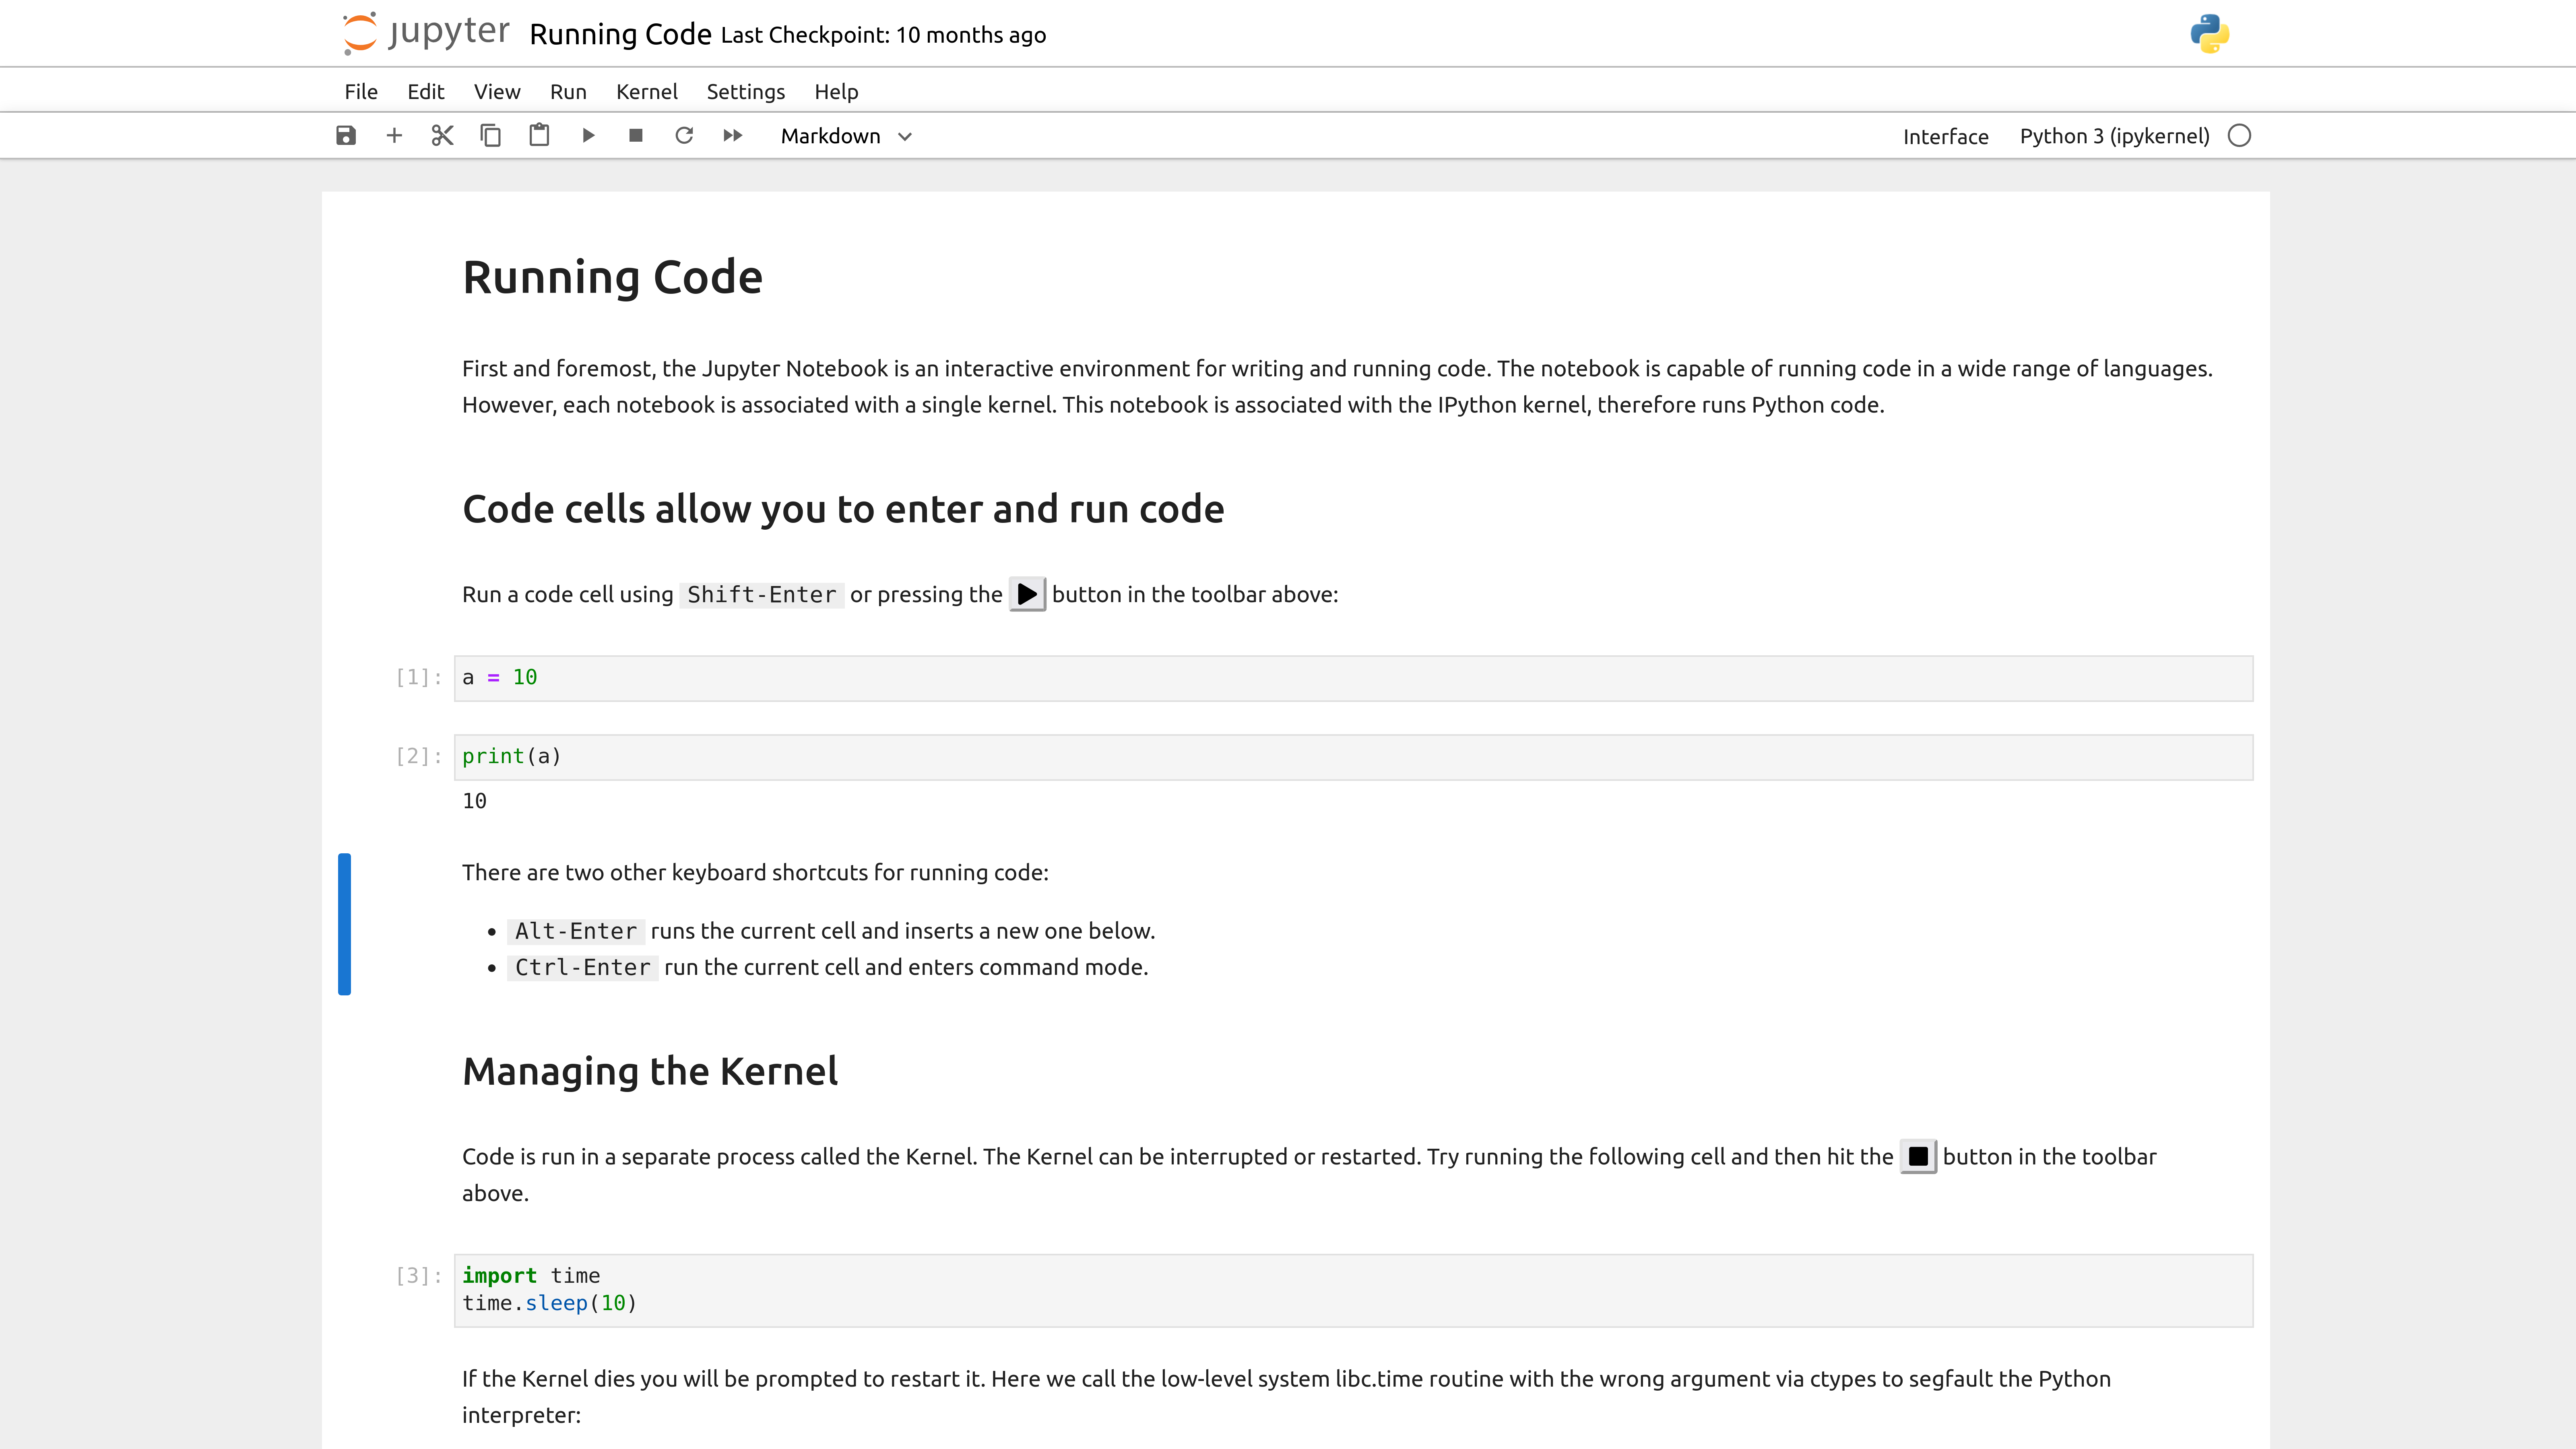
\includegraphics[width=1\textwidth]{figures/running_code.png}
	\label{fig:running_code}
\end{figure}

\subsubsection{The Value of Jupyter Notebooks}
There are several advantages of Jupyter Notebooks: sharable, all-in-one, and 
live code. First of all, the notebook is easy to share because it can be 
converted into other formats such as HTML, Markdown, and PDF. This is 
advantageuous because it allows someone working on a notebook to share it with 
others without requesting that they install any additional software and making 
it easier to collaborate on the projects. Secondly, Jupyter Notebooks combine 
all aspects of data in one single document, making the document easy to 
visualize, maintain and modify. In addition, they provide an environment of 
live code and computational equations. Usually, when programmers are running 
code on some other IDEs, they have to write the entire program before executing 
it. However, the notebook allows programmers to execute a specific portion of 
the code without running the whole program. The ability to run a snippet of 
code and integrate with text highlight the usability of the notebook. Previous 
research has demonstrated that Jupyter Notebooks can significantly contribute 
to reproducibility, reusability, and more effective computational workflows in 
science \cite{beg2021using}.

\section{Problem Statement}
Since both Jupyter Notebook and Drasil focus on creating and generating 
scientific computing documentation, we are interested in extending the values 
of Jupyter Notebook to Drasil and the kind of knowledge we can manipulate. 
Following are the three main problems we are trying to solve with Drasil in 
this paper:

\begin{enumerate}
	\item Generate Jupyter Notebooks. To acheive this, we will have 
	to generate documents in notebook format. Jupyter Notebook is a simple 
	JSON document with a .ipynb file extension. Notebook contents are either 
	code or Markdown. Therefore, non-code contents must be in Markdown format 
	with JSON layout. Drasil can currently write in HTML and LaTeX. We are 
	building a notebook printer in Drasil for generating documents that are 
	readable and writable in Jupyter Notebook.
	\item Develop the structure of lesson plans and generate them. As 
	mentioned, Jupyter Notebook is used as an educational tool for teaching 
	engineering courses. When it comes to teaching, lesson plans are often 
	brought up because they help teachers to organize the daily activities 
	in each class time. We are interested in teaching Drasil a ``textbook" 
	structure by starting with generating a simple physics lesson plan and 
	expanding Drasil's application. We aim to capture the elements of 
	textbook chapters, identify the family of lesson plans, and classify the 
	knowledge to build a general structure in Drasil, which will enable the 
	lesson plan to generalize to a variety of lessons.
	\item Generate notebooks that mix text and Python code. Jupyter Notebook is 
	an interactive application for creating documents that contain formattable 
	text and executable code. However, Drasil doesn't currently support 
	interactive recipes. There is no code in SRS documents, and text and code 
	are generated separately in Drasil. We are looking for the possibility of 
	generating a notebook document that incorporate both text and Python code, 
	thereby	enhancing the capabilities of Drasil and its potential to solve 
	more scientific problems.
\end{enumerate}

\section{Thesis Outline}
Chapter~\ref{chap:nbprinter} covers the topic of how Drasil generates and 
prints documents using the Drasil printer, as well as the creation of the 
notebook printer for generating Jupyter Notebooks in Drasil. Moving on to 
Chapter~\ref{chap:lessonplan}, we discuss the structure of lesson plans, how we 
define the lesson plans language in Drasil, and how to generate them with the 
notebook printer. Chapter~\ref{chap:codeBlock} discusses various approaches for 
splitting the contents to mix different types of content, such as text and 
code, in Jupyter Notebooks with Drasil, as well as the implementation for 
generating code blocks. Lastly, Chapter~\ref{chap:conclusion} provides an 
overview of the future work and concludes the achievements of this work.
\chapter[Ideology]{Ideology\footnotemark}
\footnotetext{Or, at least, my understanding of a software development ideology
    I believe to be relevant to this work and Drasil.}
\label{chap:ideology}

``Generation'' is at the heart of this work. However, unlike GitHub and OpenAI's
Copilot \cite{Copilot}, we don't delve into artificial intelligence. Copilot
uses AI to autocomplete code using smaller snippets and comments, while we focus
on capturing the meaning of specific subsets of language to generate software
artifacts through description of their requirements. In other words, we focus on
encoding the important bits of information that we use to discuss requirements
of software and how they relate to the software artifacts we would normally
manually write. We focus on capturing knowledge through codifying
well-understood fragments with \acsp{dsl} to capture the \textit{harmonious
relationship} between \textit{knowledge} and \textit{software artifacts} to
improve software \textit{maintainability} and knowledge \textit{communication}
and \textit{reusability}.

\section{On Developing Software}
\label{chap:ideology:sec:on_developing_software}

As software developers, we encode ``stories'' through software. As an example,
programs made to process \acs{csv} files tell a story of how data can be
entered, adjusted, and output. Compilers tell a story of how human-readable
programs can translate to various assembly languages. In these stories, we
commonly use similar terminology and ideas. Thankfully, we avoid writing ``a lot
of the same code'' by abstracting over variables and sharing reusable code
through libraries. With libraries, we're able to share our knowledge with our
future selves and others alike. Once we've reasonably stabilized our libraries,
it becomes a large gain in the reusability of our efforts \textemdash we don't
need to worry about making the same bugs twice! However, a few issues arise: the
code might become out-of-date (or out-of-sync), others might not understand what
we wrote (and thus not trust/use it), or we might need to use the same
conceptual ideas but in a different programming language. If our understanding
of key ideas changes, we might need to perform large, manual refactoring of our
code, and also update our documentation too. While we might write ``idiomatic''
code, reverse engineering code is tedious, and even then, we can only analyze
the code we \textit{see}, and not what knowledge it took to write that code.
Finally, we might be able to write a \ACF{ffi}, but they're often brittle and
demanding of our time, due to initial and repeated complex analysis for each
library update. We might even be forced to use particular programming languages.

Often, we look to using mature libraries and frameworks to underpin our
projects, but usually without a guarantee that how we use and connect libraries
is ``safe.'' For example, the sinking of the Vasa ship \cite{wiki:Vasa_ship} was
partially caused by different teams working together but using different
``feet'' units (the Swedish foot is 12'' while the Amsterdam foot is 11'')
resulting in unbalanced weight distribution, contributing to its demise.
Similarly, when the Mars Climate Orbiter travelled to Mars, it met an early
demise due to a navigation issue \cite{Siddiqi2018}. Lockheed Martin built the
orbiter ground controller software, but it didn't conform to \acsp{nasa}
\ACF{sis}. The commands sent from Earth used English units (specifically,
pound-seconds) while the orbiter assumed that it would receive commands using
the metric system (Newton-seconds). As such, the orbiter missed its intended
target orbit altitude, falling into the Martian atmosphere, and ultimately
disintegrating due to atmospheric stress.

Experts had an in-depth understanding of the ``story'' of each project, with
sound rationale for how things worked and should have worked, and yet both
ended in misfortune. Of course, most software is not critical, and issues in
most software will not result in an orbiter disintegrating in Martian atmosphere
or a ship sinking, but there is something that we can learn:
\textit{communication} and \textit{synchronization} of development efforts is
vital for building reliable solutions.

While we as developers don't often build and connect physical things, we do
connect pieces of code\footnote{Though robotics is a field too.}, and
misunderstandings of tacit project knowledge occur too. Thus, we believe we need
to revisit our original sensation when we recognized code duplication and
decided to make reusable components.

The reason is obvious\footnote{Ignoring the more obvious reasons, such as
copy-pasting code, or mere awareness of textual similarities.}! We felt this
sensation because we already had a mental model that connected some key concepts
to some code we wrote, so we decided to make reusable views (code) of our
knowledge. However, the code is only a shallow view of our knowledge, containing
very little discussion of the conceptual underpinnings and the role they play in
the greater ``story.'' Shallow views of implicit, unwritten knowledge,
unfortunately, does not come with guarantee of harmony with the way it's used.

\section{Dreams of Generation}
\label{chap:ideology:sec:thoughts_of_generation}

Unlike the Vasa, for stories where the desired end-product somehow involves
software, we can remedy the communication issue partially by unifying it under
one cohesive story. \Acfp{srs} play a large role in unifying communication of
software needs. However, the communication and maintained synchronization of the
software requirements into the final software product is still brittle (as
evidenced by the Mars orbiter), as it remains heavily reliant on manual labour
to translate it into software artifacts. In other words, the translation from
our knowledge (the important part) is laborious and prone to error, and hence,
not simple enough. So, now we wonder: how can we simplify the process?

Our end-goal should be ``assembly-line'' style engineering of software
\cite{well-understood}, free of logical issues. To attain this, we need to have
clear criteria for what it means for our software artifacts to be free of
logical issues. However, to do this, we need to discuss relevant models. For
example, if we're interested in the accuracy of a bank accounts cached balance,
we discuss \textit{the user}, the relevant \textit{transactions}, and then a
\textit{validation algorithm}. Realizing this example in code might have us
retrieve a user's bank transactions, calculate the expected balance, and compare
it with a cached balance. The code only contains one dimension of this
discussion: the actions. It has no understanding of the substance, nor how it
can be similarly used in other scenarios. To audit the code, we analyze the code
ourselves, potentially with extra testing tools to make things quicker, but in
general, it relies on us and our understanding. To remedy this, we look to
describing software as we've done here: as a ``view'' of some story or
discussion. In other words, we want to build software artifacts through
description as opposed to manual conversion of description to artifact.

\subsection{The Goal}
\label{chap:ideology:sec:thoughts_of_generation:subsec:the_goal}

If we think of a Java compiler as a sort of \textit{generator} of \acs{jvm}
bytecode, we can think of the Java programs as the instructions and inputs to
the generator. We rarely look at the actual bytecode ourselves, but we do have
confidence in knowing what it will do when executed. Now, we look to go one
``level'' up. In other words, we look to inputting our understanding of
particular applications through another generator (an abstraction level up) to
somehow obtain code for it.

Especially in the cases where everything is ``well-understood''
\cite{well-understood}\footnote{Irrelevant of rarity!}, we want to focus on
communicating problems and how solutions solve them so that we can
\textit{generate} usable solutions (a software artifact), and keep them
up-to-date through re-generation.

\subsection{Reconciliation}
\label{chap:ideology:sec:thoughts_of_generation:subsec:reconciliation}

By focusing on capturing well-understood \cite{well-understood} knowledge, we
can use (and re-use) knowledge across specialized generators to generate
software for specific kinds of problems. For example, statisticians frequently
use and discuss various kinds of distributions, such as ``Poisson,''
``Uniform,'' and ``Normal,'' and when they do, they're typically familiar with
their parameters, expectations functions, and how to use them to estimate
likelihoods. Hence, by focusing on using \textit{\acsp{dsl}}, we can build
specialized interpreters for them. Furthermore, by connecting them in precise
manners (with similar precise languages), we can form large meaningful
\textit{networks of domains} \cite{Czarnecki2005} that form our well-understood
problem spaces. For well-understood problem spaces, we can compose a series of
domain-specific interpreters. With enough effort, we could take a whole
``problem description'' that draws in multiple fields, and generate software
that somehow ``solves'' it.

By switching our focus of manual software development to manual problem
description and relationships to ``solutions,'' we shift where we can make bugs,
and how they propagate. Namely, logical bugs will occur more than once so as
long as the same knowledge pulled from is drawn more than once. Thus, each
logical bug should be more visible and easier to spot. Additionally, the
generated software becomes directly \textit{traceable} to its logical
foundations. Hopefully, with adequate dissection of related concepts, bugs
should also be less intricate. Furthermore, generated artifacts are simpler to
\textit{maintain} (i.e., kept in synchronization) with its related
knowledge-base and story by \textit{regenerating} it. Finally, as opposed to
sharing \textit{code}, in this paradigm, we \textit{communicate knowledge},
achieving language-agnostic reusability, focusing on sharing meanings and
families of problems rather than solutions. Thus, by focusing on generating from
meaningful descriptions, we obtain \textit{knowledge reusability} (as opposed to
\textit{code} reusability), and increased software \textit{maintainability},
\textit{reliability}, and \textit{traceability}. Of course, generating all
software artifacts appears grandiose, and, perhaps, reductive or ignorant of
many difficulties in software development. Thus, we must discuss
feasibility\footnote{You may skip the remainder of this chapter if you so wish,
it is not strictly required to understand the rest of my work, but it doesn't
hurt.}.

\subsection{Feasibility}
\label{chap:ideology:sec:thoughts_of_generation:subsec:feasibility}

For us to discuss feasibility of this idealized development paradigm, we must
discuss the \textit{depth} and \textit{breadth} of knowledge we need to make
this feasible\footnote{Note that ``knowledge'' is captured through codifying
\acsp{dsl}.}. Depth of knowledge refers to the vertical knowledge understood
about a specific fragment of knowledge, and its preciseness. For example, we may
have a low-depth of knowledge and claim that English sentences are a sequence of
characters. Alternatively, we might have a slightly ``deeper''
depth/understanding  of sentences by describing them as a language that follows
a specific syntax rule set and using a specific set of words. Breadth of
knowledge is the horizontal domain of knowledge, it is the various kinds of
knowledge we have in a wide variety of subjects and domains.

\subsubsection{Low Depth \& Narrow Breadth}
\label{chap:ideology:sec:thoughts_of_generation:subsec:feasibility:subsubsec:low}

At a shallow depth and narrow breadth of knowledge capture, this paradigm is
very practical, and already heavily used. Widely used \ACFP{cms}, such as
WordPress \cite{WordPress} and Drupal \cite{Drupal}, and web frameworks, such as
Django \cite{Django} and Laravel \cite{Laravel}, are arguably also following
similar ideals as this ideology. Notably, they \textit{deeply embed}
\cite{Carette2009} knowledge in their frameworks and libraries using their host
programming languages basic features. They all typically provide a basic
understanding of ``user's'' of a hosted website, facilities to write \acs{html}
content in one way or another (e.g., \acs{wysiwyg} editors, templates, and
plugins). While some might be, these listed above are not specific to one
specific use-case. They're versatile products, usable for a wide variety of
use-cases because they ship with low but sufficient depth of
knowledge\footnote{They might call it ``features.''} such that you can use them
for a wide variety of different applications (e.g., blogging, ticketing,
booking, accounting, etc.). Out of the box, these web technologies listed come
with simple, common, functionality (features) and powerful extensibility through
either plugins or through software extension and usage. With the basic tooling
provided, users are able to rapidly deploy websites with content. Through
extending the website's knowledge-base (e.g., plugins or software extension),
they are able to obtain a wider breadth and deeper depth to the knowledge
contained within them. Through this, end-users may encode increasingly complex
and different kinds of data into the systems to ultimately obtain increasingly
specialized websites, such as technical blogs, eCommerce websites, online
accounting software, online discussion forums, and more.

The mechanized generation-related components of the ideology is also fairly
shallow in this area, but still, highly feasible. In some sense, almost any
individual instance of ``generation'' is an area of low depth and breadth as
well.

At the lowest depth and narrowest breadth of knowledge capture, we aren't really
capturing any meaning. Rather, we are programming our software artifacts
directly. Hence, this area is already very feasible, evidenced by the usefulness
of software in usage today, and the way said software was made.

\subsubsection{Specialized Tools: Deep Depth \& Narrow Breadth}
\label{chap:ideology:sec:thoughts_of_generation:subsec:feasibility:subsubsec:specialization}

We might think of software that captures deep knowledge about a specific topic
as \textit{specialized tools}. Tailored to specific needs, they come with extra
features for highly specific, potentially niche, categories of
problems\footnote{Think of this category as sharp tools, such as kitchen knives.
We can generally get away with using basic kitchen knives, but specialty knives
help us out for particular use-cases, such as serrated  or filleting
knives.}. These already exist, and are similar to the ``Bottom,'' highly
practical. For example, \ACFP{aml} (such as HashedExpression
\cite{HashedExpression}) allow you to describe complex mathematical algorithms
and generate optimized software tools for solving them. Another example is
parser generators (such as Happy \cite{Happy}). They capture complex information
about grammars and allow users to generate specialized parsers for them. When
needed, specialty tools provide greater functionality than general-purpose
programming languages for solving specific problems.

\subsubsection{Off-the-shelf Solutions: Low Depth \& Wide Breadth}
\label{chap:ideology:sec:thoughts_of_generation:subsec:feasibility:subsubsec:modelling}

Orthogonal to the ``specialized tools,'' a capture of low depth and wide breadth
of knowledge is seemingly a jack of all trades, master of none. For example,
most modern programming languages come with a standard library that provide many
off-the-shelf solutions to well-understood problems, but sticking to very common
generic problems. Most users typically pull in a library that provides extra
specialization for certain problems because the standard library didn't go deep
enough for their needs. Similar to the categories before, these are widely used
and similarly practical.

\subsubsection{Utopia: Deep Depth \& Wide Breadth}
\label{chap:ideology:sec:thoughts_of_generation:subsec:feasibility:subsubsec:utopia}

Finally, we've reached the category of ``deep depth and wide breadth'' of
knowledge capture. Here, we capture the meanings of key ideas and concepts we
need to build software, making as many conscious decisions explicit and visible
as possible. Imagine using the specialized tools to develop every aspect of some
software artifact, but for every facet of the artifact, from start to finish.
This is an idealized method of developing software, where knowledge is strongly
reusable and composable. Of course, this relies on heavy research on tooling. As
long as developers have infinite patience and can invest infinite time into
transcribing and researching to fill in gaps, anything is possible, and this
ideology is very practical! Unfortunately, that situation is not quite
realistic. As such, we should restrict our scope of captured knowledge to
``well-understood'' domains \cite{well-understood}. For areas of
``well-understood'' knowledge, this should be more feasible, merely because the
discussion of key ideas is already coherent and sufficiently codified.

Here, you might use a series of \acsp{dsl} to create a coherent discussion (a
``story''). With it, you would have specialized interpreters built, which
process it, and draw out meaningful byproducts you're interested in (such as
usable software). This story can be relatively far removed from produced
artifacts generating (containing potentially little to no discussion of the
desired artifacts at all), or a precise description (where you might be manually
writing out the final artifacts yourself). Through creating a story as a
composition of many other smaller fragments of knowledge and stories, and
defining interpreters as compositions of other, smaller interpreters, this is
feasible. Hopefully, with enough effort, this should alleviate considerable
stress associated with manual software development, by moving the focus to the
important bits: the story the artifacts tell. The ``quality'' of the generated
artifacts become a traceable reflection of the ``quality'' (depth and breadth)
of the captured knowledge.

\section{A Prospective Workflow}
\label{chap:ideology:sec:a_prospective_workflow}

In theory, all ``development'' should occur in a \ACF{kms}, where knowledge and
transformations between fragments of knowledge are transcribed. ``Users'' would
use a system of pre-filled knowledge to piece together a template story that
fits their narrative, or they would adapt an existing one to fit theirs.

Ideally, the workflow associated with building some product artifact will have
each knowledge/product owner (e.g., actual property ``\textit{owner}'',
developers, managers, designers, etc.) work on strictly the components that are
related to them, and nothing else. At the ``bottom'', the final end-user is
tasked merely with providing feedback that can improve the quality of the
artifact(s). They are the ones that have an issue that can be resolved with some
sort of software artifact. At the ``top,'' product owners designate a basic set
of requirements of the artifacts using a coherent \textit{formal description}.
Product designers/orchestrators will take the requirements and convert them into
a coherent \textit{story} for how the requirements may be translated into a
final product. The story builds on well-understood knowledge of various domains
encoded by domain experts. The product designer is tasked primarily with
translation, while the domain developers and product owners are tasked with
encoding knowledge and instances of knowledge, respectively.

Through product owners describing their requirements coherently (e.g., via some
formal language), completely non-technical product owners may, and will, still
be key figures in the production of the product.

As the stress load/burden becomes shared under this paradigm, the sum of the
parts should be less than the whole. In other words, the cumulative stress of
associated with creating the whole is greater than the approximate sum of each
individual's stress associated with focusing on their respective domain.

Following this ideology, there will be at least 3 key roles associated with
developing artifacts: the \textbf{knowledge encoder}, the \textbf{knowledge
user}, and the \textbf{end-user} of the produced software artifact.

\subsection{Knowledge Encoder (Domain Expert)}
\label{chap:ideology:sec:a_prospective_workflow:subsec:knowledge_encoder}

The knowledge encoder should be a master of a particular domain. They are
expected to encode the knowledge discussed in their respective domain in such a
way that is accessible to those without knowledge of their domain. Additionally,
they should encode information about the ways in which the knowledge can be
transformed into other forms of knowledge (including that which is
interdisciplinary). The knowledge they would be encoding should be as well-known
and globally standardized as possible. As discussed in
\Cref{chap:ideology:sec:thoughts_of_generation:subsec:reconciliation}, it is
likely that the knowledge encoder will focus on writing a series of highly
specific \acsp{dsl}, where the languages may be restricted to as specific as one
term or a handful.

As a domain expert transcribing knowledge encodings of some well-understood
domain, one will largely be discussing the ways in which pieces of knowledge are
\textit{constructed} and \textit{relate to each other}. For the abstract
knowledge encodings to be \textit{usable} in some way, it is vital to have
``names'' (\textit{types}) for the knowledge encodings. In working to capture
the working knowledge of a domain, it's of utmost importance to ensure that all
``instances'' of your ``names'' (types) are \textit{always} usable in some
meaningful way and that the knowledge is exposed in a usable way (e.g.,
sufficiently through some sort of \acs{api}). In other words, all knowledge
encodings should create a stringent, explicit set of rules for which all
``instances'' should conform to, and, arguably, also creates a justification for
the need to create that particular knowledge/data type. As such, optimally, a
domain expert would write their knowledge encodings and renderers in a general
purpose programming language with a sound type system (e.g., Haskell
\cite{Haskell2010}, Agda \cite{Norell2007}, etc.) \textemdash{} preferring ones
with a type system based on formal type theories for their feature richness.

\subsection{Knowledge / Domain User \& Orchestrator}
\label{chap:ideology:sec:a_prospective_workflow:subsec:knowledge_orchestrator}

The knowledge user/orchestrator is tasked with connecting the work of the domain
experts into ``plug-n-play'' stories (arguably, compilers for the end-users to
use). They should also have a working understanding of what the end-user needs,
and how the needs relate to domains of knowledge. As such, they should be able
to encode and reduce friction between knowledge encoded by domain experts and
the goals of product owners.

\subsection{End-user}
\label{chap:ideology:sec:a_prospective_workflow:subsec:end_user}

The final end-user should find the most delight from this ideology. They are the
actual users of the software artifacts, perhaps tweaking the final build of the
software artifacts to be accustomed to their workflow. If the tasks assigned to
the knowledge encoders and the knowledge users are performed correctly, then the
end-user should have strong confidence in the artifacts as they were built with
strict adherence to the knowledge captured at \textit{every step of the way}. As
such, one should confidently expect the final software artifacts to be
completely devoid of unexpected things (including errors, unconformities to
specifications, etc.).

Any of the three (3) user types may use the ``plug-n-play'' stories to describe
problems and generate solutions based on them.

\section{Drasil}
\label{chap:ideology:sec:drasil}

To my understanding, Drasil \cite{Drasil2021} explores this ideology, focusing
on generating scientific software from user-described scientific problems using
Drasil-understood terminology (i.e., ones that a scientific domain expert
previously encoded).

\chapter{Drasil}
\label{chap:drasil}

\begin{writingdirectives}

      \item What is Drasil?
      \begin{enumerate}
            \item What does it do?
            \item Where can we find information about it?
            \item What are its successes?
      \end{enumerate}

      \item How does Drasil work?
      \begin{enumerate}
            \item SRS? Generation?
            \item Specifically, what are its current problems?
      \end{enumerate}

\end{writingdirectives}

In this chapter, we will discuss the project this work contributes to, Drasil.
Specifically, we will discuss at a high-level what Drasil is capable of, and how
it works.

\drasilLogoImg{}

\section{What is it? What can it do?}
\label{chap:drasil:sec:what-is-it-what-can-it-do}

Principally investigated by \porthref{Dr.\ Jacques
      Carette}{https://www.cas.mcmaster.ca/~carette/} and \porthref{Dr.\ Spencer
      Smith}{https://www.cas.mcmaster.ca/~smiths/},
\porthref{Drasil}{https://jacquescarette.github.io/Drasil/} is a software suite
for generating software for well-understood problems through a knowledge-first
approach \cite{Drasil2021}. Drasil captures the background knowledge involved
with software development to make it \textit{reusable}, improve
\textit{maintainability} of software, and strengthen \textit{traceability}
between desired ``software artifacts''\footnote{``Software artifacts'' being any
      file with a well-defined structure, such as plaintext files, Python code,
      \LaTeX{} code, \acs{html}, or \acs{json}.} and the background knowledge
\cite{SzymczakEtAl2016}. Currently, Drasil focuses on generating software
artifacts for \ACF{scs}, where it has been shown to improve software qualities,
such as \textit{verifiability}, \textit{reliability}, and \textit{usability}
\cite{Smith2018}.

\caseStudiesTable{}

Drasil's knowledge-capture approach to software development allows users to
remove themselves from the discussion of ``code'' and focus on the important
bits: the problem the code solves and how ``code'' ultimately relates to
it\footnote{Drasil allows users to ``keep at a safe distance'' from software,
but only so far as Drasil has encoded the terminology the users rely on for
conveying their problem to Drasil.}. Drasil's development is navigated through a
series of case studies: \refCaseStudiesTable{}. Each case study has users input
scientific problems using \acsp{dsl} that build up an abstract \ACF{srs}
\cite{SmithAndLai2005}. The \acs{srs} decomposes scientific problems into small
structured fragments of knowledge that have direct relations to ``code'' and can
be used flexibly as part of code generation. Through abstracting sufficient
depth and breadth of the knowledge in an \acs{srs} (e.g., including the inputs,
outputs, and calculation scheme), Drasil is able to generate software artifacts
that satisfy the designated \acs{srs}\footnote{It is helpful to think of the
\acs{srs} as a sort of ``recipe'' that Drasil follows to navigate the
generation.} (\refCaseStudiesCodeTable{}). Drasil relies on the capture of a
\textit{network of domains} \cite{Czarnecki2005} to generate artifacts. Roughly,
the network of domains related to the code generated related to an abstracted
\acs{srs} is as per \refRoughNetworkOfDomains{}\footnote{Note that this is not
representative of all knowledge captured in Drasil, but only that which is
relevant to generating code for a given \acs{srs} abstraction.}, where nodes are
the major categories of domains\footnote{In other words, each node contains its
own subdomain as well} and arrows are mappings between them. The current network
is built according to the needs of Drasil's case studies. One notable success of
the knowledge capture is the reusability of it to regenerate artifacts in
different, but similarly applicable, languages. For example, the \acs{glassbr}
case study had \porthref{software
artifacts}{https://github.com/smiths/caseStudies/tree/master/CaseStudies/glass}
manually built. Once the knowledge was codified in Drasil, the same knowledge
allows re-creation in \porthref{other
languages}{https://github.com/JacquesCarette/Drasil/tree/master/code/stable/glassbr}.

\roughNetworkOfDomains{}

Drasil is able to generate a host of \ACF{oo} programming language source codes
through compiling to \ACF{gool} \cite{Carette2019,MacLachlan2020}, which
compiles to several \acs{oo} languages (such as Java, Python, C/C$++$, C\#, and
Swift\footnote{Note that Swift was not discussed in \cite{MacLachlan2020}, but
      the renderer was built by Brooks as well.}). Drasil also contains renderers for
printing \acs{html} files, Makefiles, basic Markdown (enough for ``READMEs''),
GraphViz DOT \cite{Gansner1993} diagrams, and plaintext, \LaTeX{} documents.
\acs{srs} abstractions are renderable in either \LaTeX{} or \acs{html}.

\caseStudiesCodeTable{}

\section{How does it work? How is it used?}
\label{chap:drasil:sec:how-does-it-work-how-is-it-used}

As mentioned in \Cref{chap:drasil:sec:what-is-it-what-can-it-do}, Drasil relies
on building a tree of knowledge that contains sufficient information such that
software artifacts can be ``grown'' from them. The individual pieces of
knowledge are known as \textit{chunks} and are encoded as either \ACFP{adt} or
\ACFP{gadt}. Drasil, and all knowledge captured in Drasil, is deeply embedded in
Haskell \cite{Haskell2010} \porthref{source
      code}{https://github.com/JacquesCarette/Drasil/}\footnote{The source code
      compiles against \acs{ghc} 8.8.4 \cite{GHC884} and uses \acs{ghc} language
      extensions.}. Each chunk has a \textit{type} which defines its structural
information. Chunks contain information encoded with various \ACFP{dsl}. The
network of domains (roughly, \refRoughNetworkOfDomains{}) is made up of a series
of chunks connecting and discussing one another, similar to how we might discuss
abstract concepts.

The ``coherent \acs{srs} abstraction'' of \refRoughNetworkOfDomains{} is
modelled after the \textit{Smith et al.} formal \acs{srs} template
\cite{SmithAndLai2005}, while the ``scientific knowledge'' higher up is a set of
interconnected chunks (and, hence, \acsp{dsl}). The ``scientific knowledge''
chunks are used to fill in the ``gaps'' of the \acs{srs} template. For example,
if we wanted to encode a variable, \(\hat{q}_{\text{tol}}\), representing a real
number, ``Tolerable load,'' we might write it as
\refOriginalQuantityDictExampleHaskell{}, where it is of type \QuantityDict{}
(\refOriginalQuantityDictHaskell{}\footnote{Note that \IdeaDict{}, \Space{},
\Symbol{} (for all \Stage{}s), and \UnitDefn{} are coupled together to create
the quantity. The components respectively define the term, type, symbol
(dependent on the usage context [equational or software implementation]), and
unit of the quantity.}), the type of variable encodings.

\originalQuantityDictExampleHaskell{}

\originalQuantityDictHaskell{}

Notably, in \refOriginalQuantityDictExampleHaskell{}, the symbol,
\(\hat{q}_{\text{tol}}\), is built using a \Symbol{} \acs{dsl}. The capture of
domain-specific knowledge is what sets \acsp{dsl} apart from general-purpose
programming languages. Domain-specific abstractions create opportunities for
domain-specific \textit{interpretation and transformation} (e.g., optimization,
analysis, error checking, tool support, etc.) \cite{Czarnecki2005}. For example,
with the symbol for ``tolerable load,'' we have information about the structure
of the symbol itself: that ``q'' has a ``hat'' and a subscript ``tol.'' From
this, we can output the same information in alternative flavours if we desired,
such as plain text, or with Java-compatible naming convention (e.g.,
``qHatTol'').

Drasil's \acs{srs} template contains more ``holes''\footnote{Or ``blanks'' if you
      think of the template as a ``fill-in-the-blanks'' puzzle.} for other
information necessary to creating a whole ``story'' about how
\textit{output variables} can be calculated according to a set of
\textit{input variables} and algorithm derived through a series of
\textit{theories}. With sufficient knowledge \textit{depth}\footnote{Note
      that the \acs{srs} template provides the \textit{breadth} needed by
      design!} for each relevant fragment, Drasil is able to automatically
``check'' it for consistency and coherence, and generate representational
code\footnote{``Representational code'' meaning software that solves the
      problem the related \acs{srs} abstraction describes, using the algorithm
      outlined.}.

Unfortunately, not all of Drasil's case studies are capable of generating
representational code (\refCaseStudiesCodeTable{}). Some case studies
(\acs{gamephysics}, \acs{hghc}, and \acs{ssp}) are still actively being
developed, but are left incomplete at the time of writing. \acs{nopcm} is usable
in all languages supported by \acs{gool} except for Swift due to the lack of a
Drasil-supported \acs{ode} solving library for the Swift \acs{gool} renderer.
\acs{pdcontroller} was built \cite{DrasilPR2289Naveen} outside the normal means
of Drasil's case study development. Code generation for \acs{pdcontroller} is
not impossible (it's done for Python), it just requires more investigation by a
domain expert for the needs of compiling to more languages. However, both the
issues related to \acs{nopcm} and \acs{pdcontroller} are outside the scope of
this work. In this work, we will focus on a critical common denominator between
all examples: capturing mathematical knowledge for reliable \acs{srs} artifact
generation. In particular, we will focus on 2 primary aspects of mathematical
knowledge: the \textit{theories} and the \textit{expressions}.

\chapter{Theories}
\label{chap:modelkinds}

\begin{writingdirectives}
    \item What are theories used for in Drasil?
    \item How are they captured in Drasil?
    \item Current problems? Solution?
\end{writingdirectives}

In this chapter, we will focus on improving inspection and interpretation
capabilities of theories in Drasil. Specifically, with focus on interpreting
them for generating software artifacts.

\section{Transforming Theories to Code}
\label{chap:modelkinds:sec:transforming-theories-to-code}

As already mentioned in \Cref{chap:drasil}, the \acs{srs} template
\cite{SmithAndLai2005} breaks up software requirements and problems into a
series of well-understood components, providing developers with concrete
solution requirements they must satisfy, and domain experts with justification
for problem solutions. Notably, the \acs{srs} relates a programs \textit{inputs}
to a set of \textit{outputs} using a set of \textit{theories}. The inputs and
outputs are sets of variables, with data that need to be somehow fed into the
program, or calculated and output by the program. The theories connect the input
variables to the output by forming a \textit{solution/calculation path}.
Notably, the \ACF{im} \cite{SmithAndLai2005} theories together largely form the
calculation path, while other background theories provide justification for
them.

\subsection{An Example}
\label{chap:modelkinds:sec:transforming-theories-to-code:subsec:an-example}

For example, Drasil's \porthref{\acs{projectile} case
    study}{https://jacquescarette.github.io/Drasil/examples/projectile/SRS/srs/Projectile_SRS.html}
describes how to estimate if a launcher, aligned at a particular angle, will hit
a target from a specific distance. The \acs{srs} requires users to fill in the:
\begin{enumerate}
    \item input variables:
          \begin{enumerate}
              \item \(p_\mathit{target}\), the targets distance from the
                    launcher,
              \item \(v_\mathit{launch}\), the projectile launch speed,
              \item and \(\theta\), the launch angle.
          \end{enumerate}
    \item output variables:
          \begin{enumerate}
              \item \(s\), a message, explaining if the projectile hit the
                    target, fell short, or went long,
              \item and \(d_\mathit{offset}\), the expected distance between the
                    target position and the landing position.
          \end{enumerate}
    \item and theories, connecting the inputs to the outputs:
          \begin{enumerate}
              \item \({t_{\text{flight}}}=\frac{2 {v_{\text{launch}}}
                        \sin\left(\theta{}\right)}{\mathbf{g}}\), estimating
                    flight time with \(v_{\mathit{launch}}\) and \(\theta\),
              \item \({p_{\text{land}}}=\frac{2 {v_{\text{launch}}}^{2}
                        \sin\left(\theta{}\right)
                        \cos\left(\theta{}\right)}{\mathbf{g}}\), a calculation
                    of the landing position,
              \item \({d_{\text{offset}}}={p_{\text{land}}}-{p_{\text{target}}}\),
                    calculation of distance between the targets position and the
                    expected landing position of the projectile,
              \item and \(s=\begin{cases} \text{``The target was hit.''},        &
              |\frac{{d_{\text{offset}}}}{{p_{\text{target}}}}| < \varepsilon{}
              \\
              \text{``The projectile fell short.''}, & {d_{\text{offset}}} < 0 \\
              \text{``The projectile went long.''},  & {d_{\text{offset}}} >
              0\end{cases}\), \newline{}calculating the output message.
          \end{enumerate}
\end{enumerate}

From these 3 key bodies of information along with some supporting background
knowledge (such as assumptions, constants, etc.), Drasil forms a calculation
path, deriving the output variables from the input variables using the concrete
theories\footnote{The ``concrete theories'' are the ``instanced model'' and
    ``data definitions'' \cite{SmithAndLai2005} encodings (respectively,
    \InstanceModel{}s and \DataDefinition{}s) which are somehow usable in the
    solution of a scientific problem.}. Together, the theories form a calculation
algorithm which Drasil generates representational code of. For example,
\acsp{projectile} generates \refOriginalJavaProjectileMain{} for one of the
Java-flavoured artifacts. In \refOriginalJavaProjectileMain{}, it uses a
\inlineCode{java}{write_output} method to output the calculated output variables
after calculating them using the relevant theories\footnote{Note:
    \(t_\text{flight}\) is seemingly unused in the generated code, but it is used in
    the derivation of \(p_\text{land}\). However, it being ``unused'' is irrelevant
    to this work.}.

\originalJavaProjectileMain{}

As seen in \refOriginalJavaProjectileMain{}, it relies on a few methods
calculating the related ``instance models'' on its behalf. Those methods are a
specific \textit{interpretation}\footnote{Or ``view.''} of the theory knowledge.
Specifically, it is a \textit{calculation-focused} interpretation. For example,
to calculate \(p_\text{land}\), \refOriginalJavaProjectileMain{} relies on the
method \inlineCode{java}{func_p_land} to calculate the landing position.
\refOriginalJavaProjectilePLandMethod{} is one possible exported method for
calculating \(p_\text{land}\) given \(v_\text{launch}\), \(\theta\), and
\(\mathbf{g}\).

\originalJavaProjectilePLandMethod{}

Of course, to generate this method in \refOriginalJavaProjectilePLandMethod{},
Drasil relies on a sufficient capture of its underlying knowledge, and a means
of transforming said knowledge to ``code'' (e.g., sufficient information that
answers: What do we want to define? How can it be converted to code?). This
capture of theories is done using Drasil's representation of an ``Instance
Model.'' To build it, Drasil uses information gathered from what users fed in
about it, via \refOriginalLandPosTheoryDefinition{}.

\originalLandPosTheoryDefinition{}

Now, let's unpack \refOriginalLandPosTheoryDefinition{}. \inlineHs{landPosIM} is
an instance of an \InstanceModel{}\footnote{Drasil's encoding of the ``Instance
    Models.''}, containing the equational definition component
(\inlineHs{landPosRC}), and meta-level information about the theory, including
constraint ranges, notes, and a derivation\footnote{Mostly omitted here for the
    sake of conserving space.}.

To transform \refOriginalLandPosTheoryDefinition{} into
\refOriginalJavaProjectilePLandMethod{}, \textit{interpretation}\footnote{More
    accurately, this interpretation is ``domain-specific interpretation''
    \cite{Czarnecki2005}.} occurs on \inlineHs{landPosRC}
(\refOriginalRelToQDHaskell{}).

\originalRelToQDHaskell{}

\refOriginalRelToQDHaskell{} shows the definition of \relToQD{}, a function that
attempts to convert arbitrary relations into coherent ``quantity
definitions''\footnote{Or, ``variable definitions.''} (\QDefinition{}), which
Drasil's ``\acs{srs} to code'' generator relies on. \inlineHs{landPosRC} is an
instance of a \RelationConcept{} (\refOriginalRelationConcept{}), a coupled
mathematical relation (encoded using \Relation{}s\footnote{\Relation{} is
    Drasil's \acs{dsl} encoding arbitrary mathematical relations. We will talk more
    about this later. For now, this is enough.}), natural language description of
the relation, and descriptive name.

\originalRelationConcept{}

\relToQD{} is used on \textit{all} of the captured \InstanceModel{}s of a case
study to find code it can generate. However, these \InstanceModel{}s carry
arbitrary \Relation{}s, which are arbitrary mathematical relations. As such, an
issue arises: since \relToQD{} only works with ``variable defining''
relations\footnote{In some sense, calling these relations ``variable defining''
    is also an issue of itself. We're overloading \(=\) to mean definition.}, we're
limited to only one \textit{kind} of theory. Even with this restriction, we're
further limited to only a specific formation of that theory (e.g., relations of
the form \(x = f(a, b, c, \ldots{})\))!

\subsection{Problems}
\label{chap:modelkinds:sec:transforming-theories-to-code:subsec:problems}

In the sense that we really want to be able to use \relToQD{} (or something like
it) to transform arbitrary well-understood \textit{theories} into code fragments
for Drasil's code generator, it has at least 3 problems:
\begin{enumerate}
    \item[\namedlabel{mk:issue:1}{P1}] it only handles one theory kind:
        variable definitions,
    \item[\namedlabel{mk:issue:2}{P2}] and for those definitions, it requires a
        specific form, thereby limiting users to very specific usage, views, and
        transcription,
    \item[\namedlabel{mk:issue:3}{P3}] and it implicitly assumes that all inputs
        will be of this theory kind, or else it causes a panic.
\end{enumerate}

As a result of \ref{mk:issue:1}, we aren't able to encode adequately all the
theories we're interested in using, and want to generate representational code
of. In particular, as Drasil is heavily guided by physics-focused case studies,
\acsp{ode} are desired! When we want to use \acsp{ode} in the solution of a
problem, extra information is required. For example, we might need to give
Drasil (and/or developers) information about a desired approximation formula
with particular ``settings.'' Drasil does circumvent this issue for \acsp{ode},
but we would like to reconcile the half-measures and push all necessary
information back in to the theory encodings.

Assuming we wanted to describe the theory of a line, there are many ways we can
describe the equation: polynomial (\(ax + by + c = 0\)), slope-intercept form
(\(y = mx + b\)), point-slope form (\(y_1 - y_2 = m(x_1 - x_2)\)), and so on.
However, as a result of \ref{mk:issue:2}, we are forced to use the ``simple''
slope-intercept form, even though we are aware of other forms and may prefer to
describe it in other forms.

As a result of \ref{mk:issue:3}, when Drasil's users are encoding theories in
Drasil, they might be misled to think that any of their encoded theories is
fully-understood to Drasil and actually usable as part of the generated solution.

Together, these issues arise because of a lack of sufficient \textit{depth} and
\textit{breadth} in the contained knowledge of the theory encodings. Because the
theory encodings rely on ``flat'' information (e.g., the relations),
transforming them programmatically is challenging. Of course, if two programmers
were to read this information in the \acs{srs}, they might be able to use it.
However, the programmers understand the context of the theory, and are able to
\textit{recognize} (from any form of a theory) if and how it can be transcribed
as a computation. Now, imagine if we wanted to  So, how can we mitigate all of
these issues?

Just as we may discuss the specifics of implementing any particular theory in
our manual implementation of a software artifact, we assume prior learned
knowledge about mathematical expressions, such as which ones we know we can
somehow translate into code. To mitigate these issues, we must further capture
this background knowledge because raw relations carry too little information
about how to transform into coded. So, now, more concretely, we ask: how could
we have avoided these individual problems?

\begin{longtable}[c]{>{\raggedright}p{0.2\linewidth}>{\raggedright\arraybackslash}p{0.65\linewidth}}
    \textit{To avoid~\ldots{}} & \textit{we needed~\ldots{}}                                    \\
    \ref{mk:issue:1}           & knowledge about more \textit{kinds} of theories,               \\
    \ref{mk:issue:2}           & to decompose the relations into its set of
    logical components and capture information about how instances can be
    transformed into various forms,                                                             \\
    \ref{mk:issue:3}           & a signifier for each theory \textit{kind} we're interested in. \\
\end{longtable}

Succinctly, this means we need a system for \textit{classifying} and
capturing/exposing the \textit{structure} of more \textit{kinds} of theories.
This also means \RelationConcept{}s and \Relation{}s are insufficient couriers
of ``theory knowledge.'' In particular, we should be careful to ensure that the
abstractions are capable of reproducing the original knowledge we abstracted
them out of\footnote{This also should typically create opportunity for more
    kinds of interpretation of the abstracted knowledge too.}. In other words, we
should ensure that we can re-create the original \RelationConcept{}s from the
newly created, structured, theories.

\section{Classifying Theories}
\label{chap:modelkinds:sec:classifying-theories}

As a result of the inability to enter in complex theories not of the form \(x =
f(a, b, c, \ldots{})\) and the desire to encode theories with
\acsp{ode}\footnote{As Drasil's examples are physics-focused and \acsp{ode} are
    common in physics problems, the ability to generate software that can solve
    \acsp{ode} is desired.}, Drasil's existing \acsp{ode} has a bit of temporary code
to circumvent the ``1 Theory Kind'' restriction. However, we won't focus on
\acsp{ode} in this work. Since we only have one kind of theory that is processed
down the ``normal'' route (\relToQD{}) along the path of code generation, we
will focus on it.

Continuing to use \(p_\text{land}\) as an example, recall
\refOriginalLandPosTheoryDefinition{}, as it is similar to any one of the other
theories in Drasil used for code generation (other than \acsp{ode}!). The code
generator currently understands how to convert ``quantity definitions''
(\QDefinition{}s, \refOriginalQDefinitionHaskell{}) into various snippets of
usable code that it can use to generate a whole software artifact.

\originalQDefinitionHaskell{}

\QDefinition{}s are ``higher-level'' versions of the existing theories. A
\QDefinition{} breaks up an equational theory (i.e., theories of the form \(x =
f(a, b, c, \ldots{}\)) into its logical constituents:
\begin{enumerate}
    \item a variable to be defined,
    \item an expression (formula) defining the variable,
    \item and a natural language explanation of the coupling.
\end{enumerate}

For our current needs, this is a sufficient interpretation of ``equational
theories.'' Additionally, since all existing instance models are processed by
\relToQD{}, we similarly have a clear path to converting the existing
\RelationConcept{}s into \QDefinition{}s where applicable. Specifically, to
convert them, we merely need to hand-process \relToQD{} in the case studies,
where we normally write \RelationConcept{}s\footnote{Note: since the
    \QDefinition{}s are merely unpacked copies of the existing \RelationConcept{}s
    used in code generation, we can also similarly re-create those
    \RelationConcept{}s we're aiming to replace. In other words, we can also make
    \RelationConcept{}s a ``view'' of \QDefinition{} by re-interpreting them while
    connecting the formula to the defined variable with an equality.}. For example,
if we wanted to convert \inlineHs{landPosRC} into a \QDefinition, we might do it
as \refCurrentLandPosRCtoQD{}, where \inlineHs{E.landPosExpr} is a variable
containing the expression (formula) defining the \inlineHs{landPos} symbol.

\currentLandPosRCtoQD{}

However, merely replacing all \RelationConcept{}s with \QDefinition{}s is also
limiting. We want to use more \textit{kinds} of theories too! Thus,
\ModelKinds{} \footnote{\ModelKinds{} is based on a prototype by Dr.\ Jacques
    Carette. Shortly after implementing it, the Drasil Research Team discussed
    changing the name of ``models'' to ``theories,'' to which, we did, but have not
    propagated through the Drasil codebase, pending analysis on how it might affect
    the \acs{srs} template \cite{DrasilIssue2599RenamingModels}. Thus,
    ``\ModelKinds{}'' might change to ``\TheoryKinds{}'' or the singular
    ``\TheoryKind{}.''} (\refOriginalNewModelKindsHaskell{}) is created and
propagated through the various theory encodings to replace \RelationConcept{}s
(and \Relation{}s).

\originalNewModelKindsHaskell{}

\ModelKinds{} is an \ACF{adt}, enumerating over all currently
known\footnote{Criteria for ``currently known'' being ``ones this work has
discussed up until this point.''} \textit{kinds} of theories in Drasil. The
constructors of \ModelKinds{} are intended to carry structured encodings of
theory knowledge. By switching to \ModelKinds{}, theories can be created using
the structural information of theories, and the theories using structured
encodings are easier to refine and interpret\footnote{Such as for code
generation!} than the unstructured copies. At the moment, \ModelKinds{} has 3
kinds of ``models'' (theories) that can be created:

\begin{enumerate}
    \item \EquationalModel{}s, for theories that define a variable with some
          expression
    \item \DEModel{}s, for theories involve \acsp{ode},
    \item and \OthModel{}s, for everything else.
\end{enumerate}

Now, with \EquationalModel{}, we may finally rebuild \inlineHs{landPosIM}
(\refOriginalLandPosTheoryDefinition{}) using the improved structure
(\refCurrentLandPosIMQD{}). At the moment, it does not change the expected
generated artifacts, however, if desired, one can change output types of
theories in the \acs{srs} (or code) by adding new kinds of \QDefinition{} and
\ModelKinds{} interpretations.

\currentLandPosIMQD{}

Continuing, the \DEModel{}s still require a bit of manual circumvention, but
bringing some of the information back into the core ``theories'' to use in the
intended flow of knowledge, should be possible \cite{Chen2022MEng}. Drasil also
currently has many more kinds of theories, not all usable in code generation
\textemdash{} more than just equational models! However, we won't focus on them
\textit{quite yet}, we'll get back to this \Cref{chap:more-theory-kinds}.

Finally, as a result of incorporating \ModelKinds{} in Drasil, we:
\begin{enumerate}[label={(\alph*)}]
    \item add a system of classifying theories (through type information and
          constructors),
    \item change how users enter theories in Drasil (by making them enter in the
          structural components into ``cookie cutter'' shapes),
    \item gain information about theory capabilities (based on type
          information).
    \item and, ultimately, don't need \relToQD{} anymore.
\end{enumerate}

Now, on the note of exposing theory capabilities, we mean that we know have
static type information, at the level of the whole Haskell code compilation,
about how theories can be used. For example, if we previously had a function
that converts \RelationConcept{}s into pretty typeset boxes in \LaTeX{}, we
likely would have had similar troubles (as discussed above) in adding an
alternative printing form of the theory. However, now, we might, for example,
create a sub-kind of \EquationalModel{}s that are for equations of lines. Then
we can re-create the printing function for them, adding a parameter for the
printing form. The printing function now is able to more easily make use of the
logical constituents of a theory.

More important than printing to textual artifacts, we are interested in
generating code. Specifically, we are interested in knowing which
\EquationalModel{}s are usable in code generation, based on their defining
expressions.

\chapter{Expression Language Division}
\label{chap:lang-division}

\begin{writingdirectives}
    \item What are Relations really?
    \item What is \Expr{}?
    \item How is \Expr{} used?
    \item How can we restrict \Expr{} terms to particular areas?
\end{writingdirectives}

In this chapter, we will discuss how Drasil captures relations and general
mathematical expressions, and the issues associated with the single universal
language approach Drasil takes.

\section{Relations}
\label{chap:lang-division:sec:relations}

In \Cref{chap:modelkinds}, we discussed how Drasil captures theories.
Specifically, we discussed how Drasil heavily relies on relations for defining
them. However, we never discussed the relation encoding: \Relation{}.

\originalRelation{}

\Relation{} (\refOriginalRelation{}) is actually a type alias for \Expr{}
(\refOriginalExprHaskell{}), which captures general mathematical expressions. As
such, \Relation{}s aren't really ``relations.'' In fact, \Relation{}s can take
on any mathematical expression, such as \(3x+2\), which is obviously not a
``relation.''

\originalExprHaskell{}

\section{A Mathematical Language}
\label{chap:lang-division:sec:a-mathematical-language}

\Expr{} (\refOriginalExprHaskell{}) is an \acs{adt}\footnote{In \acs{gadt}
syntax.}, representing the \ACF{ast} of a mathematical expression language. It
was grown following the needs of encoding the case studies in Drasil. As such,
it contains a wide range of mathematical terms, including variables, numerics,
derivatives, common mathematical operations, and function applications. In
addition to the example expression (a relation) from
\refOriginalLandPosTheoryDefinition{}, if, for example, we wanted to transcribe
\(3 \tan{}(x) = y\) in Drasil, we might write \refPseudoExampleExpression{}.

\pseudoExampleExpression{}

Of course, this is great! We're able to transcribe any expression contained in
the language of \Expr{}. \refPseudoExampleExpression{} is a great example which
we can confidently re-write as an equational model (as in
\Cref{chap:modelkinds}):

\begin{pseudohaskell}{Example Expression in a QDefinition}{pseudoExampleExpressionAsQDefinition}
theQDef :: QDefinition
theQDef = mkQuantDef y (dbl 3 $* tan (sy x))
\end{pseudohaskell}

With \Cref{lst:pseudoExampleExpressionAsQDefinition}, we can create an instance
model containing an equational model as part of the solution of the greater
problem. One of the important requirements of instance models is that we expect
them to be unambiguously translatable into some component of the solution, up to
user choices (such as choosing what ``code'' representation of integers and
reals to use). This is where \Expr{} shows that it is a bit of a double-edged
sword. For example, we can re-write the expression used in
\Cref{lst:pseudoExampleExpressionAsQDefinition} using a trigonometric integral
(e.g., using \(\tan{}(x) + C = \int \frac{1}{\cos^2(x)}dx\) \cite{Math2Org}, we
obtain \(y = \int \frac{3}{\cos^2(x)}dx\) using \(C = 0\),
\Cref{lst:pseudoExampleExpressionAsQDefinitionBad}), but then the transformation
into a naive set of steps to follow isn't as simple.

\begin{pseudohaskell}{Example Bad Expression in a QDefinition}{pseudoExampleExpressionAsQDefinitionBad}
theQDef :: QDefinition
theQDef = mkQuantDef y (integAll (eqSymb x) (dbl 3 $/ (cos (x) $^ int 2)))
\end{pseudohaskell}

With \Cref{lst:pseudoExampleExpressionAsQDefinitionBad}, which solution to use
isn't clear. Should Drasil generate something to solve the integral? Should
Drasil replace the integral with the original $\tan$? How would it recognize to
convert it into $\tan$ without running into a similar problem as \relToQD{}
(\Cref{chap:modelkinds})? Should we expect the target generated languages to
have functionality for solving any integral we give it?

\textit{We} shouldn't be the ones answering any of these questions\footnote{We
should be imposing the least possible amount of things on users!}. Rather, we
should be deferring these questions to users, giving them options for choosing
answers to these questions. In other words, the transformation from \Expr{}s to
``code'' is not naively \textit{total}, which is problematic. However, these
questions are also still too complex to be external to the \acs{srs}, and as
such, we would need this theory to be a higher-level theory, which the user
refines with information that would appear in the \acs{srs} for domain-experts
to audit. In other words, we don't want integrals, like in this example, to
appear in the concrete theories (instance models) that are used in code
generation, at least without extra information about how to solve them embedded
closely.

Additionally, \Expr{} contains functionality for ``actors'' and ``messages,''
concepts in the world of \acs{oo} programming. While these are helpful for the
translation of mathematical expressions that might use some functionality from
``actors,'' users building an \acs{srs} should be relatively removed from the
actual programming. In other words, these terms are inappropriate for usage in
the \acs{srs}.

As such, we need to be able to restrict expression terms to their appropriate
contexts. At the moment, we lack information about when instances of expressions
are actually usable in code generation. As such, we're limited to relying on
implicit assumptions about this, and causing Drasil-panics when the assumption
is broken. To resolve this, we need to make the information \textit{explicit} in
Drasil, and use that explicit information appropriately. However, before we can
make it explicit, we need to understand the contexts in which Drasil needs
mathematical expressions and how they are used in those contexts.

Namely, there are at least three focal areas of interest in Drasil where we use
mathematical expressions:

\begin{enumerate}

    \item In the \acs{srs} for abstract theories, where we discuss abstract
          concepts that are ultimately used in the derivations of concrete
          theories,

    \item In the \acs{srs} for concrete theories (such as instance models),
          where we expect them to be \textit{concrete} in a sense that they are
          trivially usable as part of a solution to an outlined problem,

    \item In generated artifacts, where we first need to convert the
          concrete theories into an intermediate representation of the generated
          artifacts and making any necessary specializations for the target
          language, before finally outputting them.

\end{enumerate}

\section{Splitting}
\label{chap:lang-division:sec:splitting}

To restrict terms to their appropriate contexts, we need to somehow know when
users are using the ``wrong'' terms. Since Drasil is written in Haskell, we can
use Haskell's type system to indicate this with relative ease. Namely, we can
\textit{split} up \Expr{}. Thankfully, the three areas of interest share a
subset of expressions: the mathematical expressions usable in concrete theories.
As such, we would like to divide the language using this language as a base for
the other two (\refLanguageDivision{}).

\languageDivision{}

After the work, we end up with three languages:

\begin{enumerate}

    \item \Expr{}, which is the subset of the original \Expr{} where all terms
          have definite values (e.g., literals, common unary and binary
          operations, symbols, and first-order function applications), and
          should be the language of the \QDefinition{}s usable in instance
          models (\refCurrentExprHaskell{}),
    
    \item \CodeExpr{}, which is expected to be related to a \textit{total}
          transformation function that re-writes terms in \CodeExpr{} into
          \acs{gool} for final rendering in a final software artifact
          (\refCurrentCodeExprHaskell{}),

    \item  \ModelExpr{}, which is approximately the \Expr{} with nearly
          everything from the original \Expr{}, except without code-oriented
          terms\footnote{As they should not be discussed in the \acs{srs}
          documents at all!} (\refCurrentModelExprHaskell{}). Notably,
          \ModelExpr{} contains all indefinite valued terms that were cut out of
          \Expr{}, such as derivatives, integrals, quantification, types as
          values (spaces), and continuous ranges for summations and products.

\end{enumerate}

Now we have 3 \acsp{adt} available for different kinds of expression languages
with ``mathematics'' as a common tie. One issue with splitting is that we now
force users of the languages to make a conscious choice about which language
they are using, and which language they need to import into their working files
respectively. This can become quite frustrating given the amount of overlap.
Thus, to alleviate the stress involved with writing out the same expression in
different languages, we use a \ACF{ttf}~\cite{Carette2009} encoding of the smart
constructors to build expressions. Using \Expr{} has a ``base'' shared language
between \ModelExpr{} and \CodeExpr{}, we can write \acs{ttf} encoding for them
individually that extends on \Expr{}'s functionality
(\refCurrentExprTTFHaskell{}, \refCurrentModelExprTTFHaskell{},
\refCurrentCodeExprTTFHaskell{}). The \acs{ttf} encoding allows us to seamlessly
write expressions in any of the languages at the same time, allowing type
variability along the type constraints of any expression. The typeclasses used
in the languages may be used to create constriants on the language used.

While \ModelExpr{}s \acs{ttf} encoding strictly contains the terms unique to
\ModelExpr{}, it is possible (and typical) to convert \Expr{}s into
\ModelExpr{}s for usage in generating the \acs{srs} documents. Additionally,
since many theories need to be representable as a single \Relation{}, we may
create a typeclass to create enforcement (\refCurrentExpressHaskell{}). By
instantiating it for various types, we are explaining how those terms can be
interpreted as a \ModelExpr{}.

\currentExpressHaskell{}
 
\section{Back to Theories}
\label{chap:lang-division:sec:back-to-theories}

Now that we've split up the expression languages, we may restrict their usage to
appropriate theory contexts (in \ModelKinds{} as per \Cref{chap:modelkinds}).
Approximately, we can ``upgrade'' \ModelKinds{} according to
\refPseudoPartialModelKindsUpgrade{}\footnote{Note that we also need to slightly
update \QDefinition{}s: \refCurrentQDefinitionHaskell{} to create a type
parameter for the used expression type.}, creating a type argument in
\ModelKinds{} so that instance models can be restricted to carry ``\ModelKinds{}
\Expr{}'' while the other theory types may carry ``\ModelKinds{}
\ModelExpr{}''\footnote{However, using \Expr{} and \ModelExpr{} is not quite
accurately representative of ``usable in code'' versus ``not,'' which we are
going to fix \cite{DrasilIssue2853AlternativeModelKinds}.}. This allows us to
ensure that all expressions written in Drasil for instance models have an
semantic counterpart that they can be translated into for code generation in
various \acs{oo} languages. Furthermore, now we may return to \ModelKinds{} and
continue uncovering the various \textit{kinds} of theories currently discussed
in Drasil's case studies.

\pseudoPartialModelKindsUpgrade{}

\chapter{More Theory Kinds}
\label{chap:more-theory-kinds}

\begin{writingdirectives}
	\item What other theory kinds can we find in the existing Drasil examples?
	\item How is ModelKinds affected by the language division in
	\Cref{chap:lang-division}?
	\item What theories currently are used in Drasil?
\end{writingdirectives}

In this chapter, we return to examining more of the existing theories in Drasil,
and create alternative, structured versions of them to create further
opportunities for domain-specific interpretation.

\section{Remaining Theories}
\label{chap:more-theory-kinds:sec:remaining-theories}

As of writing, there are mainly two kinds of theories that are used in code
generation: the equational model and the \acs{ode} models. However, they aren't
the only kinds of theories encoded in Drasil. There are at least two other
re-occuring kinds of theories. One of them is a theory that shows multiple ways
to define a quantity. For example, \refExampleEquationalRealmImg{} is an example
from the \acs{dblpendulum} case study. Meanwhile, the other theory imposes
constraints on a system. For example, \refExampleEquationalConstraintsImg{} is
an example from the \acs{ssp} case study.

\refExampleEquationalRealmImg{} shows an abstract ``force'' variable,
\(\mathbf{F}\), which be defined by at least two different expressions: \(m
\mathbf{a}\) or \(-{\mathbf{T}_{1}}
\sin\left({\theta_{1}}\right)+{\mathbf{T}_{2}} \sin\left({\theta_{2}}\right)\).
This theory, in particular, is used abstractly, providing reasoning for building
different ways to define \(\mathbf{F}\), but also creating opportunity for
further specialization in other theories or systems. For example, this theory is
used as part of the derivation of another theory
(\refExampleEquationalRealmUsageImg{}).

Meanwhile, \refExampleEquationalConstraintsImg{} shows a theory that explains
that the conditions under which a body may be considered to be in static
equilibrium. This theory was intended to be used as part of constricting other
theories. For example, it was used as part of the development of another theory
(\refExampleEquationalConstraintsUsageImg{}).

\exampleEquationalRealmImg{}

\exampleEquationalConstraintsImg{}

Finally, with these theories in mind, we may start to add structured containers
to replace the existing \RelationConcept{}s and \Relation{}s, currently used to
build them, in hopes that we can eventually learn how we really want to use
these theories.

\section{\textquotedblleft{}Classify All The Theories\textquotedblright{}}
\label{chap:more-theory-kinds:sec:classify-all-the-theories}

\subsection{Equational Realms}
\label{chap:more-theory-kinds:sec:classify-all-the-theories:subsec:equational-realms}

Equational realms represent ``realms'' \cite{Carette2014realms}, sets of unique
axioms that are equivalently interpretable, focused on different ways to define
a particular variable. They may be specialized to become equational models.
\EquationalRealm{}s represent ``equational realm'' theories in Drasil and are
effectively \MultiDefn{}s. For example, we may define a theory with multiple
ways to define the horizontal force on an object:
\refCurrentExampleEquationalRealmHaskell{}.

\currentExampleEquationalRealmHaskell{}

\currentMultiDefnHaskell{}

\currentDefiningExprHaskell{}

\subsection{Equational Constraints}
\label{chap:more-theory-kinds:sec:classify-all-the-theories:subsec:equational-constraints}

``Equational constraints'' are theories that assert certain properties over
other theories. They use \ConstraintSet{}s under the hood
(\refCurrentConstraintSetHaskell{}) to hold a list of relations for assertion.

\currentExampleEquationalConstraintsHaskell{}

\currentConstraintSetHaskell{}

\subsection{Differential Equations}
\label{chap:more-theory-kinds:sec:classify-all-the-theories:subsec:differential-equations}

The capture of differential equations in Drasil is an active area of research.
Dong Chen continued work here, creating \NewDEModel{} \cite{Chen2022MEng} (a new
constructor in \ModelKinds{}) to start capturing information about linear
\acs{ode} systems. \DEModel{} is left as a temporary carriage for the remaining
theories to be similarly analyzed and re-built with a deeper depth of knowledge
capture, so that we can make better use of the information in them. Thanks to
Dong's work, Drasil is now able to generate software for the \acs{dblpendulum}
case study in Java, Python, C/C$++$, and C\# \cite{Chen2022MEng}. As such, this
research already has some success in enabling more theories to be encoded in
Drasil and appropriately used for various purposes.

\subsection{Theories Left Undiscussed}
\label{chap:more-theory-kinds:sec:classify-all-the-theories:subsec:theories-left-undiscussed}

While we have analyzed a few theories and how they're used, there are still many
theories left undiscussed\footnote{\ModelKinds{} is an incomplete enumeration.}.
Following Drasil's methodology, they will only be analyzed and captured as
necessary. Notably, \ModelKinds{} still contains \OthModel{}, meaning that there
still exist theories in Drasil, which are used in justifications, of which we
haven't yet decided how we want to use yet\footnote{This is ``future work'' for
now.}.

Finally, after \Cref{chap:lang-division} and this brief structuring of some
existing theories, we end with \ModelKinds{} appearing as in
\refCurrentModelKindsHaskell{}\footnote{In the \refCurrentModelKindsHaskell{}
definition, there are two (2) TO-DO notes that you may disregard. The first one
is merely a note for analyzing ``well-understood'' copies of our existing
\acsp{ode}, and the second one refers to models that haven't yet been fully
analyzed for how they will be used (other than for display).}.

\currentModelKindsHaskell{}

Finally, as a result of implementing \ModelKinds{} (\Cref{chap:modelkinds}) and
the expression language division (\Cref{chap:lang-division}), we are now able
to, in at least one way, restrict the terms we use in different kinds of
theories across different contexts. Ultimately, this adds some assurance that
all generated artifacts only contain relevant language in them, because we have
filtered out terms by their context. However, we have yet to discuss
\textit{well-typedness} of expressions.

\chapter{Typing the Expression Language}
\label{chap:typed-expr}

\begin{writingdirectives}
      \item How is \Expr{} used?
      \item What are current problems with \Expr{} usage?
      \item What does it mean for expressions to be well-typed?
      \item How does a type system work? How can we build one for \Expr{}?
            \begin{itemize}
                  \item ``Safety = Preservation + Progress'' \cite{Harper2016}
                  \item Why bidirectional type rules over a normal declarative
                        style?
                  \item How can this be implemented in Drasil?
            \end{itemize}
      \item What errors did the type checker currently find?
\end{writingdirectives}

In \Cref{chap:lang-division}, we discussed Drasil's single mathematical
expression language and split it into three variants, each specialized for their
intended usage context. As a result, users don't need to worry about using terms
inapplicable in various contexts. However, an issue remains with expressions:
Drasil's standard mathematical language (\Expr{}) remains untyped, and thus
Drasil does not detect malformed expressions, allowing users to make errors that
affect both the problem descriptions in the \acs{srs} and the usability of
generated software. In this chapter, we will focus on mitigating expression
typing issues for the most important context: concrete theories used for code
generation.

\section{Expressions, Instance Models, and Data Definitions}
\label{chap:typed-expr:sec:expressions-instance-models-and-data-definitions}

To generate code, Drasil's code generator relies on a series of concrete
theories as part of its input. There are two kinds of theories that the code
generator uses from the abstracted \acs{srs} template: instance models and data
definitions. Data definitions are, as the name suggests, concrete symbol
definitions using expressions (similar to the \EquationalModel{} \ModelKind{}
variant, discussed in \Cref{chap:modelkinds}). On the other hand, instance
models may contain data definitions or any of the other applicable \ModelKinds{}
variants (discussed in \Cref{chap:more-theory-kinds}, albeit currently
limited\footnote{For our purposes, it's enough to assume that they can expose
any number of expressions usable in code generation.}). For the expressions they
expose/form to be usable in code generation, the expressions must be
representable in \acs{gool} somehow\footnote{Since all code generation for
Drasil currently goes through \acs{gool}.}. Thanks to \Cref{chap:lang-division},
\Expr{} has become the expression language that currently limits mathematical
expressions in both instance models and data definitions to ones with definite
values that can be directly computed on pencil and paper, and in most modern
programming languages. However, translatability to \acs{gool} does not
necessarily mean that all the expressions are actually coherent and usable. At
the moment, it is possible to give Drasil's instance models and data definitions
invalid \Expr{}s and have Drasil generate code.

\pseudoExampleLandPosQDBadTyping{}

Take \refCurrentLandPosIMQD{} for example. The defining expression of
\(p_\text{land}\), \inlineHs{E.landPosExpr}, is of type \Expr{} and limited to
terms that can be naively translated to \acs{gool} without external knowledge.
If we were to change the defining expression to something incoherent (such as
\(1 + \texttt{``Drasil''}\)\footnote{The sum of the number 1 and string
``Drasil''.}, \refPseudoExampleLandPosQDBadTyping{}), we end up with (a) an
algorithm that doesn't exactly make sense, and (b) a generated software source
code that does what we wanted it to do
(\refPseudoExampleLandPosQDBadTypingJavaCode{}), but which isn't actually
compilable software (\refPseudoExampleLandPosQDBadTypingJavaCodeCompErr{}).
Despite the example's simplicity, assuming it was derived from other theories
that somehow went awry, then we should have caught the type error before we
generated code.

\pseudoExampleLandPosQDBadTypingJavaCode{}

\pseudoExampleLandPosQDBadTypingJavaCodeCompErr{}

\refPseudoExampleLandPosQDBadTypingJavaCodeCompErr{} provides us with a
meaningful error message: ``String cannot be converted to double.'' To fix this
issue, we would need to change the string to something valid, a number at least
because Java also performs a secret cast, interpreting the \(1\) as a double,
despite our encoding having it be an integer. All code Drasil generates should
be reliably compilable and usable, and all errors should be noted as Drasil is
used. The issue here lies in that the initial expression was incoherent (and the
Java code was \textit{ill-typed}). So, now, how can we avoid this situation
altogether? We need all expressions to be \textit{well-typed}. However, Drasil
doesn't have a working understanding of what it means for expressions to be
well-typed.

Ultimately, the issue lies in that \Expr{} is not type-safe \cite{Harper2016}
and that we don't capture any knowledge about what it means for expressions to
be \textit{well-typed}. In other words, \Expr{} is not closed under
\textit{preservation}\footnote{\textit{Preservation} is a rule that evaluation
of a language should preserve typing of expressions \cite{Harper2016}.} and
\textit{progress}\footnote{\textit{Progress} is a rule that says that any
well-typed expression is either a value or something that can be further
evaluated \cite{Harper2016}.} \cite{Harper2016}, which means that during
evaluation\footnote{Of course, ``evaluation'' here is also related to the
evaluation of \acs{gool}-generated code.} of expressions, illegal instructions
and type mismatches are possible. Thus, we must make \Expr{} type-safe.

\section{Type-Safe Expressions}
\label{chap:typed-expr:sec:type-safe-expressions}

To make \Expr{} type-safe, we must build a type system for it so that we can
obtain information about which \Expr{} terms are coherent/valid or not. A system
of typing rules that dictate what well-typed expressions will allow us to
determine which expressions are well-typed.

\subsection{Example: A \textquotedblleft{}Simple\textquotedblright{} Language}
\label{chap:typed-expr:sec:type-safe-expressions:subsec:example-a-simple-language}

For example, if we had a small ``simple'' language, \(\bb{L}\), that contains
integer and boolean values, with functionality for addition, ``less than''
comparison, conjunction, and if-then-else (ternary operators)\footnote{Assume
the definitions of the functions be total and understood/used under the
conventional sense that mathematicians so often do.}, we might write the syntax
inductively, as follows\footnote{Note that I will be using a traditional
math-oriented syntax definition here, but if we were to transcribe it in
Haskell, we may find differences.}:

\begin{longtable}{ r c c l}
      \(\bb{L}(l)\) & ::=       & \(n\)                                                        & Integers (where \(n\) is any integer) \\
                    & \(\vert\) & \texttt{true}                                                & True                                  \\
                    & \(\vert\) & \texttt{false}                                               & False                                 \\
                    & \(\vert\) & \(l_1\ \texttt{+}\ l_2\)                                     & Addition                              \\
                    & \(\vert\) & \(l_1\ \texttt{<}\ l_2\)                                     & ``Less than'' comparison              \\
                    & \(\vert\) & \(l_1\ \texttt{\land}\ l_2\)                                 & Conjunction                           \\
                    & \(\vert\) & \(\texttt{if}\ l_1\ \texttt{then}\ l_2\ \texttt{else}\ l_3\) & if-then-else (ternary ``if'')         \\
\end{longtable}

Now, we can form expressions, such as:

\begin{equation}
      10
      \label{ex:sl:s:good1}
\end{equation}

\begin{equation}
      23 + (400\ \texttt{+}\ 4000)
      \label{ex:sl:s:good2}
\end{equation}

\begin{equation}
      \texttt{if}\ \texttt{true}\ \texttt{then}\ 95\ \texttt{else}\ 96
      \label{ex:sl:s:good3}
\end{equation}

\begin{equation}
      42\ \texttt{+}\ \texttt{false}
      \label{ex:sl:s:bad1}
\end{equation}

\begin{equation}
      \texttt{if}\ (0\ \texttt{<}\ \texttt{false})\ \texttt{then}\ 1\ \texttt{else}\ \texttt{true}
      \label{ex:sl:s:bad2}
\end{equation}

% Forcibly rename the "equation" environment tags to "expression" for the sake
% of the below discussion.
\Crefname{equation}{Expression}{Expressions}

Now, let's evaluate these expressions.
\Cref{ex:sl:s:good1,ex:sl:s:good2,ex:sl:s:good3} can be calculated with a
conventional understanding of the operations, respectively, as \(10\), \(4423\),
and \(95\). However, \Cref{ex:sl:s:bad1,ex:sl:s:bad2} are worrisome. Regarding
\Cref{ex:sl:s:bad1}, we don't have any conventional sense of addition on
integers with booleans, so evaluation is unclear. In \Cref{ex:sl:s:bad2}, we
have two issues: we're trying to relate an integer with a boolean value, and our
if-then-else construction returns differently-typed values depending on the
condition.

\Crefname{equation}{Equation}{Equations}

Other than modifying the syntax into a convoluted mess to avoid issues like
these (which won't be easy, and might not be possible), we look to type systems
to make all expressions of \(\bb{L}\) sound. The key is in understanding that
there are different ``kinds'' (\textit{types}) of values (\textit{terms}), and
forming a system of figuring out which ones are valid (well-typed) or not
(ill-typed). Thus, first, we must analyze and capture our universe of types of
\(\bb{L}\), \(\tau\):

\begin{longtable}{ r c c l}
      \(\Tau(\tau)\) & ::=       & \(\bb{B}\) & Booleans \\
                     & \(\vert\) & \(\bb{Z}\) & Integers
\end{longtable}

Note that we are restricting the numeric-related operations to strictly
integers. The restriction is only there for simplification of numerics. \(\tau\)
is an enumeration of all permissible \textit{types} of \textit{terms} we can
have in \(\bb{L}\).

Next, we need to add the typing rules. They will restrict our syntax to only
those constructions which are semantically valid. We will do so using inference
judgments, as follows\footnote{Note that since there are no variables, there is
no need to have a context \(\Gamma\) on the left-hand side of each typing
judgment.}:

\begin{equation}
      \left.
      \infer{n : \bb{Z}}{}
      \right.
      \qquad
      \text{(where \(n\) is any integer.)}
      \label{eq:exTR:int}
\end{equation}

\begin{equation}
      \left.
      \infer{\texttt{true} : \bb{B}}{}
      \right.
      \qquad
      \text{True}
      \label{eq:exTR:true}
\end{equation}

\begin{equation}
      \left.
      \infer{\texttt{false} : \bb{B}}{}
      \right.
      \qquad
      \text{False}
      \label{eq:exTR:false}
\end{equation}

\begin{equation}
      \left.
      \infer{(a\ \texttt{+}\ b) : \bb{Z}}
      {a : \bb{Z}  &  b : \bb{Z}}
      \right.
      \qquad
      \text{Addition}
      \label{eq:exTR:addition}
\end{equation}

\begin{equation}
      \left.
      \infer{(a\ \texttt{<}\ b) : \bb{B}}
      {a : \bb{Z}  &  b : \bb{Z}}
      \right.
      \qquad
      \text{``Less than'' comparison}
      \label{eq:exTR:lessThan}
\end{equation}

\begin{equation}
      \left.
      \infer{(a\ \texttt{\wedge}\ b) : \bb{B}}
      {a : \bb{B}  &  b : \bb{B}}
      \right.
      \qquad
      \text{Conjunction}
      \label{eq:exTR:conjunction}
\end{equation}

\begin{equation}
      \left.
      \infer{(\texttt{if}\ b\ \texttt{then}\ x\ \texttt{else}\ y) : \tau}
      {b : \bb{B}  &  x : \tau  &  y : \tau}
      \right.
      \qquad
      \text{if-then-else (ternary ``if'')}
      \label{eq:exTR:ifThenElse}
\end{equation}

So as long as we follow these typing rules while we build our expressions, when
we try to evaluate any of these expressions, we should not arrive at invalid
expressions where evaluation cannot be completed. In other words, so as long as
expressions conform to these typing rules, the language is type-safe:
preservation and progress hold. As such, we would like to build a similar system
for \Expr{}\footnote{To begin, we will have \Expr{} typed as that is the main
entry for user-error, but we will eventually also add typing to the other
expression languages in Drasil.}.

Initially, when we sought to implement a type system for \Expr{}, we tried to
piggyback on Haskells type system using type parameters in \Expr{}, \acsp{gadt},
and \acs{ttf}. We were hopeful that we would be able to defer manually checking
our desired type rules to the type signatures of expressions, having \acs{ghc}
provide users with elegant error messages and feedback about typing issues.
While we had success with typing \Expr{}, the implementation didn't fit in well
with the rest of Drasil. Adding it relied on us adding type parameters to
\QuantityDict{}s, having users manually type in the type in the types of
variables in the declarations of quantities. It also required us to use the
``data kinds'' Haskell extension \cite{GHC2020DataKinds} leading to difficulties
with handling and flexibility of types. Additionally, we weren't able to
adequately analyze and work with the types of expressions as needed. Thus, we
decided rolling our own type system would be beneficial, and that we would
manually check expressions as needed.

Now the question arises: how should we build it? One of the issues with the
traditional declaration-style is that expressions made without explicit type
annotations might have ambiguous types should we try to infer one
\cite{nlab:bidirectional_typechecking}. While we don't expect any of these
scenarios to occur with \Expr{}, we might if we also added type-checking to
\ModelExpr{}, where we would like to have higher-order functions and function
abstractions. Thus, we decided to build the type-checker with a modern,
future-proof scheme that will scale against our expected needs
\cite{CaretteDiscussion2022}: with \textit{bidirectional type-checking}.

\subsection{Bidirectional Type Rules}
\label{chap:typed-expr:sec:type-safe-expressions:subsec:bidirectional-type-rules}

Bidirectional typing rules break the declarative typing judgments into two
typing judgments: a \textit{check} judgment and an \textit{inference} judgment
\cite{Christiansen2013}. The checking judgment, \(\Gamma{} \vdash{} e \Leftarrow
\tau{}\), says that the expression \(e\) can be \textit{checked} to be of the
type \(\tau\) within the context \(\Gamma\). The inference judgment, \(\Gamma{}
\vdash{} e \Rightarrow \tau{}\), says that within the context \(\Gamma\), we can
\textit{infer} the type of expression \(e\), \(\tau\). Checking and inferencing
may be mutually recursive \textemdash{} this is helpful for type checking in
cases where expressions are ambiguous and may take on many shapes (i.e., may be
polymorphic) \cite{nlab:bidirectional_typechecking}.

\section{Typing the Expression Language}
\label{chap:typed-expr:sec:typing-the-expression-language}

With our goal in mind and our tools in hand, to add type-checking to \Expr{}, we
need to:
\begin{inparaenum}[(i)]
      \item capture the type universe its terms belong to, and
      \item build a system of bidirectional typing rules, and a corresponding
            type-checker.
\end{inparaenum}

\subsection{Type Universe}
\label{chap:typed-expr:sec:typing-the-expression-language:subsec:type-universe}

Thankfully, there already exists an unused type universe, \Space{}
(\refOriginalSpaceHaskell{}), in Drasil that we can model our type universe
after and potentially start using as intended.

\begin{longtable}{ r c c l}
      \(\texttt{Space}(s)\) & ::=       & \(\bb{Z}\)                                                  & Integers   \\
                            & \(\vert\) & \(\bb{Q}\)                                                  & Rationals  \\
                            & \(\vert\) & \(\bb{R}\)                                                  & Reals      \\
                            & \(\vert\) & \(\bb{N}\)                                                  & Naturals   \\
                            & \(\vert\) & \(\bb{B}\)                                                  & Booleans   \\
                            & \(\vert\) & \(\texttt{Ch}\)                                             & Characters \\
                            & \(\vert\) & \(\texttt{String}\)                                         & Strings    \\
                            & \(\vert\) & \(\texttt{Vector}(s)\)                                      & Vectors    \\
                            & \(\vert\) & \(\texttt{Matrix}(s)\)                                      & Matrices   \\
                            & \(\vert\) & \(s_1 \times s_2 \times \ldots{} \times s_n \rightarrow s\) & Functions  \\
\end{longtable}

\subsection{Type Rules}
\label{chap:typed-expr:sec:typing-the-expression-language:subsec:type-rules}
\newcommand{\isNum}[1]{\mathit{isNum}(#1)}

We will base our typing rules on the existing \Expr{} language syntax, and focus
on enriching it, not extending it for extra syntax. By applying these typing
rules, we will catch any existing typing issues in the case studies. 

Let \(\isNum{s} = s \in \set{\bb{Z}, \bb{Q}, \bb{R}, \bb{N}}\). The following
inference rules make up our bidirectional type-checker's rules:

\newcommand{\newTypeRule}[4]{%
\[%
\begin{gathered}%
      \inferrule*[right=\hypertarget{tr:#2}{#1}]{#3}{#4}\\%
\end{gathered}%
\]%
}

% instance Typed Expr Space where

%   infer cxt (C uid) = inferFromContext cxt uid
      
\newTypeRule{Symbols}{symbols}
      {v : s \in \Gamma{}}
      {\Gamma \vdash v \Rightarrow s}

%   infer :: TypingContext Space -> Expr -> Either Space TypeError
%   infer cxt (Lit lit) = infer cxt lit

\newTypeRule{Literals}{literals}
      {l~\text{is a literal of type}~s}
      {\Gamma \vdash l \Rightarrow s}

%   infer cxt (AssocA op exs) = allOfType cxt exs sp sp
%       $ "Associative arithmetic operation expects all operands to be of the same expected type (" ++ show sp ++ ")."
%     where
%       sp = assocArithOperToTy op

\newTypeRule{Assoc. Arith. Ops}{assocA}
      {\oplus \in \set{+, \cdot{}} \\ \isNum{s} \\\\%
       \Gamma \vdash e_1 \Rightarrow s \\ \Gamma \vdash e_2 \Rightarrow s \\ \ldots{} \\ \Gamma \vdash e_n \Rightarrow s}
      {\Gamma \vdash (e_1 \oplus e_2 \oplus \ldots{} \oplus e_n) \Rightarrow s}

%   infer cxt (AssocB _ exs) = allOfType cxt exs S.Boolean S.Boolean
%     $ "Associative boolean operation expects all operands to be of the same type (" ++ show S.Boolean ++ ")."

\newTypeRule{Assoc. Bool. Ops}{assocB}
      {\oplus \in \set{\land{}, \lor{}} \\\\%
       \Gamma \vdash e_1 \Rightarrow \bb{B} \\ \Gamma \vdash e_2 \Rightarrow \bb{B} \\ \ldots{} \\ \Gamma \vdash e_n \Rightarrow \bb{B}}
      {\Gamma \vdash (e_1 \oplus e_2 \oplus \ldots{} \oplus e_n) \Rightarrow \bb{B}}


%   -- FIXME: It seems odd having named arguments here. Should we remove it? For
%   -- now, I'm not type checking them.
%   infer cxt (FCall uid exs _) = case (inferFromContext cxt uid, map (infer cxt) exs) of
%     (Left (S.Function params out), exst) -> if NE.toList params == lefts exst
%       then Left out
%       else Right $ "Function `" ++ show uid ++ "` expects parameters of types: " ++ show params ++ ", but received: " ++ show (lefts exst) ++ "."
%     (Left s, _) -> Right $ "Function application on non-function `" ++ show uid ++ "` (" ++ show s ++ ")."
%     (Right x, _) -> Right x

\newTypeRule{Fun. App.}{funApp}
      {f : (s_1 \times s_2 \times \ldots{} \times s_n) \rightarrow s \in \Gamma{} \\\\%
       \Gamma \vdash e_1 \Rightarrow s_1 \\ \Gamma \vdash e_2 \Rightarrow s_2 \\ \ldots{} \\ \Gamma \vdash e_n \Rightarrow s_n}
      {\Gamma \vdash f(e_1, e_2, \ldots{}, e_n) \Rightarrow s}

%   infer cxt (Case _ ers) -- = _ -- all (\(e, r) -> infer cxt e) ers
%     | null ers = Right "Case contains no expressions, no type to infer."
%     | all (\(ne, _) -> infer cxt ne == eT) (tail ers) = eT
%     | otherwise = Right "Expressions in case statement contain different types."
%       where
%         (fe, _) = head ers
%         eT = infer cxt fe

\newTypeRule{Cases}{cases}
      {\Gamma \vdash e_1 \Rightarrow s \\ \Gamma \vdash c_1 \Rightarrow \bb{B}\\\\%
       \Gamma \vdash e_2 \Rightarrow s \\ \Gamma \vdash c_2 \Rightarrow \bb{B}\\\\%
       \vdots{}\\\\%
       \Gamma \vdash e_n \Rightarrow s \\ \Gamma \vdash c_n \Rightarrow \bb{B}}
      {\Gamma \vdash \texttt{Cases}(e_1, \ldots{}, e_n, c_1, \ldots{}, c_n) \Rightarrow s}

%   infer cxt (Matrix exss)
%     | null exss = Right "Matrix has no rows."
%     | null $ head exss = Right "Matrix has no columns."
%     | allRowsHaveSameColumnsAndSpace = Left $ S.Matrix rows columns t
%     | otherwise = Right "Not all rows have the same number of columns or the same value types."
%     where
%         rows = length exss
%         columns = if rows > 0 then length $ head exss else 0
%         sss = map (map (infer cxt)) exss
%         expT = head $ head sss
%         allRowsHaveSameColumnsAndSpace
%           = either
%               (\_ -> all (\ r -> length r == columns && all (== expT) r) sss)
%               (const False) expT
%         (Left t) = expT

\newTypeRule{Matrix}{matrices}
      {\Gamma \vdash e_{11} \Rightarrow s \\ \Gamma \vdash e_{12} \Rightarrow s \\ \ldots{} \\ \Gamma \vdash e_{1n} \Rightarrow s \\\\%
       \Gamma \vdash e_{21} \Rightarrow s \\ \Gamma \vdash e_{22} \Rightarrow s \\ \ldots{} \\ \Gamma \vdash e_{2n} \Rightarrow s \\\\%
       \vdots{}\\\\%
       \Gamma \vdash e_{m1} \Rightarrow s \\ \Gamma \vdash e_{m2} \Rightarrow s \\ \ldots{} \\ \Gamma \vdash e_{mn} \Rightarrow s}
      {Matrix(e_{11}, \ldots{}, e_{mn}) \Rightarrow \texttt{Matrix}(m,n,s)}

%   infer cxt (UnaryOp uf ex) = case infer cxt ex of
%     Left sp -> case uf of
%       Abs -> if S.isBasicNumSpace sp && sp /= S.Natural
%         then Left sp
%         else Right $ "Numeric 'absolute' value operator only applies to, non-natural, numeric types. Received `" ++ show sp ++ "`."
%       Neg -> if S.isBasicNumSpace sp && sp /= S.Natural
%         then Left sp
%         else Right $ "Negation only applies to, non-natural, numeric types. Received `" ++ show sp ++ "`."
%       Exp -> if sp == S.Real || sp == S.Integer then Left S.Real else Right $ show Exp ++ " only applies to reals."
%       x -> if sp == S.Real
%         then Left S.Real
%         else Right $ show x ++ " only applies to Reals. Received `" ++ show sp ++ "`."
%     x       -> x

\newTypeRule{Abs.}{absUnOp}
      {\isNum{s} \\ s \neq \bb{N} \\ \Gamma \vdash e \Rightarrow s}
      {\Gamma \vdash |e| \Rightarrow s}

\newTypeRule{Neg.}{negUnOp}
      {\isNum{s} \\ s \neq \bb{N} \\ \Gamma \vdash e \Rightarrow s}
      {\Gamma \vdash - e \Rightarrow s}

\newTypeRule{Exp.}{expUnOp}
      {s \in \set{\bb{R}, \bb{Z}} \\ \Gamma \vdash p \Rightarrow s}
      {\Gamma \vdash \texttt{e}^p \Rightarrow \bb{R}}

\newTypeRule{Un. Ops}{unOps}
      {\oplus \in \set{\texttt{log}, \texttt{ln}, \texttt{sin}, \texttt{cos}, \texttt{tan}, \texttt{sec}, \texttt{csc}, \texttt{cot}, \texttt{arcsin}, \texttt{arccos}, \texttt{arctan}, \texttt{sqrt}} \\ \Gamma \vdash e \Rightarrow \bb{R}}
      {\Gamma \vdash \oplus e \Rightarrow \bb{R}}

%   infer cxt (UnaryOpB Not ex) = case infer cxt ex of
%     Left S.Boolean -> Left S.Boolean
%     Left sp        -> Right $ "¬ on non-boolean operand, " ++ show sp ++ "."
%     x              -> x

\newTypeRule{Logical Neg.}{logNeg}
      {\Gamma \vdash e \Rightarrow \bb{B}}
      {\Gamma \vdash \lnot e \Rightarrow \bb{B}}

%   infer cxt (UnaryOpVV NegV e) = case infer cxt e of
%     Left (S.Vect sp) -> if S.isBasicNumSpace sp && sp /= S.Natural
%       then Left $ S.Vect sp
%       else Right $ "Vector negation only applies to, non-natural, numbered vectors. Received `" ++ show sp ++ "`."
%     Left sp -> Right $ "Vector negation should only be applied to numeric vectors. Received `" ++ show sp ++ "`."
%     Right ex -> Right ex

\newTypeRule{Vec. Neg.}{vecNegOp}
      {\isNum{s} \\ s \neq \bb{N} \\ \Gamma \vdash v \Rightarrow \texttt{Vector}(s)}
      {\Gamma \vdash - v \Rightarrow \texttt{Vector}(s)}

%   infer cxt (UnaryOpVN Norm e) = case infer cxt e of
%     Left (S.Vect sp) -> if sp == S.Real
%       then Left S.Real
%       else Right $ "Vector norm only applies to vectors of real numbers. Received `" ++ show sp ++ "`."
%     Left sp -> Right $ "Vector norm only applies to vectors of real numbers. Received `" ++ show sp ++ "`."
%     ex -> ex

\newTypeRule{Vec. Norm}{vecNormOp}
      {\Gamma \vdash v \Rightarrow \texttt{Vector}(\bb{R})}
      {\Gamma \vdash \| v \| \Rightarrow \bb{R}}

%   infer cxt (UnaryOpVN Dim e) = case infer cxt e of
%     Left (S.Vect _) -> Left S.Integer -- FIXME: I feel like Integer would be more usable, but S.Natural is the 'real' expectation here
%     Left sp         -> Right $ "Vector 'dim' only applies to vectors. Received `" ++ show sp ++ "`."
%     ex              -> ex

\newTypeRule{Vec. Dim.}{vecDimOp}
      {\Gamma \vdash v \Rightarrow \texttt{Vector}(s)}
      {\Gamma \vdash \texttt{dim}(v) \Rightarrow \bb{Z}}

%   infer cxt (ArithBinaryOp Frac l r) = case (infer cxt l, infer cxt r) of
%     (Left lt, Left rt) -> if S.isBasicNumSpace lt && lt == rt -- FIXME: What do we want here?
%       then Left lt
%       else Right $ "Fractions/divisions should only be applied to the same numeric typed operands. Received `" ++ show lt ++ "` / `" ++ show rt ++ "`."
%     (_      , Right e) -> Right e
%     (Right e, _      ) -> Right e

\newTypeRule{Frac. Bin. Op}{fracBinOp}
      {\isNum{s} \\ \Gamma \vdash l \Rightarrow s \\ \Gamma \vdash r \Rightarrow s}
      {\Gamma \vdash \frac{l}{r} \Rightarrow s}

%   infer cxt (ArithBinaryOp Pow l r) = case (infer cxt l, infer cxt r) of
%     (Left lt, Left rt) -> if S.isBasicNumSpace lt && (lt == rt || (lt == S.Real && rt == S.Integer))
%       then Left lt
%       else Right $
%         "Powers should only be applied to the same numeric type in both operands, or real base with integer exponent. Received `" ++ show lt ++ "` ^ `" ++ show rt ++ "`."
%     (_      , Right x) -> Right x
%     (Right x, _      ) -> Right x

\newTypeRule{Powers}{powBinOp}
      {\isNum{s} \\ s = r \lor (s = \bb{R} \land r = \bb{Z}) \\\\%
       \Gamma \vdash b \Rightarrow s \\ \Gamma \vdash e \Rightarrow r}
      {\Gamma \vdash b^e \Rightarrow s}

%   infer cxt (ArithBinaryOp Subt l r) = case (infer cxt l, infer cxt r) of
%     (Left lt, Left rt) -> if S.isBasicNumSpace lt && lt == rt
%       then Left lt
%       else Right $ "Both operands of a subtraction must be the same numeric type. Received `" ++ show lt ++ "` - `" ++ show rt ++ "`."
%     (_, Right re) -> Right re
%     (Right le, _) -> Right le

\newTypeRule{Sub. Bin. Op}{subBinOp}
      {\isNum{s} \\ \Gamma \vdash l \Rightarrow s \\ \Gamma \vdash r \Rightarrow s}
      {\Gamma \vdash l - r \Rightarrow s}

%   infer cxt (BoolBinaryOp _ l r) = case (infer cxt l, infer cxt r) of
%     (Left S.Boolean, Left S.Boolean) -> Left S.Boolean
%     (Left lt, Left rt) -> Right $ "Boolean expression contains non-boolean operand. Received `" ++ show lt ++ "` & `" ++ show rt ++ "`."
%     (_     , Right er) -> Right er
%     (Right el, _     ) -> Right el
 
\newTypeRule{Bool. Bin. Ops}{boolBinOp}
      {\oplus \in \set{\implies, \equiv} \\ \Gamma \vdash l \Rightarrow \bb{B} \\ \Gamma \vdash r \Rightarrow \bb{B}}
      {\Gamma \vdash l \oplus r \Rightarrow \bb{B}}

%   infer cxt (EqBinaryOp _ l r) = case (infer cxt l, infer cxt r) of
%     (Left lt, Left rt) -> if lt == rt
%       then Left S.Boolean
%       else Right $ "Both operands of an (in)equality (=/≠) must be of the same type. Received `" ++ show lt ++ "` & `" ++ show rt ++ "`."
%     (_, Right re) -> Right re
%     (Right le, _) -> Right le

\newTypeRule{Eq. Bin. Ops}{eqBinOp}
      {\oplus \in \set{=, \neq} \\ \Gamma \vdash l \Rightarrow s \\ \Gamma \vdash r \Rightarrow s}
      {\Gamma \vdash l \oplus r \Rightarrow \bb{B}}

%   infer cxt (OrdBinaryOp _ l r) = case (infer cxt l, infer cxt r) of
%     (Left lt, Left rt) -> if S.isBasicNumSpace lt && lt == rt
%       then Left S.Boolean
%       else Right $ "Both operands of a numeric comparison must be the same numeric type, got: " ++ show lt ++ ", " ++ show rt ++ "."
%     (_, Right re) -> Right re
%     (Right le, _) -> Right le

\newTypeRule{Ord. Bin. Ops}{ordBinOp}
      {\oplus \in \set{>, \geq, <, \leq} \\ \isNum{s} \\\\%
       \Gamma \vdash l \Rightarrow s \\ \Gamma \vdash r \Rightarrow s}
      {\Gamma \vdash l \oplus r \Rightarrow \bb{B}}

%   infer cxt (LABinaryOp Index l n) = case (infer cxt l, infer cxt n) of
%     (Left (S.Vect lt), Left nt) -> if nt == S.Integer || nt == S.Natural -- I guess we should only want it to be natural numbers, but integers or naturals is fine for now
%       then Left lt
%       else Right $ "List accessor not of type Integer nor Natural, but of type `" ++ show nt ++ "`"
%     (Left lt         , _      ) -> Right $ "List accessor expects a list/vector, but received `" ++ show lt ++ "`."
%     (_               , Right e) -> Right e
%     (Right e         , _      ) -> Right e

\newTypeRule{Vec. Proj.}{vecProjOp}
      {\Gamma \vdash v \Rightarrow \texttt{Vector}(s) \\ \Gamma \vdash i \Rightarrow \bb{N}}
      {\Gamma \vdash v\texttt{[}i\texttt{]} \Rightarrow s}

%   infer cxt (VVVBinaryOp Cross l r) = case (infer cxt l, infer cxt r) of
%     (Left lTy, Left rTy) -> if lTy == rTy
%       then Left lTy
%       else Right $ "Vector cross product expects both operands to have the same time. Received `" ++ show lTy ++ "` X `" ++ show rTy ++ "`."
%     (_       , Right re) -> Right re
%     (Right le, _       ) -> Right le

\newTypeRule{Vec. Cross Prod.}{vecCrossProd}
      {\Gamma \vdash l \Rightarrow \texttt{Vector}(\bb{R}) \\ \Gamma \vdash r \Rightarrow \texttt{Vector}(\bb{R})}
      {\Gamma \vdash l \times r \Rightarrow \texttt{Vector}(\bb{R})}

%   infer cxt (VVNBinaryOp Dot l r) = case (infer cxt l, infer cxt r) of
%     (Left lt@(S.Vect lsp), Left rt@(S.Vect rsp)) -> if lsp == rsp && S.isBasicNumSpace lsp
%       then Left lsp
%       else Right $ "Vector dot product expects same numeric vector types, but found `" ++ show lt ++ "` · `" ++ show rt ++ "`."
%     (Left lsp, Left rsp) -> Right $ "Vector dot product expects vector operands. Received `" ++ show lsp ++ "` · `" ++ show rsp ++ "`."
%     (_, Right rx) -> Right rx
%     (Right lx, _) -> Right lx

\newTypeRule{Vec. Dot Prod.}{vecDotProd}
      {\isNum{s} \\ \Gamma \vdash l \Rightarrow \texttt{Vector}(s) \\ \Gamma \vdash r \Rightarrow \texttt{Vector}(s)}
      {\Gamma \vdash l \cdot{} r \Rightarrow s}

%   infer cxt (Operator aao (S.BoundedDD _ _ bot top) body) = let expTy = assocArithOperToTy aao
%     in case (infer cxt bot, infer cxt top, infer cxt body) of
%       (Left botTy, Left topTy, Left bodyTy) -> if expTy == botTy
%         then if expTy == topTy
%           then if expTy == bodyTy
%             then Left expTy
%             else Right $ "'Big' operator range body not of expected type: " ++ show expTy ++ ", found: " ++ show bodyTy ++ "."
%           else Right $ "'Big' operator range top not of expected type: " ++ show expTy ++ ", found: " ++ show topTy ++ "."
%         else Right $ "'Big' operator range bottom not of expected type: " ++ show expTy ++ ", found: " ++ show botTy ++ "."
%       (_         , _         , Right x    ) -> Right x
%       (_         , Right x   , _          ) -> Right x
%       (Right x   , _         , _          ) -> Right x

\newTypeRule{``Big'' Arith. Op.}{bigOp}
      {\oplus \in \set{+, \cdot{}} \\ \isNum{s} \\\\%
       \Gamma \vdash b \Rightarrow s \\ \Gamma \vdash t \Rightarrow s \\ \Gamma \vdash e \Rightarrow s}
      {\Gamma \vdash \bigoplus_{b}^{t} e \Rightarrow s}

%   infer cxt (RealI uid ri) = 
%     case (inferFromContext cxt uid, riTy ri) of
%       (Left S.Real, Left riSp) -> if riSp == S.Real
%         then Left S.Boolean
%         else Right $
%           "Real interval expects interval bounds to be of type Real, but received: " ++ show riSp ++ "."
%       (Left uidSp, _         ) -> Right $
%         "Real interval expects variable to be of type Real, but received `" ++ show uid ++ "` of type `" ++ show uidSp ++ "`."
%       (_          , Right x  ) -> Right x
%       (Right x    , _        ) -> Right x
%     where
%       riTy :: RealInterval Expr Expr -> Either Space TypeError
%       riTy (S.Bounded (_, lx) (_, rx)) = case (infer cxt lx, infer cxt rx) of
%         (Left lt, Left rt) -> if lt == rt
%           then Left lt
%           else Right $
%             "Bounded real interval contains mismatched types for bottom and top. Received `" ++ show lt ++ "` to `" ++ show rt ++ "`."
%         (_      , Right x) -> Right x
%         (Right x, _      ) -> Right x
%       riTy (S.UpTo (_, x)) = infer cxt x
%       riTy (S.UpFrom (_, x)) = infer cxt x

\newTypeRule{``Is In'' Interval (Bottom)}{isInIntervalBot}
      {x : \bb{R} \in \Gamma \\ \Gamma \vdash b \Rightarrow \bb{R}}
      {\Gamma \vdash x \in (b, \infty{}) \Rightarrow \bb{B} \\ \Gamma \vdash x \in [b, \infty{}) \Rightarrow \bb{B}}

\newTypeRule{``Is In'' Interval (Top)}{isInIntervalTop}
      {x : \bb{R} \in \Gamma \\ \Gamma \vdash t \Rightarrow \bb{R}}
      {\Gamma \vdash x \in (\infty{}, t) \Rightarrow \bb{B} \\ \Gamma \vdash x \in (\infty{}, t] \Rightarrow \bb{B}}

\newTypeRule{``Is In'' Interval}{isInInterval}
      {x : \bb{R} \in \Gamma \\ \Gamma \vdash b \Rightarrow \bb{R} \\ \Gamma \vdash t \Rightarrow \bb{R}}
      {\Gamma \vdash x \in (b, t) \Rightarrow \bb{B} \\ \Gamma \vdash x \in (b, t] \Rightarrow \bb{B} \\\\%
      \Gamma \vdash x \in [b, t) \Rightarrow \bb{B} \\ \Gamma \vdash x \in [b, t] \Rightarrow \bb{B}}

%   check :: TypingContext Space -> Expr -> Space -> Either Space TypeError
%   check = typeCheckByInfer

\newTypeRule{Checked by Inference}{check}
      {\Gamma \vdash e \Rightarrow s}
      {\Gamma \vdash e \Leftarrow s}

Notably, the \hyperlink{tr:check}{``check'' rule} is purely based on type
inference because \Expr{} is a relatively straight-forward language, for which
we can reasonably infer the type of any expression. However, for \ModelExpr{},
this will not be the case. Finally, after having built our type universe and
typing rules, we may implement bidirectional type checking and inferencing for
\Expr{} in Drasil.

\subsection{Implementation}
\label{chap:typed-expr:sec:typing-the-expression-language:subsec:implementation}

For a first-pass at adding a type-checker and expression validation in Drasil,
it would be beneficial to be able to check each chunk and expression at once,
displaying all typing issues at once. In other words, it is helpful to perform
type-checking retroactively as opposed to performing interactively, where we
would be forced to create a compiler panic on sight of the first ill-typed
expression. By viewing all typing issues at once, we will be able to rapidly
view what type issues our type-checker implementation causes and revise
accordingly.

Thus, we need to build out the typing context, \(\Gamma\). \(\Gamma\) is the set
of expression terms for which we already know the type of. While \(\Gamma\)
might include whole expressions, the most important information we need while
traversing \Expr{}s is information about the types associated with \UID{}s
(since \Expr{}s, when referring to chunks, only carry \acs{uid} information,
such as for symbols and function applications). Since each \UID{} relates to a
symbol with a unique type, we can build a map that carries everything for us.

\begin{haskell}{Typing Context, \(\Gamma\)}{typingContext}{https://github.com/JacquesCarette/Drasil/blob/f979892d095cceed4d062afb17bd9654bcda4fe2/code/drasil-lang/lib/Language/Drasil/WellTyped.hs\#L17-L19}
-- | We can only type check 'UID's within a type context relating 'UID's to
--   types since they don't carry any type information.
type TypingContext t = M.Map UID t
\end{haskell}

Now we may build our type checker. As we will want to implement type checking
for any expression types (such as for \CodeExpr{} and \ModelExpr{} eventually)
with respect to any type universe (not just \Space{}), we prefer to build the
bidirectional type checker with a typeclass\footnote{Note: we needed to enable
the ``multi-parameter type-classes'' \cite{GHC2020MultiParamTypeClasses}
\acs{ghc} language extension to create and use this type class, at times with
the ``flexible contexts'' \cite{GHC2020FlexibleContexts} extension too.},
instantiated as needed. Using a typeclass with 2 parameters (\(e\) and \(t\))
allows us to build out a bidirectional type checker with respect to any
language, \(e\), and type universe, \(t\).

\begin{haskell}{Modelling Bidirectional Type Checking}{curModellingBidirectionalTypeChecking}{https://github.com/JacquesCarette/Drasil/blob/f979892d095cceed4d062afb17bd9654bcda4fe2/code/drasil-lang/lib/Language/Drasil/WellTyped.hs\#L28-L38}
-- | Build a bidirectional type checker for your expression language, e, with
--   respect to a specific type universe, t.
class (Eq t, Show t) => Typed e t where
  
  -- | Given a typing context and an expression, infer a unique type or explain
  --   what went awry.
  infer :: TypingContext t -> e -> Either t TypeError


  -- | Given a typing context, an expression, and an expected type, check if the
  --   expression can satisfy the expectation.
  check :: TypingContext t -> e -> t -> Either t TypeError
\end{haskell}

At the moment, \inlineHs{TypeError} is merely a type alias for a
\inlineHs{String}, for which we manually typeset in a reasonably okay fashion.
Eventually, it should be replaced with a whole ``breadcrumbs''-like system that
elegantly displays a traversal over an expression, showing where type-checking
may have gone awry and why an expression is ill-typed.

Now we may build out the bidirectional type-checker for \Expr{}:
\refCurrentExprBidirTypeCheckingHaskell{}. After which, all that's left is to
actually use the type-checker.

While we would prefer to localize type-checking to the instant applicable chunks
are created (and expressions too), we unfortunately aren't able to\footnote{At
least not without ease.}. As expressions are formed and symbols are referenced,
the whole symbol type context is missing. At the moment, Drasil gathers all
chunks at once, registers them in memory, and then performs various ``checks''
and generation steps to produce software artifacts. To build the type context,
we would need to build it manually, in a very tedious fashion, for each
expression we build. However, this does not scale well. To localize
type-checking without the extra work, we would need to make our chunk
registration gradual and add a feature for exposing assertions that needs to be
asserted/proven before registration in memory\footnote{We will take steps
towards this in \Cref{chap:storingChunks}, but this task will largely be left
for future work.}. To make a compromise, we will settle for type-checking just
before code and \acs{srs} generation, so that we can notify Drasil-users of any
issues and stop generation. With this information in mind, we need to be able to
extract all expressions and expected types, and relations from our
\InstanceModel{}s and \DataDefinition{}s.

\begin{haskell}{Requiring Type-checking Constraint}{curRequiringTypecheckingConstraint}{https://github.com/JacquesCarette/Drasil/blob/f979892d095cceed4d062afb17bd9654bcda4fe2/code/drasil-lang/lib/Language/Drasil/WellTyped.hs\#L40-L45}
-- | For all containers, c, which contain typed expressions, e, against a
--   specific type universe, t, expose all expressions and relations that need
--   to be type-checked.
class Typed e t => RequiresChecking c e t where
  -- | All things that need type checking.
  requiredChecks :: c -> [(e, t)]
\end{haskell}

With \inlineHs{RequiresChecking}, we have a typeclass for any instance of a
type, \(c\), which may contain any number of expressions of type \(e\) that are
expected to be type-checked with respect to a specific type from a type universe
\(t\). By instantiating this typeclass for \DataDefinition{}s, we expose a
single relation to be type-checked: that a specific \QDefinition{} is
well-formed. Interestingly, by instantiating this typeclass for
\InstanceModel{}s, we potentially expose more than one expression, depending on
the \ModelKind{} variant. Recall from \Cref{chap:modelkinds} that any of our
theories (including \InstanceModel{}s) may take on any of our theory kinds
(\ModelKinds{}), and that some of them may work with and expose expressions
(such as equational realms,
\Cref{chap:more-theory-kinds:sec:classify-all-the-theories:subsec:equational-realms})
in various ways for use. Thus, we allow them to expose the expressions and
relations individually, and we will type-check them similarly. For other
theories, such as the new \acs{ode} model variant, \NewDEModel{}
(\DifferentialModel{}), we may also have a solution system of equations
\cite{Chen2022MEng} that need to be type-checked. Moving on, we may finally plug
in our type-checker!

\begin{haskell}{Type-checking a System}{typeCheckingASystem}{https://github.com/JacquesCarette/Drasil/blob/f979892d095cceed4d062afb17bd9654bcda4fe2/code/drasil-gen/lib/Language/Drasil/TypeCheck.hs\#L14-L62}
typeCheckSI :: SystemInformation -> IO ()
typeCheckSI
  (SI _ _ _ _ _ _ ims dds _ _ _ _ _ _ chks _ _)
  = do
    -- build a variable context (a map of UIDs to "Space"s [types])
    let cxt = M.map (\(dict, _) -> dict ^. typ) (symbolTable chks)

    -- dump out the list of variables
    putStr "Symbol Table: "
    print $ M.toList cxt

    putStrLn "=====[ Start type checking ]====="
    let
      exprSpaceTups :: (HasUID t, RequiresChecking t Expr Space) => [t] -> [(UID, [(Expr, Space)])] 
      exprSpaceTups = map (\t -> (t ^. uid, requiredChecks t))

    -- grab all type-check-able expressions (w.r.t. Space) from DDs and IMs
    let toChk = exprSpaceTups ims ++ exprSpaceTups dds

    -- split up theories by "ones that contain things to type check" vs "not",
    -- but in reverse
    let (notChkd, chkd) = partition (\(_, exsps) -> null exsps) toChk

    -- note that some theories didn't expose anything to type-check
    mapM_ 
      (\(t, _) -> putStrLn $ "WARNING: `" ++ show t ++ "` does not expose any expressions to type check.")
      notChkd

    -- type check them
    let chkdd = map (second (map (uncurry (check cxt)))) chkd

    -- format 'ok' messages and 'type error' messages, as applicable
    let formattedChkd :: [Either [Char] ([Char], [Either Space TypeError])]
        formattedChkd = map 
                          (\(t, tcs) -> if any isRight tcs
                            then Right ("`" ++ show t ++ "` exposes ill-typed expressions!", filter isRight tcs)
                            else Left $ "`" ++ show t ++ "` OK!") 
                          chkdd

    mapM_ (either
            putStrLn
            (\(tMsg, tcs) -> do
              putStrLn tMsg
              mapM_ (\(Right s) -> do
                putStr "  - ERROR: "
                putStrLn $ temporaryIndent "  " s) tcs
              )
      ) formattedChkd
    putStrLn "=====[ Finished type checking ]====="
\end{haskell}

By using this function before our code generation step, we are able to
type-check all relations and expressions relevant to code generation. As of
writing, we found enough (approximately
\porthref{30}{https://github.com/JacquesCarette/Drasil/issues?q=is\%3Aissue+author\%3Abalacij+Type+checking+error+is\%3Aclosed})
typing issues such that we decided it is best to keep type-checking done en
masse, until we've cleared through them. Interestingly, we also found that we
had temporary operations used in places where we needed similar variants which
didn't exist yet. For example, using ``absolute value'' in a place where we
needed vector norm, or using addition/multiplication when we needed vector
addition/scaling. We may enable a compiler panic for our case studies later,
once we've cleared through the majority of the existing found type errors.
Notably, by adding type-checking to Drasil, we also bring into question the
coherence of our \acs{srs} documents. By forcing the \acs{srs} abstraction to
provide sufficiently coherent information to generate code, we also have an
equal assurance that the \acs{srs} is sufficiently \emph{coherent} for
developers to manually build similar software artifacts.

To sum up, at this point, we:

\begin{itemize}

      \item have bidirectional type-checking done for our concrete mathematical
            language with respect to a specific type universe, but creating a
            reusable interface to create similar type-checkers for other
            languages with respect to any type universe,

      \item have type-checking performed after all chunks are gathered and
            registered in memory, and

      \item uncovered many existing typing issues in Drasil's case studies.

\end{itemize}

Once the existing typing issues are resolved, we can enable program panics to
enable a ``hard'' type-checking requirement for all relevant expressions
(including, but not limited to, data definition and instance model theories).

\chapter{\textquotedblleft{}Store All The Things\textquotedblright{}}
\label{chap:storingChunks}

\begin{writingdirectives}

      \item \textit{Problem}: Drasil can have any number of \textit{types} of
            chunks involved in any particular generation operation. While the
            types are useful in many regards, the types encumber us when we try
            to reference a specific chunk (by its \UID{}) without surrounding
            type information, which may not be important.

      \item Drasil's \ChunkDB{} (\refOriginalChunkDBHaskell) collects chunks
            using a series of maps, one for each chunk type.

      \item \textit{Practical Problems}:
            \begin{itemize}

                  \item Does not allow us to ignore type information when it's
                        not really needed. i.e., in areas where we use bounded
                        polymorphism.

                  \item Scaling against new types of chunks.
                  
                  \item Scaling against type parameters.
                  
                  \item Data consistency.
                  
                  \item Can't properly answer ``what chunk does X UID refer
                        to?'' No definitive answer to examining a specific chunk
                        by its \UID{}.

            \end{itemize}

      \item \textit{Solution}: Without discard, mask the type information,
            ignoring differences in the chunks other than that which is
            minimally required of them, and unmask it as needed.

      \item \textit{Practical Solution}: We can use \ExistentialQuantification{}
            with new data type that can carry anything that provides a minimum
            needed functionality (i.e., providing \UID{}s for their own data,
            and for references). In doing this, we effectively ``drop the type
            information'' when it's placed into the chunk database. However, we
            allow for that chunk to be unpacked (with type information retained)
            later through using Haskell's \inlineHs{Data.Typeable} (part of
            \inlineHs{base} package). As such, we can merge the series of maps
            into a single map that collects all chunks.

\end{writingdirectives}

In Drasil vernacular, as discussed in \Cref{chap:drasil}, we call encoded
fragments of knowledge ``chunks.'' In practice, users encode chunks using
Haskells basic \inlineHs{data} types (example later), tagging it with a
\ACF{uid}. \acsp{uid} are represented by the \UID{} data type (a string of text,
\refOriginalUidHaskell{}). For example, \refOriginalQuantityDictExampleHaskell{}
has the manually defined \acs{uid}: \textit{tolLoad}.

More importantly, all chunks also have a specific \textit{type} they belong to.
For example, \refOriginalQuantityDictExampleHaskell{} is a \QuantityDict{}
(\refOriginalQuantityDictHaskell{}). Drasil leverages Haskells type system to
create a system of reasoning about chunks. As such, when we create instances of
chunks, they are ``typed'' with a single fully monomorphic type signature. There
is no hard criteria yet for knowing whether \inlineHs{data} types are chunks or
not, but we do have basic requirements: they must have a \acs{uid}, they must
expose, in some way, what chunks they depend on, and they must be usable in some
way. Commonly, we create chunks to discuss relations between other chunks. To
discuss the relationships, we refer to related chunks by their \acsp{uid} rather
than the whole constituent chunk to ensure that all references are the same with
respect to the global set of \acsp{uid}.

We call the global set of chunks (and \acsp{uid}) the ``chunk database.'' The
chunk database (\ChunkDB{}, \refOriginalChunkDBHaskell{}) is built using a
series of maps (\refOriginalChunkDBTypeMapsHaskell) that map \UID{} keys to
chunk data. Each map is a map from a \UID{} to a specific data monomorphic data
type. As such, to access a chunk by its \UID{}, the associated type of the chunk
must be known, even if operations we intended to use on the chunk are generic,
applicable to any similar category of chunks (such as those satisfying a
particular typeclass constraint set) or all chunks. Additionally, since there is
one map per chunk type, all chunk types must be known and coded in the
\ChunkDB{} beforehand. Of course, this means the set of types that Drasil can
work with is fixed and difficult to extend. For example, if we have \(n\) types
(with no type parameters), then there must be \(n\) maps in the \ChunkDB{} data
type. However, for each chunk type with type parameters, each argument
combination would need to also be registered. Together, this leads to an
ever-growing series of maps, which scales poorly against new knowledge being
``taught'' to (encoded in) Drasil. Additionally, since we have a collection of
maps, ensuring \UID{} collisions never occur becomes tedious.

\originalChunkDBHaskell{}

\section{Scaling Against New Types}
\label{chap:storingChunks:sec:scaling-against-new-types}

Fundamentally, the issue with the \ChunkDB{} is that it caters to each
individual type by creating a map for each type, leading to tedious busy work to
make up for inflexibility.

To scale against new types, we need to make the database maps type-agnostic,
merging them all together. It should contain no hard-coded references to any
specific type, but describe what kinds of types are admissible (which should be
any valid chunk). However, this isn't to say that we should erase all types.
Rather, we should mask the type information for the purpose of storage and
minimum viable usage, but ensure that the type information can be unmasked for
retrieval and normal usage. Thus, the question arises: how can we achieve this?

To collapse the series of maps into a single one, we need to have a common
``box'' data type that can be used as the value, which carries the actual chunk
data. Notably, we need a box that retains type information that we can use to
unbox them to use the chunks as normally.

\badUniversalChunkCarriage{}

Now, we have a common data type to wrap our data in: \Chunk{}. The type
parameter exposes type information for us to be able to unpack the \Chunk{} box
back to its actual chunk content, so that we may use it as normal. However, this
type parameter is also an issue for storage, we run into the same issue of
needing to create a series of maps, one for each type:

\showingBadChunkWouldFailChunkDB{}

Hence, carrying type information as a parameter is not the solution. We need to
have a single monomorphic data type that we can use to carry all chunk data
along with their type information. The type information allows us to
\textit{safely} attempt to cast the data back to its original chunk form, before
being placed into the \ChunkDB{}.

Thankfully, \acs{ghc} provides us with the ``Existential Quantification''
language feature \cite{GHC2020ExistentialQuantification}\footnote{We can enable
it by placing a small compiler option at the top of our Haskell files (e.g.,
\mintinline{haskell}{{-# LANGUAGE ExistentialQuantification #-}}), or, in our
\texttt{package.yaml} files.}. ``Existential Quantification'' allows us to
quantify over the type parameter in the \Chunk{} constructor while retaining the
context (the type information). In  particular, this is useful for heterogeneous
lists with elements, sub-typed against a set of constraints, in Haskell (which
isn't normally encouraged, nor directly possible). In other words, it is useful
because it allows us to ignore the type while retaining the value and a common
basic functionality to all sub-typed elements through accessing the structural
information through a set of constraints. With this, we can re-create \Chunk{}
using \ExistentialQuantification{} to hide the type parameter:

\voidDataChunks{}

Great! Now we can create a single map for our chunk collection.

\voidDataChunkDB{}

Ok, now we've created a mechanism to collapse all of our chunk maps into one,
but, we've encountered an issue: we've neglected retrieval functionality. Let's
see:

\brokenChunkRetriever{}

\Chunk{}s are currently an informational void. We have the type information
accessible, but no way to use that type information to restore the chunk data to
its original typed form. So, this doesn't quite work yet. For example, in
\refChunkRetrieverError{}, Haskell is unable to coerce the rigid parameter type
\(a\) into the \QuantityDict{} type.

\chunkRetrieverError{}

So, how can we try to fix this? \inlineHs{Data.Typeable} \textit{to the rescue!}
With \inlineHs{Data.Typeable}, we're able to work with any piece of data given
to us without being provided any information about the data directly.
\inlineHs{Data.Typeable} allows us to create constrained types with extra
functionality for casting (amongst other common reflection operations). First,
we need to alter our \Chunk{} data type to make the contained data satisfy the
\Typeable{} constraint that the \Typeable{} module needs for most of its
functionality. As of \acs{ghc} 7.10 (for which our targeted version of 8+ is
newer than), \acs{ghc} automatically instantiates the \Typeable{} typeclass for
all types.

\examinableChunkBox{}

Ok, now we should be able to retrieve chunks, and cast the chunk value types as
needed.

\workingChunkRetriever{}

To sum up, at this point:

\begin{itemize}

      \item We were able to mask individual chunk types by hiding them in
            \Chunk{} boxes, allowing us to avoid discussing specific chunk types
            when forming our \ChunkDB{}.

      \item \ChunkDB{} is now merely a single map that allows us to easily
            ensure that there are no \UID{} collisions.

      \item \ChunkDB{} scales against new chunk type creation because it
            discusses no specific types as it only discusses types through
            constraints. Through this, it scales against the creation of type
            parameters for Haskell-level types.

\end{itemize}

Now, let's impose restrictions on the admissible chunks, to ensure that they are
indeed ``admissible,'' namely we desire the following restrictions:

\begin{enumerate}
      
      \item They should contain \UID{}s.
      
      \item They should know what chunks they directly depend on.

\end{enumerate}

One implicit contract we had with the chunks in the past, was that they were all
expected to have \UID{}s. Now, we can try to make this contract more explicit
through imposing typeclass constraints. For example, \refUidOwnershipContract{}
is one possible way.

\uidOwnershipContract{}

Afterwards, we would alter our \Chunk{} definition
(\refChunksWithUidConstraint{}) to add it.

\chunksWithUidConstraint{}

Great! Now all chunks must ``have a \acs{uid}'' (exposed via their \HasUID{}
instances), but we don't have a guarantee that they are unique and owned solely
by a single instance of any chunk. This is fine for now, and is left for future
work as part of future work (\Cref{chap:futureWork:sec:chunks}).

For the last restriction we want to impose, we want to ensure that chunks are
always ``understandable'' in a sense that all chunks they depend exist and have
already been registered in the chunk database as well. In other words, all
information they depend on should have already been entered before they are
entered.

\chunkDependenciesContract{}

Once again, we would alter our \Chunk{} definition accordingly
(\refChunksWithUidAndRefListConstraint{}).

\chunksWithUidAndRefListConstraint{}

Adding restrictions on all chunks is now also considerably simpler\footnote{We
can also wrap up the constraints together under a single constraint by using the
``constraint kinds'' language extension \cite{GHC2020ConstraintKinds} (e.g.,
\refProtoIsChunkHaskell{}).}. If we're interested, we can add a ``dump to X''
mechanism, where $X$ is any encoding of our choice (such as \acs{json}),
similarly. This is omitted for brevity, but we chose to add this. For now, this
chunk structure will be our final specification of a chunk: an arbitrary
\textit{thing} that has a type which indicates how it's usable, a \acs{uid}, and
a list of \textit{things} it references (and hence depends on) to be
sufficiently ``understood.''

Now, we may return to discussing the \ChunkDB{} structure. We often perform
actions (e.g., generation, validation, etc.) on all chunks of a particular type
or belonging to a set of types. Thus, \textit{retrieval} by type is a needed
feature of \ChunkDB{}s. Originally, this was done by selecting the right map and
using it normally. However, with the upgraded variant of chunk databases
(\refProtoChunkDBHaskell{{}}), this is not as simple, albeit more flexible. We
can re-create this for the new \ChunkDB{} as well by using
\inlineHs{Data.Typeable}s \TypeRep{} signature representation of Haskell types
(\refPseudoGrabAllChunksFromNewChunkDB{}).

\pseudoGrabAllChunksFromNewChunkDB{}

However, this is an expensive operation because it tests every chunk registered
in the chunk database. Since retrieval is a commonly performed task, it will
slow down Drasil. To make the \ChunkDB{} more ``industrial-strength,'' we can
add an extra mechanism for caching (in various ways) to trade a bit of memory
for a frequent and expensive search operation: \refProtoChunkDBHaskell{}.

\protoChunkDBHaskell{}

Now, we have extra functionality for caching by \TypeRep{}s without needing to
calculate it every time we need it, saving \acs{cpu} time. Additionally, we
added a traceability matrix to quickly find which chunks depend on which (direct
ones only, indirect ones can be calculated later if needed)\footnote{i.e., a
mechanism for listing which chunks depend on a specific chunk.}.

\protoTypedUIDHaskell{}

With this upgraded \ChunkDB{}, we can also now build typed \acs{uid} references:
\refProtoTypedUIDHaskell{}. These are useful for chunk-level assurance that
\acsp{uid} relate to something of an expected type.

\ChunkDB{} is a usable core across Drasil-like projects (ones thriving on the
same ``knowledge-based programming'' ideology). At the moment, the database
prototype lies in a separate Haskell project. Work on incorporating the database
in Drasil has been halted due to \acs{uid} conflicts arising in the case
studies. The port lies in both a \porthref{separate
repository}{https://github.com/balacij/ProtoChunkDB} (in prototype form) and a
\porthref{separate
branch}{https://github.com/JacquesCarette/Drasil/tree/newChunkDB} on Drasil's git
repository, but can only be merged into the stable branch once we resolve some
\acs{uid} conflicts.

\matryoshkaDollsImg{}

The \acs{uid} conflicts occur because of how they were structured. The chunks
follow a ``gradual building'' pattern, similar to Matryoshka nesting
dolls (\refMatryoshkaDollsImg{}).

\pseudoChunkNestingHaskell{}

For example, in \refPseudoChunkNestingHaskell{}\footnote{Which does not exist in
Drasil, but is here purely for explanation purposes.}, chunks rely on a common
data type for their \acs{uid}. In Drasil, this is a common structure for
building up chunks using smaller ``inner'' chunks to quickly get some basic
features in a chunk, such as a name, short name, or abbreviation. In the
previous generation of \ChunkDB{}, \acs{uid} sharing across types is allowed
because there was no \UID{} uniqueness checking across types. However, the new
\ChunkDB{}s strictly require \UID{} uniqueness across chunk types because there
is only one ``chunk'' map under it. Unfortunately, this leads to compatibility
issues. As such, the structure of chunk building comes in to question. They're
currently built in such a way that relies on assuming that certain chunk types
exist and are related to other chunk types that share a \UID{} with them. In
other words, a ``whole chunk'' is the union of the chunks with the same \UID{}
spread across the other chunk maps. There are many ways that this can be
resolved, all depending on the needs of ``chunk building.'' For example, there
are at least three (3) possible resolutions: 
\begin{inparaenum}[(i)]
      
      \item forcibly/naively changing the \UID{}s, creating a strict distinction
            between them, 

      \item forcibly/naively collapsing the chunk structure, and 
      
      \item restructuring the chunk structure against the chunks, possibly
            learning how to re-create the easy chunk building style through
            other features.

\end{inparaenum}
However, a solution has not yet been decided because this issue is largely out
of scope, and requires considerable work. 

\chapter{Future Work}
\label{chap:future-work}

While this work does contribute to the Drasil research project and the ideology
underpinning it, there are still many questions and concerns left unanswered.
While this thesis contributes to Drasil's theories, expressions, and database,
it also uncovers more questions.

\section{Theories}
\label{chap:futureWork:sec:theories}

While \Cref{chap:modelkinds} improves upon the mathematical expression-directed
method of encoding ``theory knowledge,'' it is not without its own issues.
Namely, the current implementation has two focal problems that we hope to
resolve in the future: extensibility, and the questionable type parameter
belonging to \ModelKind{} (\refCurrentModelKindsHaskell{}).

As \ModelKinds{} is written using a GADT, it is difficult to extend its
functionality (similar to the ``expression problem''
\cite{Wadler1999ExpressionProblem}). A work in progress re-design of
\ModelKinds{} \cite{DrasilIssue2853AlternativeModelKinds}, relying on \acs{ghc}s
\ConstraintKinds{} \cite{GHC2020ConstraintKinds} language extension, uses
Haskell-level typeclasses to describe what a model satisfying the needs of being
a ``model kind'' must provide to be treated as a ``model kind''. These typeclass
instances may be thought of as proofs that satisfy the requirements. The primary
benefit to adding extensibility to theory kinds is exactly that we become able
to add any kind of \textit{previously unknown to Drasil} theorem without needing
to touch too much other code. It also allows us to restrict different types of
theories to particular areas.

Continuing, the type parameter in \ModelKinds{} is peculiar as it is used to
indicate usability of a certain model in code generation through either having
an \Expr{} or a \ModelExpr{}. A \inlineHs{ModelKind Expr} indicates that a model
is usable in code generation, while a \inlineHs{ModelKind ModelExpr} indicates
that the model is not to be used in code generation. However, \Expr{} and
\ModelExpr{} should not necessarily be used to denote usability of a model in
code generation.

However, these two (2) issues are relatively unimportant for now. The issue of
extensibility has a proof of concept solution (as discussed above) already
constructed, and the issue of the type parameter is resolvable as a side effect.

Less importantly, there is also current discussion of renaming \ModelKinds{} to
\TheoryKind{} \cite{DrasilIssue2599RenamingModels}, as ``model'' is a heavily
overloaded term, and ``theory'' is a guaranteed discussion of abstraction,
unlike ``model,'' which is typically instantiated to some ``theory.''

\section{Expressions}
\label{chap:futureWork:sec:expressions}

In \Cref{chap:typed-expr}, we had built a type-checker for the expression
language \Expr{}, and while our type errors had been sufficient for us to track
down significant errors with relative ease, they are suboptimal. For example,
the current type-error messages shown do not show a ``breadcrumbs''-like path to
the root problematic area(s) of an expression. Furthermore, we only added typing
to \Expr{} but not to our other related languages, \CodeExpr{}, \ModelExpr{},
and \acs{gool}. In the near future, we hope to add optional typing for
\ModelExpr{}\footnote{It is at times helpful to have malformed expressions for
purely demonstrative purposes.} and split up the \Space{} type to accommodate
the 3 variants. Finally, after having added type information to \CodeExpr{}, we
may begin to also add type rules to \acs{gool} to finally assure that
expression generation will only create well-typed expressions.

\section{Chunks}
\label{chap:futureWork:sec:chunks}

While \Cref{chap:storingChunks} answers questions regarding \textit{storing}
more kinds of chunks and has created a basic set of constraints that all chunks
must satisfy (\HasUID{} and \HasChunkRefs{}), we've embedded their solutions in
Haskell code rather than Drasil itself. For solutions to be included ``in Drasil
itself,'' we need to encode it such that Drasil allows users to interact with
them fdynamically, without Template Haskell\cite{GHC2020TemplateHaskell} or
other things ``deep'' in Haskell. Similarly, we have mysterious \Typeable{}
usage left unknown, which should eventually be replaced with something
well-understood to us. In the future, we hope to improve chunk building
fundamentally, perhaps by using a \acs{dsl} instead of leaning on built-in
Haskell functionality. This would allow us to better analyze Drasil and its
projects.

Furthermore, while we've added requirements that \acsp{uid} be unique, we
haven't discussed how \UID{}s should be built (e.g., automatically or manually,
and how), nor ensured that \UID{} uniquely refer to the chunks they were
intended to link to. We desire for them to fully be \textit{rigid designators}
\cite{Kripke1972NandN}. Perhaps these questions will naturally resolve
themselves when we try to switch to using a Drasil \acs{dsl} to build chunks.

As described in \Cref{chap:storingChunks}, once we resolve the issue regarding
\UID{} collisions, we should be able to register more of our currently underused
chunks in our new \ChunkDB{}s. In doing this, we will be able to perform a wider
range of analysis on our necessary ``knowledge'' (chunks). For example, we
should be able to better understand how much mental effort is needed to produce
software artifacts.

Addititionally, in
\Cref{chap:typed-expr:sec:typing-the-expression-language:subsec:implementation},
we implemented type-checking for our basic mathematical expression language
(\Expr{}), but we added it at the \textit{database level}, checking each chunk
registered. We can abstract over what we did and make type-checking a variant of
what we really did: validated properties about a chunk. Thus, we can extend the
implementation for type-checking at the level of the \ChunkDB{} and create
general data constraints on chunks. By doing so, we will be able to categorize
our chunk assertions and learn more about what was embedded in the Haskell
source code.

\subsection{Math-specific Instances}
\label{chap:futureWork:sec:chunks:sub:mathSpecific}

In \Cref{chap:modelkinds,chap:typed-expr}, we discussed how we can improve the
reliability of mathematical language usage in Drasil in different facets. One
notable facet in practice is the unit and dimension of numbers. We hope that we
may, in the future, create a strong and reliable system for units and dimensions
for Drasil, allowing users to discuss precision and accuracy of the generated
\acs{scs} solver artifacts. Furthermore, in \Cref{chap:typed-expr}, we neglected
to ensure that symbols referenced by the expression languages are all
appropriate for the use-cases. For example, the \Expr{} should language should
only allow for reference of concrete and usable symbols, while \ModelExpr{}
should only allow for referencing of symbols of abstract symbols. Similarly,
\CodeExpr{} should only allow referencing of symbols that belong to ``code''
rather than to the mathematical models (for this, a switch from a
\QuantityDict{} is needed as well).

\subsection{Database}
\label{chap:futureWork:sec:chunks:sub:database}

Once the \ChunkDB{} prototype finds its way into Drasil, we may focus on the
ways we can manipulate them. For example, if we consider them sets we should
consider implementing ``union'' and ``intersection'' operations to assist in
importing and analyzing bodies of chunks. Additionally, if we consider them
``tables'' (as in common relational databases), we might benefit from ``inner''
and ``outer'' joins, or even using an \acs{sql} server as a backend to inputting
(or handling) chunks. Using an \acs{sql} server may prove beneficial as there
are already many \acs{gui} frontends for inputting \acs{rdbms} data.
Furthermore, with the new database structure, ``tree shaking'' should be a
fairly simple operation, reduced to searching for chunks that are unreachable
from the universe of references of an input set of chunks. For example, for the
Smith et al. \acs{srs} transformer, we may consider tree shaking against the
directly captured instances of inputs and outputs to remove any unnecessary
assumptions, theories, symbols, etc.

Finally, one pain-point in the case studies is inputting the transcribed chunks
into the chunk database. At the moment, it requires manually inputting the data
into lists (\refCurrentExampleGatherChunkIntoListsHaskell{}), and then using the
lists to form the \ChunkDB{}
(\refCurrentExampleGatherChunkListsIntoDBHaskell{}). We could attempt to
automatically register the chunks in the database, either by analyzing Haskell
(meta-linguistic), or de-embedding the chunks from our Haskell code and
registering on parsing them \cite{DrasilIssue2873ChunkDBCaretteResponse}. 

\chapter{Conclusion}
\label{chap:conclusion}

In this thesis, we addressed four (4) research questions, as stated in
\Cref{chap:intro:sec:problem-statement}:

\begin{enumerate}

    \item[\textbf{RQ1}] \textit{Drasil's current encoding of ``theories'' are
          essentially black boxes. We would like to use structural information
          present in the short list of the ``kinds'' of theories that show up in
          scientific computing. How do we codify that?}

\end{enumerate}

In \Cref{chap:modelkinds}, we replaced the ``black boxes'' with structured
versions of the same meaningful theories. In doing so, we opened up
opportunities for more domain-specific interpretation of same theories, such as
analysis, flexible printing, and most importantly, code generation. Chen's work
\cite{Chen2022MEng} has anecdotally shown the success of this work. Furthermore
in \Cref{chap:more-theory-kinds}, we began dissecting Drasil's currently encoded
theories, and replaced their encodings with structured variants in hopes of
further usage in code generation in the future.

\begin{enumerate}
    
    \item[\textbf{RQ2}] \textit{Drasil's theory encodings rely on a single
          mathematical expression language, and does not expose information
          about applicability to different contexts. In each context (e.g.,
          code, theories, and common arithmetic), certain terms of the
          expression language should be treated differently, or are simply
          inapplicable. How can we restrict term usage by context?}

\end{enumerate}

In \Cref{chap:lang-division}, we analyzed Drasil's single mathematical
expression language, divided it according to Drasil's current needs, and created
a means of using the divided variants seamlessly through creating a \acs{ttf}
encoding of its smart constructors. In doing this, we were able to restrict the
mathematical expressions admitted in concrete theories to only those with
definite values, which we can unambiguously convert into code fragments.

\begin{enumerate}

    \item[\textbf{RQ3}] \textit{How can we ensure that our mathematical
          expression language admits only valid expressions?}

\end{enumerate}

In \Cref{chap:typed-expr}, we began creating a system of type-rules that our
concrete mathematical expressions (\Expr{}) must obey. To enforce the type-rules
in Drasil, we built a bidirectional type-checker that runs on a whole \acs{srs}
and reports any errors it finds. We described the bidirectional type-checking
rules under a typeclass, so that we can later also add typing rules and
enforcement to the other expression languages.

\begin{enumerate}

    \item[\textbf{RQ4}] \textit{Our current ``typed'' approach to collecting
          different kinds of data is difficult to extend. How can we make it
          easier to extend?}

\end{enumerate}

In \Cref{chap:storingChunks}, we created a chunk database structure that is
capable of collecting \textit{any} chunk that conforms to a basic set of
requirements (e.g., has \acs{uid} and references to required chunks, by
\acs{uid}).

While there is a considerable amount of future work to be done
(\Cref{chap:future-work}), I am certain there will be an endless supply of
``future work'' after those tasks. Thus, with those leftover tasks in mind, I
pause for reflection.

The entirety of \Cref{chap:ideology} is one of the most important things I've
learned by conducting this research. Another important thing I've learned is
that \textit{actual} communication of knowledge from one to others is far more
complicated than it seems, and that any piece of knowledge has considerable
nuance to it. Finally, by attempting to codify, and act on, our understandings
of things, we're able to test just how ``well-understood''
\cite{well-understood} they truly are to us.



%------------------------------------------------------------------------------
% Back Matters
%------------------------------------------------------------------------------

\backmatter
%------------------------------------------------------------------------------
% Bibliography
%------------------------------------------------------------------------------
\printbibliography[heading=bibintoc]

%------------------------------------------------------------------------------
% Appendix
%------------------------------------------------------------------------------

\appendix
\chapter{Appendix}
\renewcommand{\thechapter}{A}
\counterwithin{figure}{chapter}
\counterwithin{table}{chapter}
\counterwithin{listing}{chapter}
% Introduction
\exampleAngleEquationEncodingToTeX{}

\originalUidHaskell{}

\originalFewExprSmartConstructorsHaskell{}

\originalConceptChunkHaskell{}

\originalChunkDBTypeMapsHaskell{}

\currentExprHaskell{}

\currentExprTTFHaskell{}

\currentModelExprHaskell{}

\currentModelExprTTFHaskell{}

\currentCodeExprHaskell{}

\currentCodeExprTTFHaskell{}

\currentQDefinitionHaskell{}

\exampleEquationalRealmUsageImg{}

\exampleEquationalConstraintsUsageImg{}

\originalSpaceHaskell{}

\currentExprBidirTypeCheckingHaskell{}

\currentExampleGatherChunkIntoListsHaskell{}

\currentExampleGatherChunkListsIntoDBHaskell{}

\protoIsChunkHaskell{}



\end{document}
